
%%==================================================
%% demo.tex for BIT Thesis
%% modified by yang yating
%% version: 1.2
%% last update: Jan. 4th, 2018
%%==================================================

% 默认单面打印 oneside 、硕士论文模板 master

\documentclass[oneside, master]{BIT-thesis-grd}

% 模板选项: 硕士论文 master; 博士论文 doctor

%==============更改数学字体设置,Latin Modern Math 默认的的确有点细,看个人需要,下面提供一种方法,需要的可以取消注释=========%

% \usepackage[bold-style=ISO]{unicode-math} %采用unicode-math,可以直接输入Unicode公式,当然传统的输入就行
% \setmathfont{XITS Math}  %目前unicode-math 支持几种数学字体,具体用法可以查看帮助文档,这里采用类似times字体科学数学字体,可以取消注释对比


\begin{document}

%%%%%%%%%%%%%%%%%%%%%%%%%%%%%%
%% 封面
%%%%%%%%%%%%%%%%%%%%%%%%%%%%%%

% 中文封面内容(关注内容而不是表现形式)
\classification{TQXXX.X}
\UDC{XXX}

\title{插电式混合动力汽车电池系统匹配及诊断装置设计}
\vtitle{插电式混合动力汽车电池系统匹配及诊断装置设计}
\author{刘夏华}
\institute{机械与车辆学院}
\advisor{程夕明副教授}
\chairman{程夕明副教授}
\degree{工学学士}
\major{车辆工程}
\school{北京理工大学}
\defenddate{2018年6月}
\studentnumber{1120140790}


% 英文封面内容(关注内容而不是表现形式)
\englishtitle{Battery System Matching and OBD Device Design for Plug - in Hybrid Electric Vehicles}
\englishauthor{Xiahua Liu}
\englishadvisor{Prof. Ximing Cheng}
\englishchairman{Prof. Ximing Cheng}
\englishschool{Beijing Institute of Technology}
\englishinstitute{Mechanical Engineering}
\englishdegree{Bachelor of Science}
\englishmajor{Vehicle Engineering}
\englishdate{XX,2018}

% 封面绘制
\maketitle

% 中文信息
%\makeInfo

% 英文信息
%\makeEnglishInfo

%打印竖排论文题目
\makeVerticalTitle

% 论文原创性声明和使用授权
%\makeDeclareOriginal

%%%%%%%%%%%%%%%%%%%%%%%%%%%%%%
%% 前置部分
%%%%%%%%%%%%%%%%%%%%%%%%%%%%%%
\frontmatter

% 摘要
%%==================================================
%% abstract.tex for BIT Master Thesis
%% modified by yang yating
%% version: 0.1
%% last update: Dec 25th, 2016
%%==================================================

\begin{abstract}

电动车在汽车行业占有量逐渐上升,对于电池系统的设计成为了热点,为了探究电动汽车电池箱的设计流程,本文将分四个章节介绍电池箱设计中不同的方面。本文第一章节对于现有的电动汽车的技术现状做了一个回顾,并且对于本文涉及的混合动力汽车的分类进行了详细的介绍。第二章节依据车辆动力学原理,在实际给定的电池单体参数下,理论计算与现有的某车型车辆数据相匹配的电池箱参数,接着利用 AVL Cruise 车辆仿真软件建立了与之对应的串联式混合动力汽车的车辆运动参数模型,在 NEDC 工况下仿真验证所计算的电池箱参数的实际性能。在第三章节中,本文对于现有的电池箱机械结构的标准进行了总结和分析,并综合考虑减震,机械固定,热管理,以及热失控管理等方面因素,使用 SoildWorks 建模软件绘制了符合工业标准的,与第一章节中计算的参数一致的电池箱的机械结构。在第四章节中,对于现有的车载诊断系统进行了介绍,并针对当今电池箱的诊断系统进行了深入研究。结合实际例子,针对该电池系统设计了一种基于 OBD-II 的诊断系统,使其满足目前的国家轻型燃油车标准要求。

\keywords{插电式混合动力汽车;电池系统;机械设计;电池管理系统;车载诊断系统}
\end{abstract}

\begin{englishabstract}

    As electric vehicle sales escalate in the automotive market nowadays, research on battery systems has become a hot topic. In order to explore the design steps for electric car battery boxes, This article introduces the different aspects of battery box design in four chapters. The first chapter provides a review of the state of the art of electric vehicles, and gives a detailed introduction to the classification of hybrid cars involved in this article. In the second chapter, according to the principle of vehicle dynamics, this article theoretically calculates the battery box parameters that match the data of an existing vehicle model under the actual given battery cell parameters, then uses AVL Cruise vehicle simulation software to build a corresponding series electric car model for hybrid vehicles, and observes the virtual performance of the calculated battery box parameters under New European Driving Cycle working conditions. In the third chapter, this paper summarizes and analyzes the existing standards for the mechanical structure of battery boxes, then uses the SoildWorks modeling software to draw the mechanical structure of the battery box in the first chapter, which meets the requirements of industry standards including vibration absorption, mechanical fixation, heat management, and run-away control. The fourth chapter of this paper reviews the existing vehicle diagnostic system, and makes a thorough study of the battery box diagnostic system, moreover in this chapter a diagnostic system based on OBD-II is designed for the battery system to meet the requirements of the current national light fuel vehicle consumption standard.
    
 \englishkeywords{Plug-in hybrid vehicles; Battery System; Mechanical Design; Battery Management System; On Board Diagnostics}
 
 \end{englishabstract}
%% 符号对照表,可选,如不用可注释掉
\begin{denotation}
	
\item[BIT] 北京理工大学的英文缩写
\item[GB] 中国国家标准代号
\item[BMS] 电池管理系统,Battery Management System
\item[OBD] 车载诊断系统,On Board Diagnostics
\item[SOC] 荷电状态,也叫剩余电量,State Of Charge
\item[USABC] 美国先进电池联盟,United States Advanced Battery Consortium
\item[E-CVT] 由丰田公司发明的电子控制车载动力分配系统
\item[Cruise] 一款燃油经济性以及排放性能的仿真的软件
\item[LP2714897] 天津力神生产的某动力电池型号
\item[NEDC] 欧盟规定的一种进行排放标准试验的工况标准,被中国选用作为测试车辆排放标准
\item[FTP 75] 美国使用的车辆城市循环工况
\item[OCV] 电池开路电压,Open Circuit Voltage
\item[OCV-SOC] 电池的开路电压与电池荷电状态的关系
\item[SAE] 国际自动机工程师学会,原美国汽车工程师学会
\item[ISO] 国际标准化组织
\item[Solidworks] 世界上第一个基于 Windows 开发的三维 CAD 系统
\item[CAN] 控制器局域网络的简称,Controller Area Network,是由以研发和生产汽车电子产品著称的德国BOSCH公司开发的,并最终成为国际标准(ISO 11898)
\item[MIL] 发动机电控系统故障报警灯,Malfunction Indicator Lamp
\item[VCU] 电动汽车的整车控制单元,Vehicle Control Unit
\item[SRAM] 静态随机存取存储器,Static Random-Access Memory
\item[DRAM] 动态随机存取存储器,Dynamic Random-Access Memory
\item[EEPROM] 带电可擦可编程只读存储器,Electrically Erasable Programmable read only memory
\item[Flash] 闪存,存储芯片的一种
\item[FTDI] 英国某 USB 控制芯片生产商
\item[FT232H] 串口转 USB 控制芯片,由 FTDI 公司生产
\item[USB] 通用串行总线,是一个外部总线标准,用于规范电脑与外部设备的连接和通讯。
\item[TVS] 瞬变电压抑制二极管
\item[LDO] 低压差线性稳压器
\item[PCB] 印刷电路板,Printed Circuit Board
\item[PDU] 协议数据单元,Protocol Data Unit
\end{denotation}

% 加入目录
\tableofcontents


%加入图、表索引(同时取消图表索引中章之间的垂直间隔)
\let\origaddvspace\addvspace
\renewcommand{\addvspace}[1]{}
\listoffigures
\listoftables
\renewcommand{\addvspace}[1]{\origaddvspace{#1}}



%%%%%%%%%%%%%%%%%%%%%%%%%%%%%%
%% 正主体部分
%%%%%%%%%%%%%%%%%%%%%%%%%%%%%%
\mainmatter

%% 各章正文内容
%%==================================================
%% chapter01.tex for BIT Master Thesis
%% modified by yang yating
%% version: 0.1
%% last update: Dec 25th, 2016
%%==================================================
\chapter{绪论}
\label{chap:intro}
\section{本论文研究的目的和意义}

电动汽车,也被称之为电驱动汽车,使用一个或者多个电动机来提供动力,电动汽车的能量储存形式有各种类型,可以是使用自身车载电池来储存能量,也可以是使用外部的线路,如有轨电车,供给能量给驱动电机 \cite{phev-zongshu}。

电动汽车的能量储存系统通常是由化学电池组组成,在各种化学电池种类中,由于锂离子电池在循环寿命、单体比能量、放电倍率等方面均具有优良的性能表现 \cite{nengliangchucun},目前市面上存在的大多数电动汽车的电池单元都采用了锂离子电池。但是,锂离子电池的高昂的价格,和其有限的能量密度(与燃油相比)导致了仅搭载锂离子电池的纯电动车辆在拥有合适续航里程的条件下,电池箱重量较大。而混合动力汽车相比纯电动汽车,在一方面使用一个或多个电动机来驱动汽车,另一方面保留了一个排量较小的内燃机,通过连接发电机,产生电能补充电池系统的能量,或在较优的工况下直接使用发动机驱动车辆。混合动力汽车方案对于车载电池系统的要求较为宽松,需求储存能量要求较小,设计中不仅减小了电池组的体积和重量,节约了成本,在日常使用中,混合动力汽车电池系统的工作负担相对于纯电动汽车较小,同时增加了电池的使用寿命。

插电式混合动力汽车中的电池系统的能量输入方式有两种:可以使用外部充电接口,通过电网给电池充电,日常使用时,在较短的行驶里程中(如 40 千米之内),仅仅使用电池系统中的电能驱动车辆,车辆工作在纯电动模式。如果需要一次行驶较长路程,混合动力系统会运行内燃机,连接发电机给电池系统供电,或直接驱动车辆。插电式混合动力汽车结合了内燃机的高能量密度,可以使车辆的整体重量保持较轻,但相对于传统内燃机车辆在排放和经济性方面有较大优势;又结合了纯电动汽车的较高能量利用效率优势,但相比纯电动汽车,又具有行驶里程长,整车价格较低的优势。插电式混合动力汽车其电池系统与纯电动汽车不同,技术方面存在一些差异,目前各大整车制造商,譬如吉利,和一些系统供应商,如如苏州绿控和天津松正,都在开展插电式混合动力汽车的能量储存系统的技术方案的研究,并大力推广插电式混合动力汽车。

由于插电式混合动力汽车涉及到两部分的能源供给装置,分别为电池箱和内燃机。故驱动系统的拓扑结构设计,能量的合理分配和输出就显得尤为重要,因为这不仅仅关系到能量的使用效率以及车辆的经济性,还和车辆的动力性能有着重要联系。由于发动机的制造与加工技术因素,发动机的性能参数较难调整,与之相比,电池系统中电池单元具有模块化特点,设计时可以方便地增添电池单元来调整参数,所以在当今情况下,如何匹配电池系统的性能参数成为了混合动力汽车电池系统设计中的一大技术要点。本文前一段将会介绍几种目前常用的电池系统匹配算法,并结合实际的电池模组,对于一个实际给定的插电式混合动力车型进行电池系统的匹配。

汽车电池系统储存着巨大的能量,所以控制能量的释放过程,预防能量失控,对于电池系统至关重要。车载电池系统中的电池管理系统(Battery Management System 又被称作 BMS)起到了对于电池的维护,检测的功能,在 BMS 系统中 On-Board-Diagnosis (车载诊断系统,又被称作 OBD 系统) 是电池箱中 Battery Management System (电池管理系统,又被称作 BMS 系统) 中的一个重要组成部分。OBD 系统会在车辆运行或者停车时持续对 BMS 系统采集到的电池箱各项数据(譬如箱内温度,剩余电池容量,电池单体开路电压等)进行数据分析,实时检查故障并储存,将电池箱的健康状况反馈给驾驶员,内部存储的故障信息则可以通过一个标准化的 OBD 接口,使用外部专业的检测装置读取 \cite{鲁学柱2006OBD技术及其发展}。最新的 OBD 技术可以通过以太网将故障信息发送给相关的政府机构或者车辆制造商,以便维修和管理。美国是最早规定车辆必须装配车上诊断系统的国家,之后欧盟与日本也陆续采行。中国则自 2006 年起陆续对新车推出了装备车上诊断系统的要求。OBD 系统在美国的颁布实施,给汽车专业人士的诊断带来了空前的便利。在中国《国家第六阶段机动车污染物排放标准》(预计 2020 年实施)中,对于插电式混合动力汽车的电池系统故障和混合动力汽车中发动机的排放诊断做出了明确规定,所以对于插电式混合动力汽车电池 OBD 诊断新系统的研究,具有市场和技术上的重大意义。

\subsection{混合动力汽车的分类}

混合动力汽车按照其驱动链的拓扑结构可以分成以下几类:并联式混合动力汽车,串联式混合动力汽车,能量分流式混合动力汽车。不同种类的混合动力汽车的能量耦合类型不同。对于不同的混合动力驱动系统结构类型,均可使用制动回收功能来回收制动能量。

\begin{itemize}

	\item 并联式混合动力汽车

	      并联式混合动力汽车中,驱动能量在减速器或者车桥处耦合,输出至车轮,在动力分配方案方面相对于串联式混合动力较为灵活,可以使用算法来按照不同工况调整 “发动机-电机” 的输出功率比。由于发动机和电机两套驱动系统均可以单独驱动车轮,动力性较好,相较于串联式混合动力汽车,其内燃机输出能量利用效率较高,结构较为简单,但是独立的驱动系统同时也带来了一个缺点,当电池的电量耗尽时,车辆无法使用发动机为电池充电,只能使用发动机驱动车辆。由于车轮直接与内燃机连接,在本质上没有改变内燃机的排放特性,在路况较差的情况下,内燃机排放量会大大超过串联式混合动力汽车。

	      在市面上搭载此类驱动系统的车型较多,例如比亚迪秦等。

	\item 串联式混合动力汽车

	      串联式混合动力汽车是在原有的驱动链结构上增加了一个发电机和电动机 \cite{串联式混合动力电动汽车先导车的研究开发}。在这种结构中,发动机不直接驱动车轮,而是通过发电机给电池系统提供电能,电池系统给电动机供电,驱动车辆运行。串联式混合动力汽车技术核心集中在能量控制算法方面,通过控制发电机相连发动机的启停,保证电池系统的 SOC 在一定范围内,可以有效增加电池寿命,并确保汽车能够拥有足够的行驶里程。串联式混合动力车辆由于仅由电动机驱动,所以在动力性方面不如并联式混合动力汽车,但是由于发动机不直接连接车轮,可以保证其工况不受路面影响,可以保持较高的能量转换效率,缺点是其在高速行驶状态下,燃油利用效率相较于发动机直接驱动车轮较低。

	      市场上使用串联式混合动力结构的车型有:雪佛兰沃蓝达、宝马 i3 增程式混合动力汽车、传祺 GA5 增程式混合动力汽车。

	\item 能量分流式混合动力汽车

	      能量分流式混合动力汽车,又被称作混联式混合动力汽车,是由丰田的 “E-CVT” 结构为代表的较少车型采用的结构 \cite{2006E-CVTHYBRIDTRANSMISSION},汽车中的发动机通过一个装置,既可以选择给电池系统供电,也可以直接驱动车轮。这种结构综合了串联和并联结构的优点,汽车在低速状态下或较差的工况下使用电动机驱动方式,在车速较高的状态下使用发动机直接驱动车轮,使得车辆具有十分高的燃油经济性,但是由于其结构较为复杂,故车型较少,价格较高。

	      市场上使用能量分流式混合动力汽车的车型有丰田品牌下的:丰田卡罗拉双擎,丰田普锐斯双擎系列等。
\end{itemize}

\section{国内外研究现状及发展趋势}

目前,由于插电式混合动力汽车市场份额逐年增长,根据 Navigant Research 的最新报告显示在 2017 年中,全球的插电式混合动力汽车销售总额超过了一百万辆。由于市场的驱动,国内外各大汽车相关企业都在加大力度进行有关技术的投资,在混合动力汽车方面主要的研究方向有以下几种:


\subsection{高性能电池技术}

目前对于电池技术的大部分研究工作都是针对增加电池的能量密度,降低电池的成本,同时保持电池较高的循环寿命等方面。美国先进电池联盟 (USABC) 对于 2020 年电池组设定了目标 \cite{nengliangchucun}。目前已经商用的电池单体,主要分为以下几种类型:镍氢电池、钠-氯化镍电池、锂离子电池、锂基电池。每种化学物质不同的电池单体都通过 7 种不同的指标进行评估,并与 USABC 2020 目标进行比较,如表 \ref{tab:USABC} \ref{tab:LiUSABC} 所示,在不同类型的电池种类的比较中,锂离子电池在各项参数中具有相当的优势,但是考虑到各项参数,并没有一个完美的电池技术能够达到目标要求,所以发展电池技术是解决目前电动汽车诸多问题的关键途径。

\begin{table}
	\centering
	\caption{USABC 目标与现有的电池性能参数} \label{tab:USABC}
	\begin{tabular*}{0.9\textwidth}{@{\extracolsep{\fill}}cccccc}
		\toprule
		参数 & USABC 目标 & 铅酸电池 & 镍氢电池 & ZEBRA 电池\\
		\midrule
		比功率 (W/Kg)&700&75-150 &80-400&150-200 \\
		能量密度 (Wh/L)&750&50-80 &60-150 &135-180 \\
		比能量 (Wh/Kg)&350&30-50&45-80&100-120\\
		自放电 (\%/day)&0.03&0.29-0.57&1-1.43 &15\\\
		价格 (\$/kWh)&100&100-150 &150-250 &100-200\\
		循环寿命 (循环次数)&1000&500-1000 &1200-2000 &>2500\\
		热失控 (°C)&220&60-100 &110-175 & - \\
		\bottomrule
	\end{tabular*}
\end{table}

\begin{table}
	\centering
	\caption{各类锂离子电池特性} \label{tab:LiUSABC}
	\begin{tabular*}{0.9\textwidth}{@{\extracolsep{\fill}}cccccc}
		\toprule
		参数 & USABC 目标 & 铁锂电池 & 锂镍锰钴氧电池 & 三元锂电池 \\
		\midrule
		比功率 (W/Kg)&700&250-1600&500-2400&700-800\\
		能量密度 (Wh/L)&750&250-500&230-550&500-670\\
		比能量 (Wh/Kg)&350&80-140 &126-210&145-240\\
		自放电 (\%/day)&0.03&0.1-1.29&0.1-0.71&0.1-0.57\\
		价格 (\$/kWh)&100&300-600&300-600&300-600\\
		循环寿命 (循环次数)&1000&1000-2000&1200-1950&1000-1280\\
		热失控 (°C)&220&195&168&136-160\\
		\bottomrule
	\end{tabular*}
\end{table}

\subsubsection{锂离子电池技术}
电池技术在过去的几十年里发展十分迅速。锂离子电池技术过去一直作为智能手机和笔记本电脑中的大部分移动用途的电力储存载体,但在最近也被用于驱动车辆和智能电网用途。针对纯电动汽车来说,锂离子电池是能量密集型的,因此它允许车辆具有更长的纯电动行驶范围;然而,它们通常不具有提供或不能承受由车辆的动态功率分布引起的大功率尖峰。对于再生制动情景来说,锂离子电池可以处理的能量接收水平是有限的;因此,大部分再生能量都被机械制动器消散。在高动态功率分布情况下,锂离子电池可能在某些状态下大大超负荷工作,这对其使用寿命产生了负面影响。施加在电池组上的高动态负载曲线引起电池的退化,导致电池内部电阻增加,后果是电池容量衰减,导致电池过早失效。

锂离子电池电极的构造中使用了各种材料。阴极材料通常是锂汞齐的氧化物变体,其通常含有锰(LMO),钴(LCO),镍,磷酸铁(LFP)或其混合物,例如 LiNiMnCo(NMC)和 LiNiCoAlO2(NCA),和铝混
合物。阳极材料通常是石墨,虽然硬碳,硅—碳化合物,钛酸锂,锡或钴合金以及硅—碳混合物也已经用于消费电子产品的电池中。在上述所有类型中,锂离子在电极之间来回运动,并且在基于分子插入的反应中传递电子,而不是传统的分子与分子之间的化学反应。锂离子电池技术的优点是循环寿命更长,库仑效率高(高达 98%),低自放电率。可以使用各种各样的电解质材料,从固体基质到液体基质,通常是有机非水形式 \cite{nengliangchucun}。

轻质材料的使用和锂离子电子转移的高电压电势导致高功率 / 能量密度和较高的标称电压,例如 3.2-3.8V。由于其拥有较高的热失控温度,LiFePO(LFP)变体被认为是最安全的锂离子电池化学物质之一。同时,与其他技术相比,NMC 和 NCA 电池正在主导电动汽车市场。因此,像松下,特斯拉,LG 化学和三星 SDI 这样的公司正在大力投资这两种电池技术。目前,锂离子化学反应正在得到广泛的研究和开发,目标是显著提高能量储存能力以及工作电压。例如,NMC 阴极的改进使锂离子电池的工作电压从 4.13V 增加到 4.3V。目前已经在锂钒磷酸盐阴极中观察到高达 4.7-4.8V 的工作电压,这些阴极已经被集成到 Subaru 64e 原型中。尽管研究机构的一些成员正在关注传统锂离子化学品方面的不断改进,但也有其他许多人则认为下一代基于锂的电池可以显著超越传统的锂离子电池。

电池技术还包括电池管理系统技术。电池管理系统的主要功能有电池箱保护、估计电池状态、控制电池配置,以确保电池工作的安全,并且延长电池箱的使用寿命。

\paragraph*{电池箱保护:}电池箱内部存在被动的保护措施,在目前的技术条件下,通常使用正温度系数自恢复保险丝和使用双金属断路器的短路保护每个电池免受过电流的影响。并且在设计的阶段就应考虑到电池单体的隔热和泄压功能。但是这些措施并不能预防故障的出现,在电池箱内部出现异常,如出现高温或高压,或者外部预期之外的物理条件,如振动,冲击等情况出现时,电池管理系统应该主动阻止故障的出现。在工作过程中,电池管理系统必须分别监控每个电池,包括电池电芯的温度,内阻,和电池箱内部的温度,压力等参数,确保每一个参数都严格地控制在操作范围内。

由于电动汽车发展历史相对于燃油车相比较晚,故在燃油车上已经完善的 On Board Diagnosis System,又被称作车载诊断系统,对于电动汽车或混合动力汽车的故障诊断项目并没有作详细的定义,本文在后续章节对于如何在电池系统中应用车载诊断系统做了详细的设计,对于 OBD 系统的协议和故障码是如何定义的进行案例演示,希望对于未来在电动车系统上应用 OBD 系统提供一个参考。

\paragraph*{电池参数状态估计:}电池系统的能量管理,与电池的参数估计息息相关,如何精确地估计电池当前的能量状态,是目前电池管理技术研究的一个方向。通常的电池内部容量是以电池单体内的电荷量 Qn 表征的,SOC(State of Charge)电池电荷状态不能够直接测量得到,而是被映射到开路电压 OCV 中,由于电池的寿命因素和外部温度的变化,电池的 SOC-OCV 曲线通常是非线性函数,并且在不同的电池使用情况下不同。在目前的对于 SOC 的研究集中在如何构建一个符合电池特性的 SOC 模型当中 \cite{BatteryManagementSystemUsedinElectricVehicles}。

\paragraph*{能量的平衡:}如果电池组内部没有能量平衡,则其有效容量取决于电池组中能量最少的一块单体的能量。因此,现代 BMS 系统使用了平衡技术达到能量在不同的模块和单体之间的转移,平衡有两种类型:耗散型和非耗散型,耗散型平衡从 SOC 最高的电池中提取出能量,并将能量通过分流电阻或晶体管中耗散掉;非耗散型平衡将能量从较高 SOC 电池转移到较低 SOC 的电池中,这需要电池管理系统使用控制策略实现对于转移链路电流的控制 \cite{兰祥2017无人机锂电池组平衡充电技术的研究}。

\subsection{高性能电驱动技术}
电驱动技术的范围包括了电动机技术,电动车辆传动技术。在当今技术条件下,可以使用的电动机种类有:直流电动机,交流电动机,永磁同步电机,开关磁阻电机。由于直流电动机的有刷特性,不适合作为大电流,高转速的应用场景,而开关磁阻电机作为一种新技术,目前的发展并不成熟,仅有少量车型搭载该类型电机。市场上,大多数电动汽车配备的电机类型为交流电动机和永磁同步电机。

电动车辆的传动系统由于电动机的转矩转速特性与传统内燃机不同,而且对于混合动力汽车,配备有两个或以上的驱动系统,而且功率输出存在耦合,电驱动技术相比传统驱动技术更加复杂,如何提高传动效率,增加汽车的经济性,成为了当前电动车技术的关键点。

\subsection{国外发展状况}
在混合动力汽车领域,国外的企业在技术方面较为先进,日本的丰田汽车、本田汽车和美国的通用汽车拥有此领域的核心技术,如混合动力系统的总成以及控制算法,日本的丰田汽车在能量分流式混合动力汽车方面拥有 “E-CVT” 专利 ,其“双擎”混合动力汽车与在能量利用效率上较其他方案效率更高 \cite{2006E-CVTHYBRIDTRANSMISSION},国内目前的混合动力汽车主要有串联式和并联式两种类型,在混联式混合动力汽车方面与外国相比尚有差距。

在 OBD 车载诊断系统领域,由于欧洲和美国是 OBD 标准的制定国,在 OBD 技术方面发展较为先进。目前我国的汽车部件生产厂家中相关零部件的 OBD 系统,大多数要向外国的系统开发者支付费用购买现有的 OBD 系统和外围的测试硬件进行开发,且 OBD 系统售价昂贵。
%%==================================================
%% chapter02.tex for BIT Master Thesis
%% modified by liu xiahua
%% version: 0.1
%% last update: May 20th, 2018
%%==================================================

\chapter{参数匹配}
\label{chap:calculation}

电池系统参数匹配是在设计电池箱中的重要环节,电池系统的参数需要提前通过计算或者实验方法确定。相比传统汽车使用内燃机作为动力转换装置,电动汽车内要完成“化学能-电能-机械能”的两个能量转换过程,而这两个转换过程分别在电池系统和车载电动机内完成,故电动车的动力性能不仅仅受到电动机的影响,还和车载的电池系统有密切的关系。

理论研究证明,电池系统的参数与车辆参数的匹配程度可以直接影响电池系统的寿命和车辆的使用性能。电池箱参数不合理的过低设计会导致电池发生过放现象,产生危险,或者车辆的驱动性能受到影响;而对于电池箱的参数设计超过车辆的使用需求又会导致车辆本身重量过大,滚动阻力增加从而导致效率下降,和车辆制造成本的提高。本文将会对大众某型号的电动汽车进行电池系统的参数匹配,在匹配过程中完成理论计算和软件仿真的两个步骤,最后完成电池系统参数的确定并给出系统参数。

目前市面上已经存在有许多不同品牌的电动车型和混合动力车型,如日产 LEAF,特斯拉 Model S 和雪佛兰 Volt 宝马 i3 等。可以看到,由于锂电池的优越性能 \cite{王艺颖2017锂电池的发展现状及与镍氢电池的比较},越来越多的车型在逐渐的抛弃传统的镍氢电池技术,转而研究和使用性能更加优异的锂离子电池系统。根据各个车辆制造商拥有的不同的车辆电池系统电池摆放策略的专利细节信息,大多数的电池系统中的电池摆放结构是:电池单体首先以并联的形式组成一个个电池模块,然后再以串联的形式将一个个电池模块组成一个整体的电池组,又称电池包。

最终的电池包应该符合相关的车辆平台要求,例如其总能量能够满足车辆一定的续航里程,功率能够满足日常使用的爬坡和起步要求,电池包的开路电压也应该在一个合理的区间之内。基于此,本文根据某实际车型的相关物理参数,对该车型的电池系统参数进行了设计,并在参数设计完成时,使用了仿真软件 AVL Cruise,将设计的电池参数输入该软件,仿真该电池系统在实际车上的性能表现,验证设计的可行性。

\section{已给定的匹配信息}

\subsection{电池单体参数}
因为锂离子电池的优秀性能表现 \cite{赵金龙2014增程式电动汽车动力系统参数匹配及能量管理策略研究},在本文设计中,使用的电池型号为天津力神电池股份有限公司生产的 LP2714897 锂离子电池。该电池的标称电压为3.65 V,标称容量为 37.0 Ah,电池相关信息如表 \ref{tab:cell} 所示。

\begin{table}
	\centering
	\caption{天津力神动力型锂电池型号信息} \label{tab:cell}
	\begin{tabular*}{0.9\textwidth}{@{\extracolsep{\fill}}cc}
		\toprule
		项目			&规格		 \\
		\midrule
		电池型号	     &LP2714897  \\
		标称容量		 &37.0 Ah	 \\
		标称电压	     &3.65 V     \\
        直流内阻      	 &≤1.8 m$\Omega$ (10 s,1 C,50\% SOC) \\
        最大放电电流     &6 C (连续);10 C (10 s)\\
		\bottomrule
	\end{tabular*}
\end{table}

\subsection{整车数据}
本文设计以及计算的对象为现有的大众某电动汽车车型,该车的整车信息如表 \ref{tab:vehi} 所示。本文所匹配车辆的目标指标如图 \ref{tab:target} 所示。

\begin{table}
	\centering
	\caption{大众 e-Golf 车型信息} \label{tab:vehi}
	\begin{tabular*}{0.9\textwidth}{@{\extracolsep{\fill}}cc}
		\toprule
		参数			&数值		 \\
		\midrule
		整备质量/kg	     &1540  \\
		满载质量/kg		 &2020  \\
		迎风面积/m$^2$   &2.6666\\
		空气阻力系数     &0.35  \\
		滚动阻力系数     &0.014 \\
        最高车速/(km/h)  &150   \\
		\bottomrule
	\end{tabular*}
\end{table}

\begin{table}
	\centering
	\caption{车辆的动力性设计指标} \label{tab:target}
	\begin{tabular*}{0.9\textwidth}{@{\extracolsep{\fill}}cc}
		\toprule
		参数			&数值		 \\
		\midrule
		最高车速/(km/h)  & $\geq150 $  \\
		20 km/h 最大爬坡度/\% & $\geq 30$ \\
		0$\sim$50 km/h 加速时间 /(s) & $\leq 15$ \\
		\bottomrule
	\end{tabular*}
\end{table}

\section{电池参数理论计算}
电池系统的主要设计参数在本文中被分为两方面,第一个方面是电池箱的功率性能应该能够满足车辆的某些行驶需求,第二个方面是电池箱的容量能够支持车辆行驶一定的里程。这两方面是电池箱设计中最关键的两个参数,电池箱设计过程必须要达到功率指标和容量指标,否则在安装到车辆上后,电池箱不足以满足车辆正常行驶的功能。

\subsection{电池系统额定功率计算}
电池系统的功率与车辆的动力性能息息相关。虽然电动车辆是直接通过电动机驱动车辆前进的,但是在能量转换链上,电池箱是电动汽车电动机的能量来源,一旦电池箱不能够提供给电动机足够的功率,电机将无法输出足够的动力给车轮。对于电动车的电池系统的功率匹配,可以通过车辆的三个行驶性能入手,分别为车辆的最高车速、车辆的爬坡度,以及车辆的加速性能 \cite{phev-zongshu}。

\subsubsection{最高车速性能匹配}
在前面的部分,本文给出了车辆设计最终的性能指标,车辆在极速状态下,应该能够达到速度超过 150 km/h 的性能,车辆的最高车速性能与电池箱的额定功率有着密切的关系,根据功率的计算方程 \cite{刘昭度2012汽车学},车辆的最高车速和车辆所需的额定功率有以下关系:

\begin{equation}
\eta_T\eta_EP_{e1} = F_T v_{max}
\end{equation}

另一方面,车辆的行驶方程如下所示:

\begin{equation}
	\label{equ:powerequ}
F_T = F_f+F_w+F_i+F_j	
\end{equation}

式中,$\eta_T$为机械效率,在这里取一般情况下的数据,$\eta_T = 96\%$,$\eta_E$ 为驱动电机的工作效率,在这里根据车型搭配的电动机万有特性曲线,取平均值 $\eta_E = 85\%$ 。$P_{e1}$ 为电池额定功率,$v_{max}$ 为最大车速,$F_T$ 为达到功率平衡时的驱动力。$F_f$ 为汽车的滚动阻力,$F_w$ 为汽车的空气阻力,$F_i$ 为汽车的坡道阻力,$F_j$ 为汽车的加速阻力。在这里,道路情况默认为平直道路,车辆为匀速行驶,故 $F_i = F_j = 0$。

得到:
\begin{equation}
\label{equ:zuli}
P_{e1} = v_{max} (Gf+\frac{C_DA}{21.15}v_{max}^2)/(\eta_T\eta_E)
\end{equation}

式中,$G$ 为所匹配车辆的整备重量,$f$ 为路面的滚动摩擦阻力系数,$C_D$ 为所匹配车辆的空气阻力系数,$A$ 为该车型的迎风面积。

\begin{figure}
	\centering
	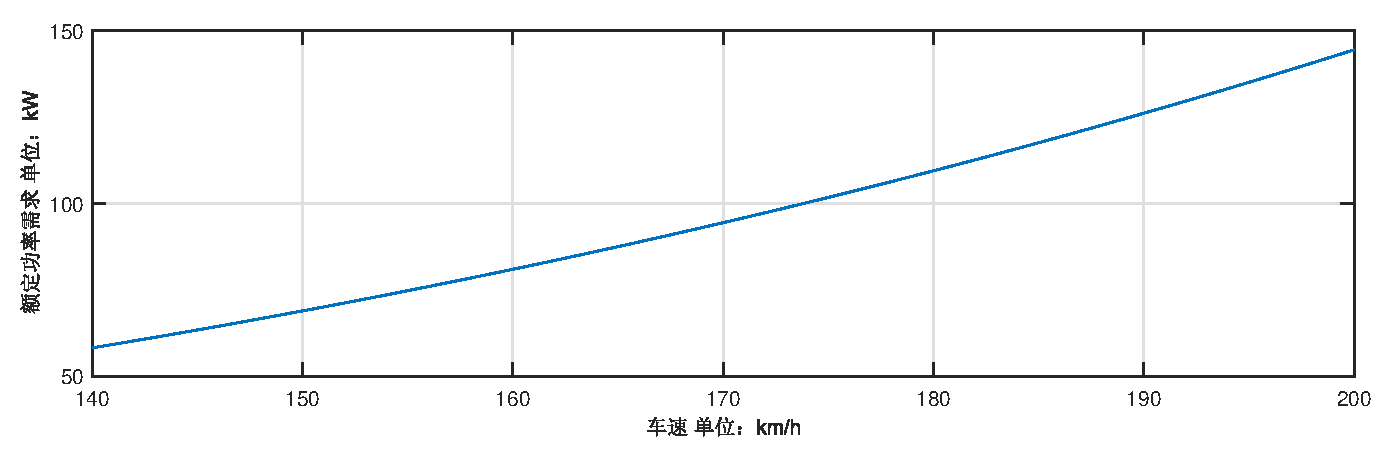
\includegraphics[width=0.9\textwidth]{figures/pe.eps}
	\caption{额定功率与最高车速图}\label{fig:pe}
\end{figure}

带入数据,计算得到的结果如图 \ref{fig:pe},电池额定功率取 $P_{e1}=68.89 kW$。

\subsubsection{爬坡度性能匹配}

当驾驶员驾驶车辆通过坡道路面的时候,车辆需要输出较大的扭矩,在爬坡状态下,车辆的行驶速度应该也能够得到保证,在表 \ref{tab:target} 中可以看到本文设计目标是车辆能够以 20km/h 的速度越过 30$^\circ$ 的坡道。同理,根据车辆平衡方程,爬坡度参数匹配的计算的公式如下所示:

\begin{equation}
	P_{e2} = v_{1} (G\sin\alpha_{max}+Gf\cos\alpha_{max}+\frac{C_DA}{21.15}v_{1}^2)/(\eta_T\eta_E)
\end{equation}

式中,$\eta_T$为机械效率,在这里取一般情况下的数据,$\eta_T = 96\%$,$\eta_E$ 为驱动电机的工作效率,在这里根据车型搭配的电动机万有特性曲线,取平均值 $\eta_E = 85\%$ 。$P_{e2}$ 为电池爬坡所需要的额定功率,$v_{1}$ 为爬坡时的车速,$f$ 为路面的滚动摩擦阻力系数,$\alpha$ 为本文预设的爬坡角度,在这里 $\alpha_{max}=\tan^{-1}(30\%)\approx 16.7^\circ$。
可以得到的额定功率应当满足条件:\ $P_{e2}= 40.53 kW$。

\subsubsection{加速性能匹配}
电动车辆起步的时候,车辆的扭矩需要满足一定值,否则车辆的加速性能较弱。电池箱的输出功率应该能够使得车辆的加速度满足表 \ref{tab:target} 中相关的要求。涉及到加速度的计算比较复杂,在这里本文假设车辆是按照恒功率 $P_{e3}$ 的状态进行起步加速的。

在匹配电池箱的加速性能参数时,应当把汽车的行驶方程改写,首先计算车辆的动力因数:

\begin{equation}
\begin{aligned}
	\label{equ:jiasu}
	D=\frac{F_t-F_w}{G}&=\frac{\frac{P_{e3}}{v\eta_T\eta_E}-\frac{C_DA}{21.15}v^2}{2020\times 9.8}\\
	\frac{\mathrm{d}v}{\mathrm{d}t}&=\frac{g}{\delta}(D-f)
\end{aligned}
\end{equation}

式中,$D$ 为匹配参数的车辆在加速时的动力因数,$f$ 为滚动阻力系数,$\delta$ 为该车辆的轿车旋转质量换算系数,计算匹配车辆的旋转质量换算系数的意义是,将车辆的因为车轮因为加速旋转而产生的阻力,经过计算等效成为车辆的平移驾驶时车辆的阻力。在一般的车辆的机械结构中,车辆的旋转质量换算系数主要受到车辆的飞轮和车轮以及传动轴影响,故在本文计算中,也仅仅将上述三个部件纳入转动惯量的计算过程中,在这里 $\delta$ 的计算公式如下 \cite{段建民2011串联式混合动力电动汽车复合电源系统设计}:

\begin{equation}
	\label{equ:rot}
	\delta=1+(0.02-0.04)+0.0015\times(i_{gi}i_0)^2
\end{equation}

上式中的 $i_{gi}$ 为当前档位的变速箱减速比,$i_0$ 为主减速器的主减速比。在这里 $i_{gi}i_0=6.1$。

根据式 \ref{equ:jiasu} 计算并绘制出车辆的加速度$a$与车速$v$关系图,如图 \ref{fig:a-v}。根据路面的摩擦系数限制条件 \cite{胡朋2011不同状态下路面摩擦系数现场试验},车辆的加速度阈值大小被设定在 0.63G。

\begin{figure}
	\centering
	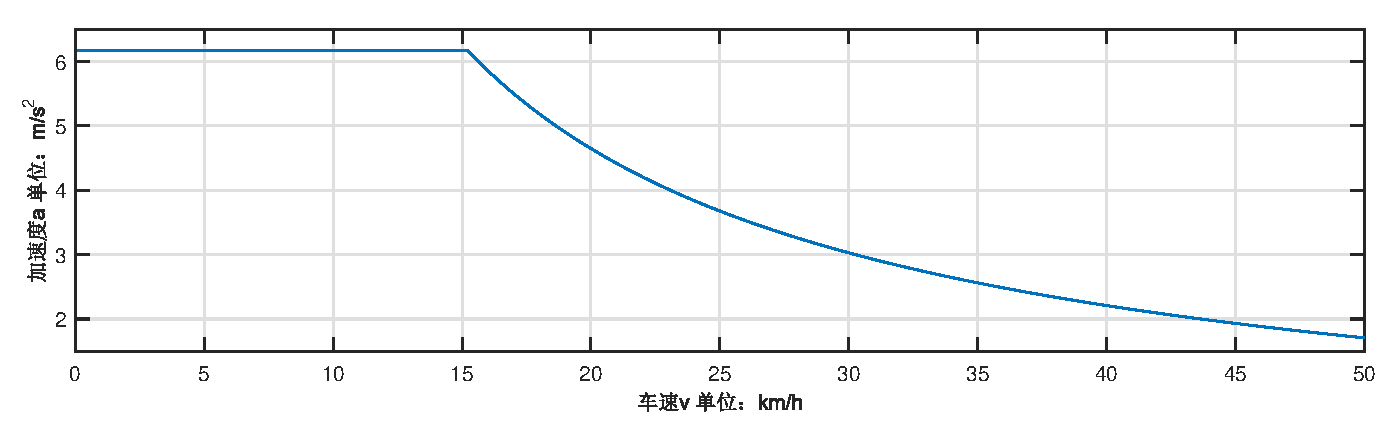
\includegraphics[width=0.9\textwidth]{figures/a-v.eps}
	\caption{车辆的加速度$a$与车速$v$关系}\label{fig:a-v}
\end{figure}

将其转化为车辆的加速度的倒数$\frac{1}{a}$与车速$v$关系图,如图 \ref{fig:aa-v}。

\begin{figure}
	\centering
	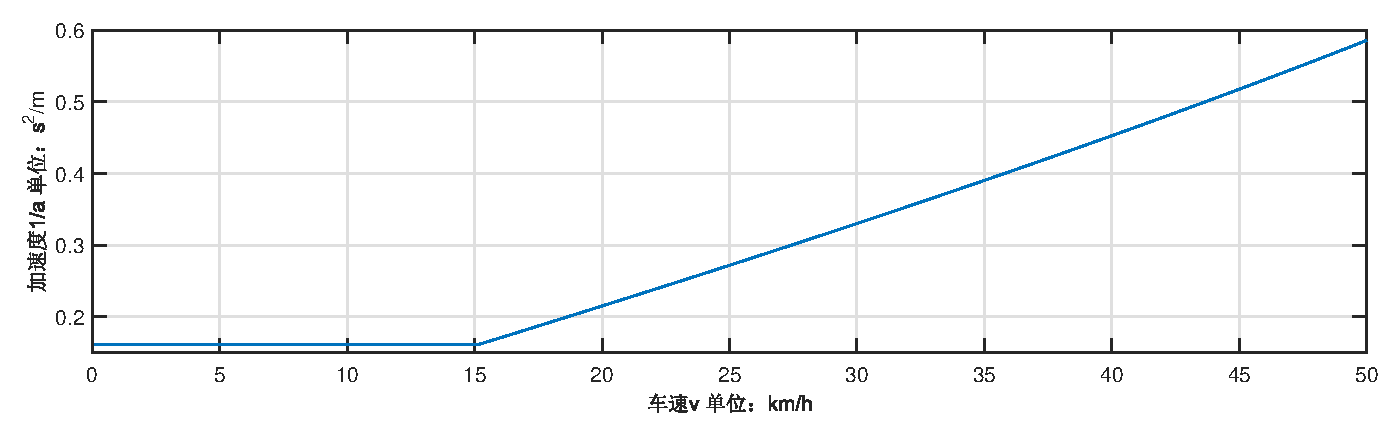
\includegraphics[width=0.9\textwidth]{figures/aa-v.eps}
	\caption{车辆的加速度的倒数$\frac{1}{a}$与车速$v$关系}\label{fig:aa-v}
\end{figure}

计算其对于 x 轴积分即可得到加速度时间值,根据计算,当车辆满足 0$\sim$50km/h 加速时间小于 15 秒时,电池箱的输出功率为 $P_{e3}=68.5 kWh$。

根据以上的计算结果 $P_e=max(P_{e1},P_{e2},P_{e3})=P_{e1}=68.89 kW$,可以满足最高车速超过 150 km/h 的行驶需求。每块电池的额定放电倍率为 6C,则每块电池的额定功率为 $P_0=U_0I_0=3.65 \times 6 \times 37 =810.3 W$,最少需要的电池单体块数为:

\begin{equation}
	n_1=\frac{68.89\times 1000}{810.3}\approx 86
\end{equation}

\subsection{电池包容量计算}
电池包的容量是反映电池系统能够储存多少电能的参数,是电池系统最重要的参数之一,在设计时,电池包的容量参数决定了电池系统有多少块电池单体组成。
电池包的容量要求主要来自于车辆的行驶里程需求,根据目前市面上常见的混合动力汽车的参数列表,如表 \ref{tab:car_group} 和图 \ref{fig:car_group}。可以看到,大部分车型的纯电动里程在 40-59 km 之间,为了保证汽车的纯电动里程符合使用要求,本文将预期的电动车续航里程确定为 60 km。

\begin{table}
	\centering
	\caption{不同品牌的混合动力汽车参数}\label{tab:car_group}
	\begin{tabular*}{0.9\textwidth}{@{\extracolsep{\fill}}ccc}
		\toprule
		厂家			&车型                   &纯电动里程		 \\
		\midrule
		通用	        &Chevy Volt             &85        \\
		宝马		    &i8                     &23 \\
		奥迪            &A1 E-tron              &50         \\
		奥迪            &A3 Sportback E-tron    &27            \\
		保时捷          &Panamera S E-hybrid    &26            \\
		福特            &C-MAX Energi           &31           \\
		福特            &Fusion Energi          &34         \\
		现代            &Sonata PHEV            &43         \\
		现代            &Ioniq PHEV             &47          \\
		凯迪拉克        &ELR                    &58          \\
		凯迪拉克        &CT6 PHEV               &50          \\
		丰田            &Prius Prime            &40      \\
		本田            &Clarity PHEV           &76      \\
		克莱斯勒        &Pacifica Hybrid        &53       \\
		沃尔沃          &XC90 AWD T8 PHEV       &27       \\
		起亚            &Niro PHEV              &42      \\
		起亚            &Optima PHEV            &47      \\
		\bottomrule
	\end{tabular*}
\end{table}

\begin{figure}
	\centering
	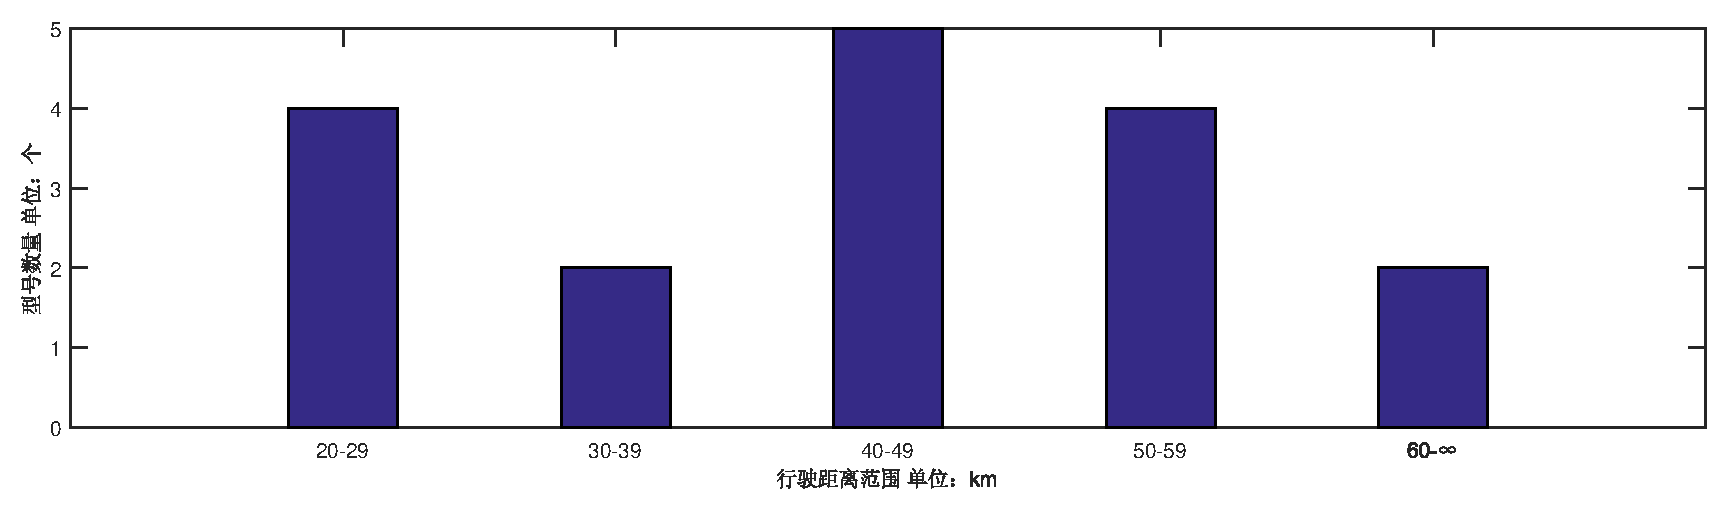
\includegraphics[width=0.9\textwidth]{figures/car_group.eps}
	\caption{不同续航里程区间车型数量}\label{fig:car_group}
\end{figure}

电动车的能量消耗计算时所使用的测试环境是根据中国的典型道路工况决定 \cite{刘希玲2000我国城市汽车行驶工况调查研究},根据《电动汽车能量消耗率和续驶里程试验方法(GB/T 18386-2017)》 标准中规定的 NEDC 工况进行相关的理论计算 \cite{叶磊2012基于中国典型城市循环工况的动力电池测试评价方法},NEDC 工况的速度与时间的关系图如图 \ref{fig:NEDCv},加速度与时间的关系如图 \ref{fig:NEDCa} \cite{kim2009model}。根据 NEDC 工况的速度与加速度数据,和上述车辆的功率平衡方程 \ref{equ:powerequ} ,化简得到式 \ref{equ:powerequ2}。

\begin{figure}
	\centering
	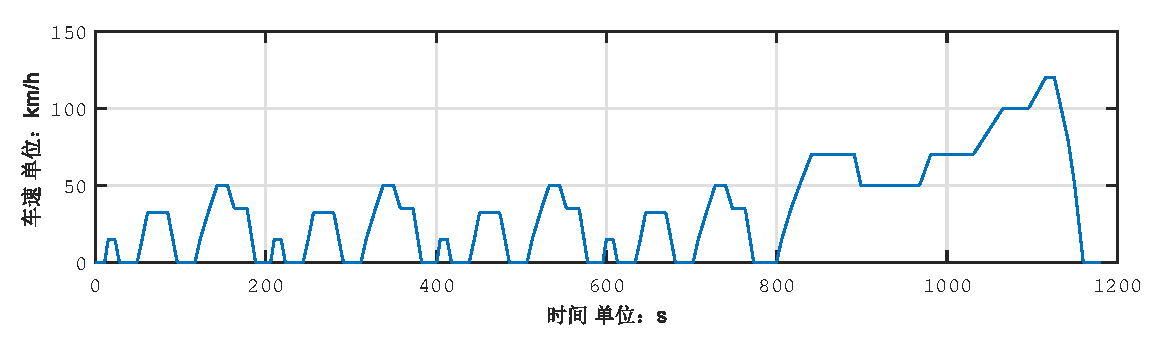
\includegraphics[width=0.9\textwidth]{figures/NEDCv.eps}
	\caption{NEDC 工况速度-时间分布图}\label{fig:NEDCv}
\end{figure}

\begin{figure}
	\centering
	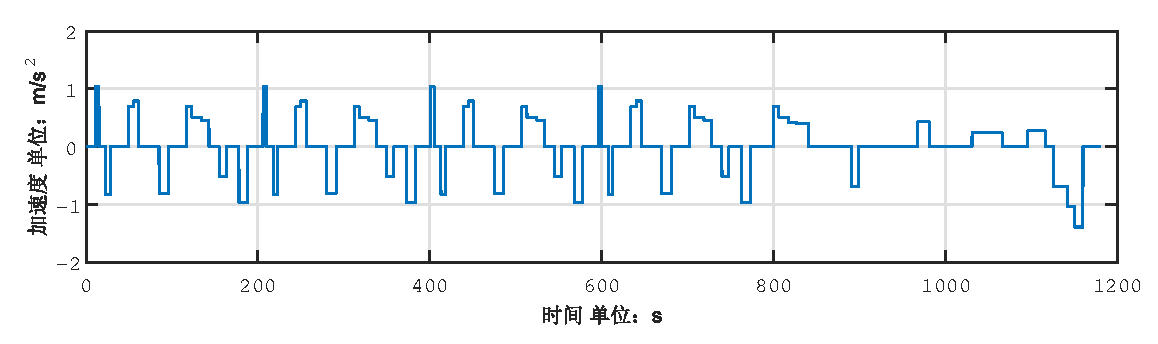
\includegraphics[width=0.9\textwidth]{figures/NEDCa.eps}
	\caption{NEDC 工况加速度-时间分布图}\label{fig:NEDCa}
\end{figure}

\begin{equation}
	\label{equ:powerequ2}
	\eta_T\eta_EP_e=\frac{Gfv_a}{3600}+\frac{C_DAv_a^3}{76140}+\frac{\delta mv_a}{3600}\frac{\mathrm{d}v}{\mathrm{d}t}
\end{equation}

式中的 $P_e$ 为平衡状态的发动机输入功率,$G$ 为匹配所选车辆的自身重量(满载),$f$ 为车辆的滚动摩擦力,$v_a$ 为车辆的运行车速,$C_D$ 为空气阻力系数,$A$ 为迎风面积,$\delta$ 为轿车旋转质量换算系数。

通过计算得出中国典型道路工况功率图(含制动再生)和能量的消耗图 \cite{高建平2015插电式混合动力汽车车载复合电源功率分配策略研究},分别如图 \ref{fig:NEDCp},图 \ref{fig:NEDCe}。
\begin{figure}
 \centering
 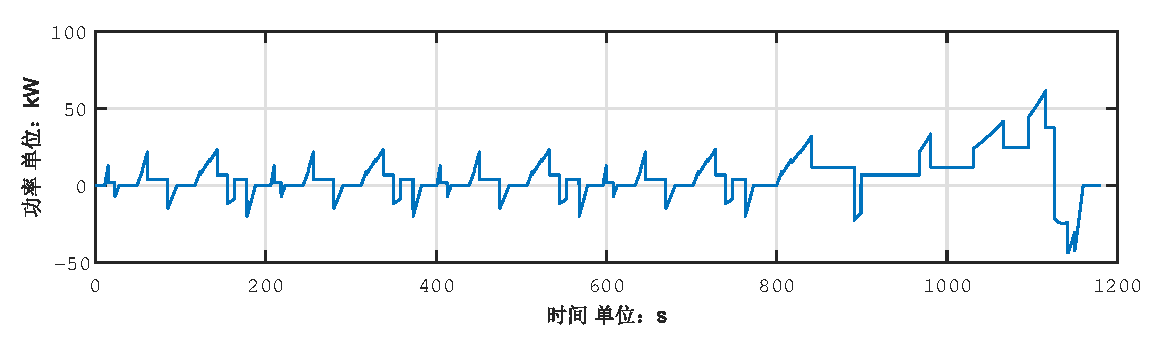
\includegraphics[width=0.9\textwidth]{figures/NEDCp.eps}
 \caption{NEDC 工况功率-时间分布图}\label{fig:NEDCp}
\end{figure}

\begin{figure}
 \centering
 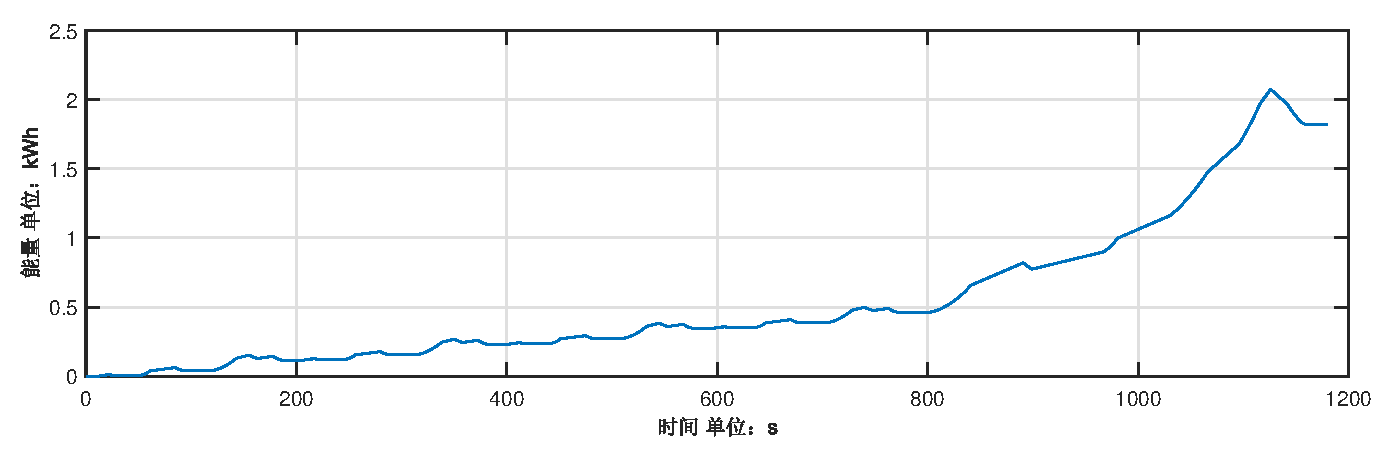
\includegraphics[width=0.9\textwidth]{figures/NEDCe.eps}
 \caption{NEDC 工况能量消耗-时间分布图}\label{fig:NEDCe}
\end{figure}

NEDC 循环工况的总路程为 11.022 km,根据上述计算结果,完成一次 NDEC 循环,该车型需要消耗 1.823 kWh 能量,等效百公里的平均能量消耗为 16.540 kWh。60 公里的里程理论需要 9.924 kWh 的蓄电池能量,等同于电池单体块数:

\begin{equation}
	n_2=\frac{9.924\times 1000}{3.65 \times 37}=73 < 86
\end{equation}

根据能量计算和功率计算得到的电池单体块数限制,可以得到,最终的电池组中的电池单体的数量不应少于 86 块。而电动汽车的电压平台受到了电机控制器和电机额定电压的限制,一般的电动汽车的高压平台电压在 300 至 500 伏之间,在本文的设计中,为了便于电池包的模组设计,故选择 88 个电池单体构成电池系统,并将其分成 8 个模组,每个模组含有 11 个电池单体,电池箱的总额定电压为 321.2 伏。

根据本文最终的设计,可以计算得到电池箱的理论参数,如表 \ref{tab:box}。

\begin{table}
	\centering
	\caption{设计的电池箱理论参数} \label{tab:box}
	\begin{tabular*}{0.9\textwidth}{@{\extracolsep{\fill}}cc}
		\toprule
		参数项目			&数值		 \\
		\midrule
		电池块数/块	     &88  \\
		额定能量/kWh     &11.884  \\
		额定功率/kW      &71.306  \\
		额定内阻/$\Omega$ &1.584  \\
		续航里程/km      &71.852  \\
        最高车速/(km/h)  &152   \\
		\bottomrule
	\end{tabular*}
\end{table}

\section{整车仿真}

上述的理论计算过程得到了电池箱相关的理论参数,为了验证参数的有效性和准确性,本文使用了 AVL Cruise(下称 Cruise)软件,该软件内置一些数据求解器,可以根据输入的整车参数和车辆传动模型,在各种模拟的工况条件下进行测试,并取得模拟车辆的测试结果。Cruise 软件中,模拟车辆的模型采用可视化模块界面,使用者可以很方便的通过使用软件提供的车辆各个组件,修改它们的参数,或者相互组合。并且 Cruise 软件内部内置了丰富的工况模型,例如 NEDC 和 FTP 75 工况,大大简化了在普通车辆计算中的繁琐的工况信息输入过程。

\subsection{整车信息输入}

在使用 Cruise 软件搭建相关的车辆参数模型时,要首先输入车型的整车信息,包括车辆的重量,迎风面积,轴距和轮距等信息,在这里,本文仿真过程中,在 Cruise 软件内输入的相关整车信息如表 \ref{tab:carinfo} 所示。

\begin{table}
	\centering
	\caption{在 Cruise 软件内设置的整车参数} \label{tab:carinfo}
	\begin{tabular*}{0.9\textwidth}{@{\extracolsep{\fill}}cc}
		\toprule
		参数项目			&数值		 \\
		\midrule
		Curb Weight(整备质量)/kg	     &1540  \\
		Gross Weight(满载质量)/kg     &2020  \\
		Frontal Area(迎风面积)/$m^2$      &2.6667\\
		Drag Coefficient(空气阻力系数)     &0.35  \\
		\bottomrule
	\end{tabular*}
\end{table}

在输入完成整车信息之后,还应该设置车辆的驾驶阻力模型,在仿真过程中,车辆阻力是一个至关重要的参数,特别是进行有关车辆的能量消耗和油耗等方面的仿真方面,该参数的模型准确性对于仿真结果影响巨大。该参数在之前的电池包理论计算中被分为四项,分别为滚动阻力,加速阻力,坡道阻力和空气阻力,具体信息参见式 \ref{equ:powerequ}。在 Cruise 软件中,阻力模型被分为若干种阻力模型,车辆物理模型,一阶线性模型(速度),二阶线性模型(速度和速度平方),本文在理论计算的过程中使用的模型为物理模型,该模型下车辆的阻力模型与车辆的空气阻力和车辆轮胎的滚动阻力有关。

\subsection{组建车辆动力模型}

当完成了车辆的整车信息输入之后,接下来是要完成对于车辆的动力模型的构建,本文选用的模型为串联式混合动力模型,搭建的模型的结构如图 \ref{fig:car_structure} 所示。其中,设置的主减速比为 6.058(根据电机的最高转速和车辆的轮胎滚动半径计算得到),主减速器的机械效率为 $96\%$,差速器的效率设定为理想值 $100\%$,总传动链的机械效率为 $96\%$,与理论计算时的机械效率保持一致。

\begin{figure}
	\centering
	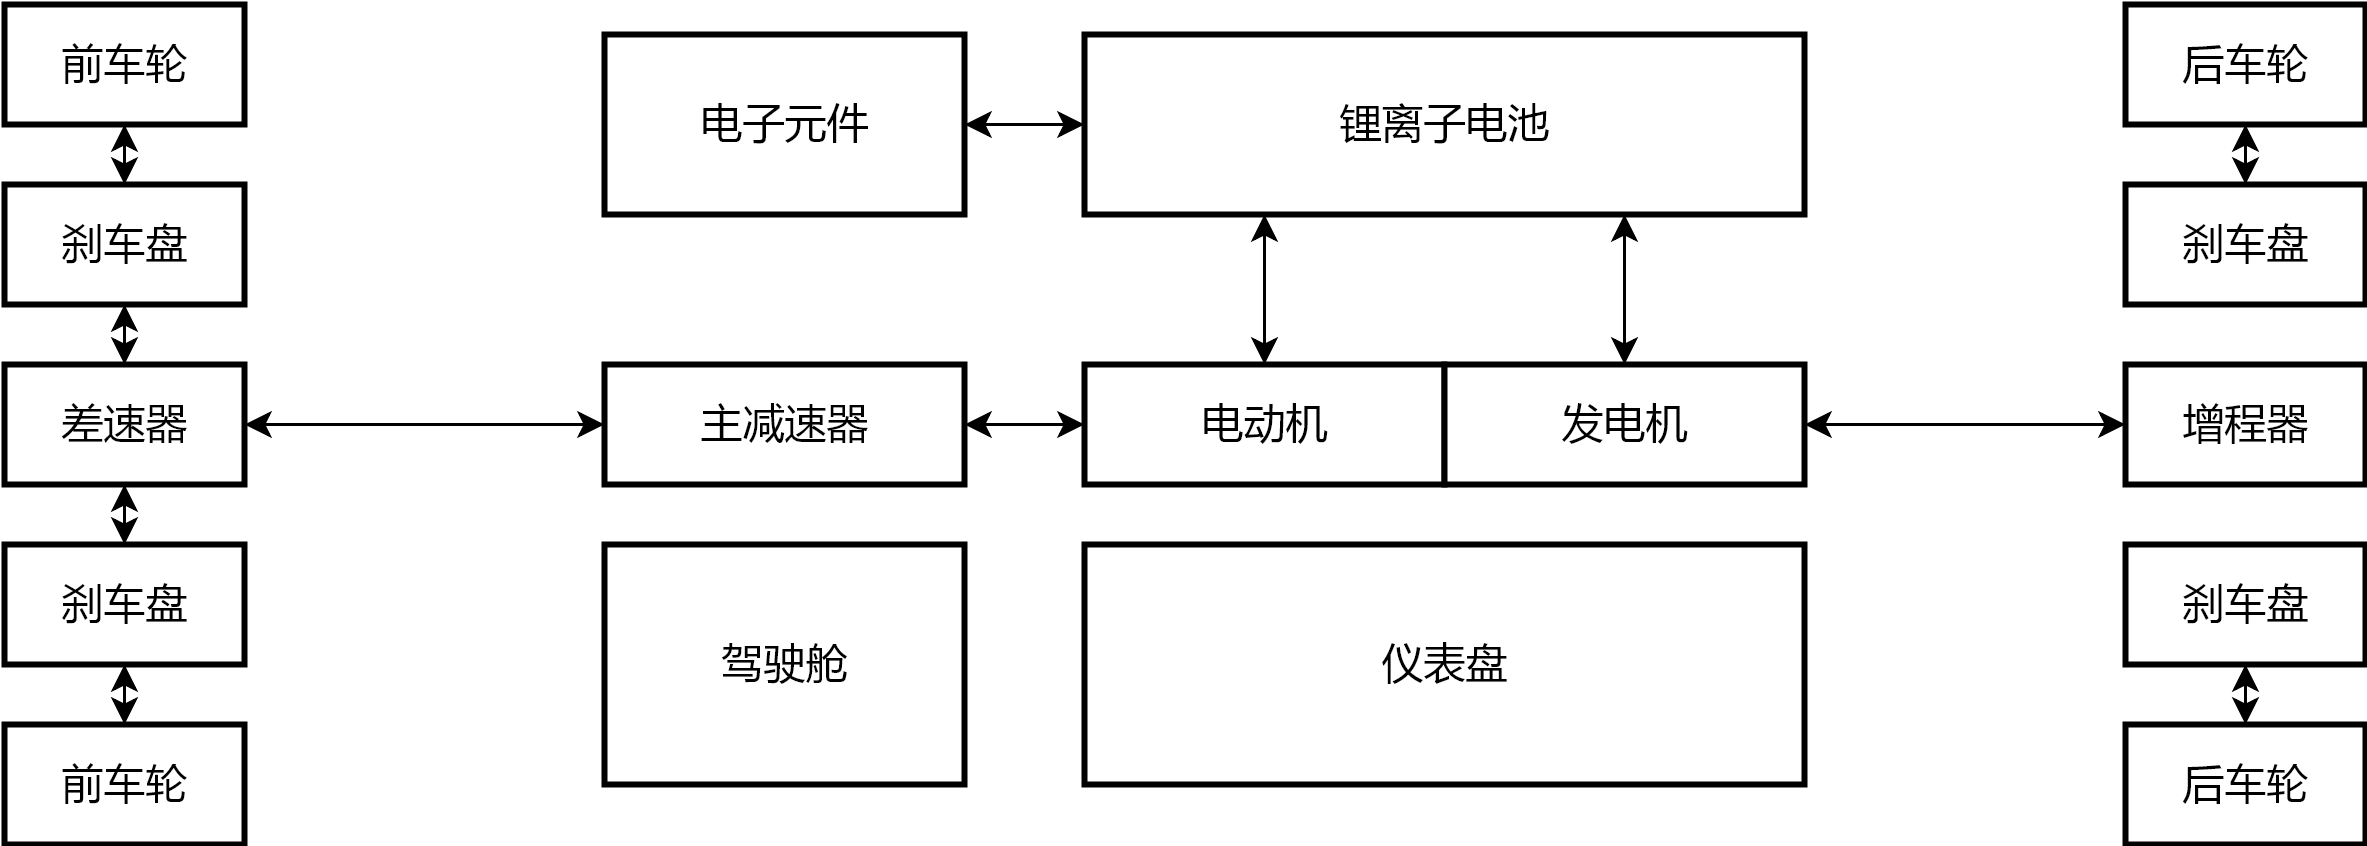
\includegraphics[width=0.75\textwidth]{figures/car_structure_cruise.png}
	\caption{Cruise 车辆动力模型}\label{fig:car_structure}
\end{figure}

在车辆运行时轮胎的滚动阻力系数与车速有关,由于轮胎与地面间存在振动,随着车辆的行驶车速上升,轮胎的响应振动频率随之上升,当到达某一定值时轮胎的表面会发生驻波现象,轮胎的外边缘会变成波浪状,造成阻力系数剧烈提升。而轮胎的滚动阻力系数与多种因素有关,包括轮胎的充气压力,轮胎的帘线类型,轮胎的橡胶种类有关。该仿真车辆轮胎的滚动阻力系数特性曲线参见图 \ref{fig:tier_characteristics}。

\begin{figure}
	\centering
	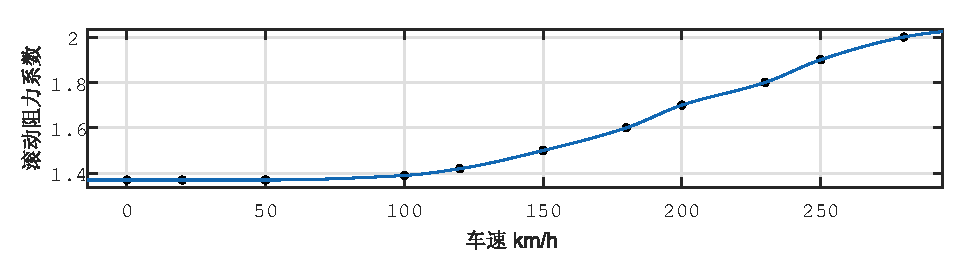
\includegraphics[width=0.9\textwidth]{figures/tier_characteristics_cruise.eps}
	\caption{仿真中的轮胎滚动阻力特性曲线}\label{fig:tier_characteristics}
\end{figure}

\subsection{电动机参数设定}
在本次仿真过程中,使用的电动机模型为软件自带的电动机模型,电机类型为异步电动机,额定电压设定为 320V,最高转速为 10000 rpm,该电机的万有特性曲线如图 \ref{fig:asm_characteristics} 所示。

\begin{figure}
	\centering
	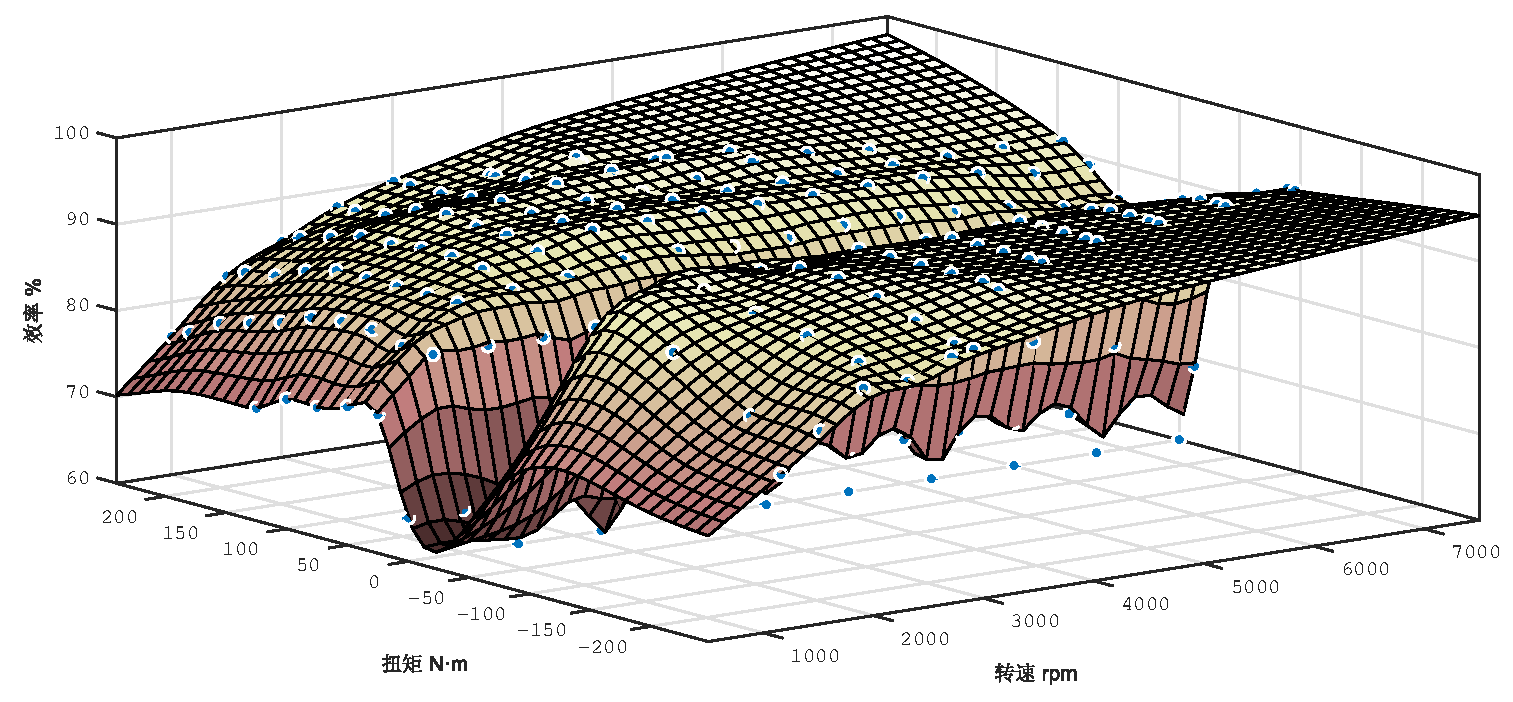
\includegraphics[width=0.9\textwidth]{figures/asm_characteristics_cruise.eps}
	\caption{电机的万有特性曲线}\label{fig:asm_characteristics}
\end{figure}

在之前的理论计算中,本文使用的电机效率为该电机万有特性曲线获得的平均值 $85\%$。

\subsection{电池箱参数设定}
接下来进行的是电池箱参数的设定,电池箱设定的参数根据厂家提供的电池单体信息和本文设计的参数,其中电池单体参数参见表 \ref{tab:cell} 所示数据。而电池的 OCV-SOC 曲线为实验室测的的数据,如表 \ref{fig:cell-OCV} 所示。

\begin{figure}
	\centering
	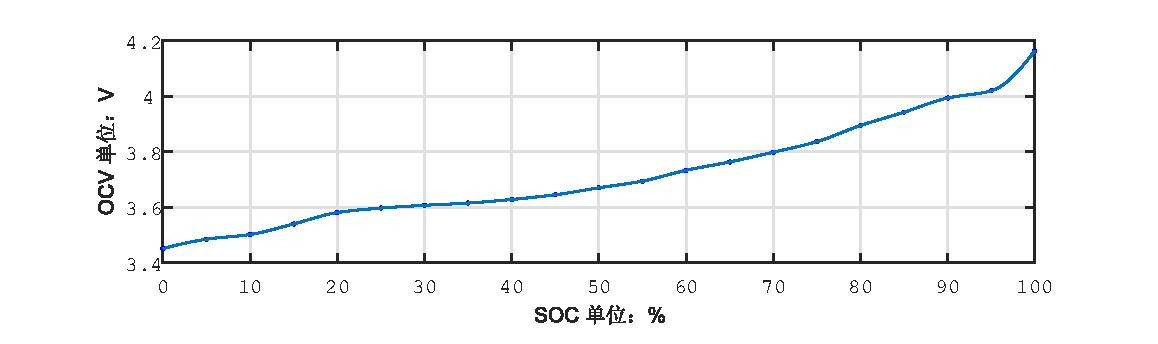
\includegraphics[width=0.9\textwidth]{figures/cell-OCV.eps}
	\caption{LP2714897 电池单体 OCV-SOC 特性曲线(实验获得)}\label{fig:cell-OCV}
\end{figure}

根据上述匹配的结果,输入对应的电池连接方式,为 88 个电池单体串联的方式进行连接。

\subsection{仿真工况与驾驶员设定}
Cruise 软件自带了许多工况信息,本文使用了其中预置的 NEDC 工况,该工况的信息见图 \ref{fig:NEDCv}。在仿真过程中使用的模型是车辆的物理运动模型,车辆为满载状态下的情况。驾驶员驾驶习惯状态如表 \ref{tab:driver} 所示。当仿真开始时,电池箱的 SOC 值被设定为 $100\%$。

\begin{table}
	\centering
	\caption{Cruise 驾驶员习惯} \label{tab:driver}
	\begin{tabular*}{0.9\textwidth}{@{\extracolsep{\fill}}cc}
		\toprule
		参数项目			&数值		 \\
		\midrule
		Starting Speed(开环起步转速)/rpm	     &4000     \\
		Customer Starting Speed(闭环起步转速)/rpm &1200  \\
		Maximum Brake Force(最大刹车踏板力)/N      &10   \\
		Foresight Time(前瞻时间)/s      & 0.25      \\
		\bottomrule
	\end{tabular*}
\end{table}

\subsection{Cruise 仿真结果}
软件仿真后的结果被分为数类,其中包括了车辆的运动参数,车辆的电池箱参数,车辆的驾驶员姿态参数,道路参数。其中,本文只对于电池箱的有关参数进行分析,在行驶的整个过程中,电池箱有关参数的变化如图 \ref{fig:result} 所示。

\begin{figure}
	\centering
    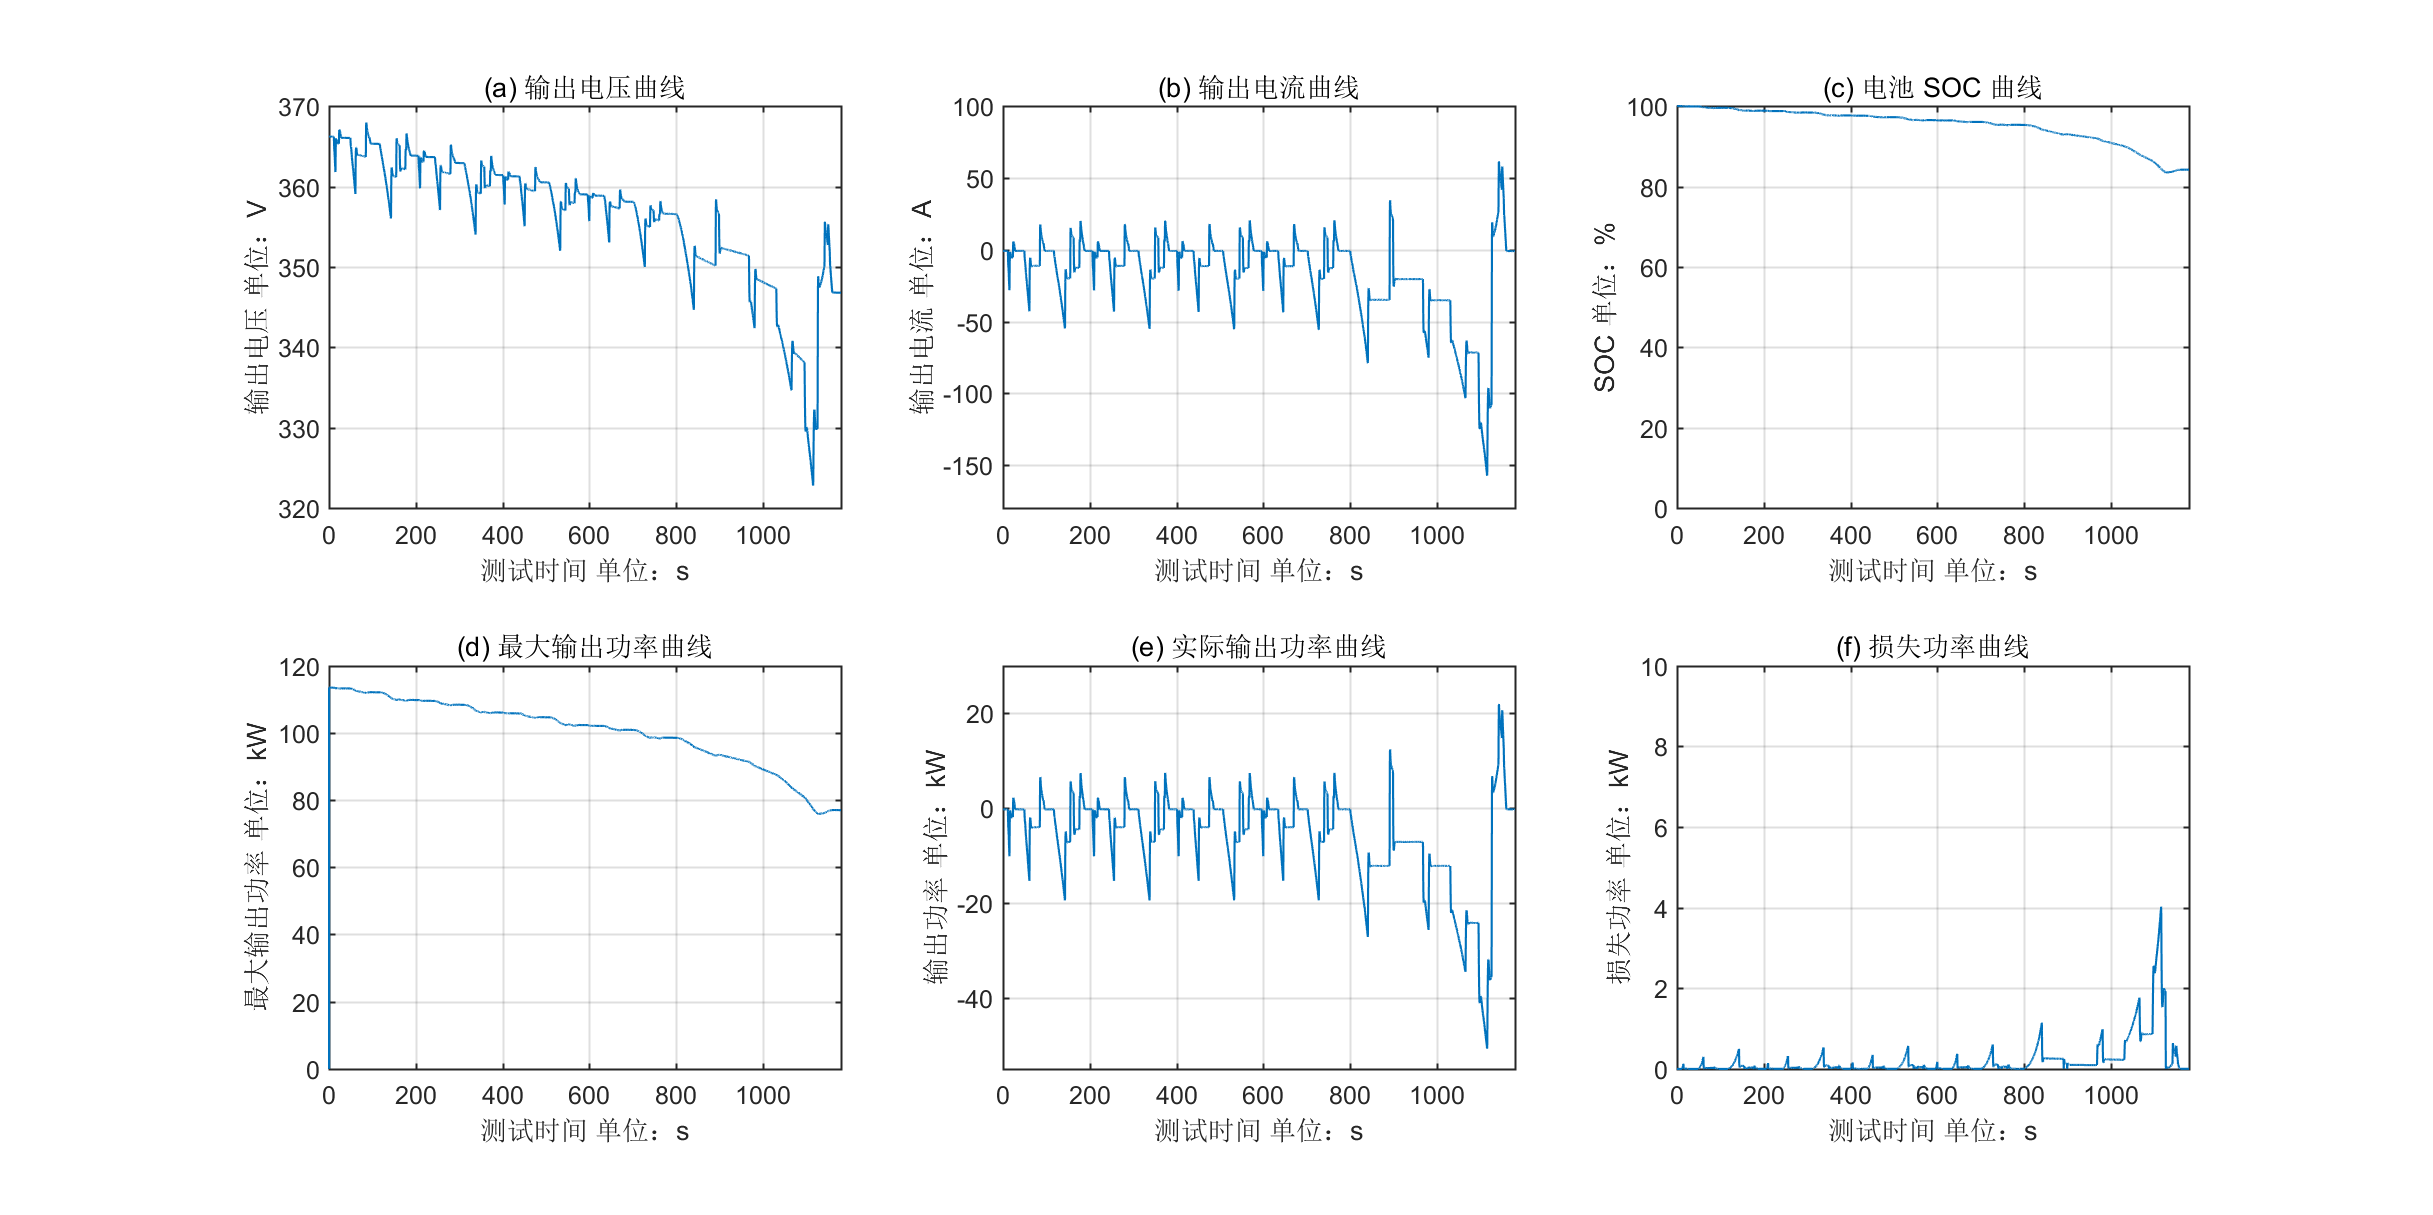
\includegraphics[width=1\textwidth]{figures/result.eps}
	\caption{Cruise 仿真结果}\label{fig:result}
\end{figure}

可以看出,仿真的过程中,电池箱未发生功率不足的情况,电池箱的最大输出功率始终超过电池箱的输出功率,这证明了电池箱在输出功率方面符合了要求,电池箱的功率计算有效。在完成了一次 NEDC 的循环后,电池箱的剩余电量为 31.1477 Ah,消耗的电量为 5.8523 Ah。根据仿真结果,计算总计的续航里程为 $S_D=\frac{37 \times 11.022}{5.8523} = 70.035 km$,与通过理论计算得到的(参见表 \ref{tab:box})数据基本一致,仿真结果与理论计算的相对误差为 $2.6\%$,可以认为理论计算的结果具有有效性,并且比较准确。

\section{理论计算误差分析}
关于上述理论计算的过程中存在的误差,下文将误差因素进行了一个总结,并且对于弥补误差,获得更精确的理论计算值提供了一个方法,希望能供后续的研究参考,并且改进计算模型。实验误差的种类分为系统误差和随机误差,但是由于该计算过程仅仅使用计算机模拟仿真,各个参数对于结果的影响均包含在系统计算范围之内,可以人为进行控制,故可以认为仿真的测量值不存在随机误差。所以下文的误差分析仅仅针对于系统存在的误差进行分析。

\subsection{电池参数误差}

\subsubsection{电压误差}
厂家提供的电池单体参数,参见表 \ref{tab:cell},对于电池的额定电压,在参与理论计算的计算过程中被当做一个固定不变的值,本文对于电池容量的计算也仅仅通过对于额定电压和安时数进行简单的相乘计算,而在实际情况下,电池的输出电压是一个和电池电量相关的数值,在实验室数据中,随着电池的放电,电池的电量下降,电池的开路电压(OCV)也随之发生了改变,如图 \ref{fig:cell_deviat} 所示,实验室数据和理论计算时使用的数值有偏差。因为上述理论计算过程中采用的容量计算方式是根据电池安时和电池的额定电压数据进行计算的,故当电池的开路电压发生了改变,电池的容量估计便存在误差,对于计算结果产生了影响。

\begin{figure}
	\centering
	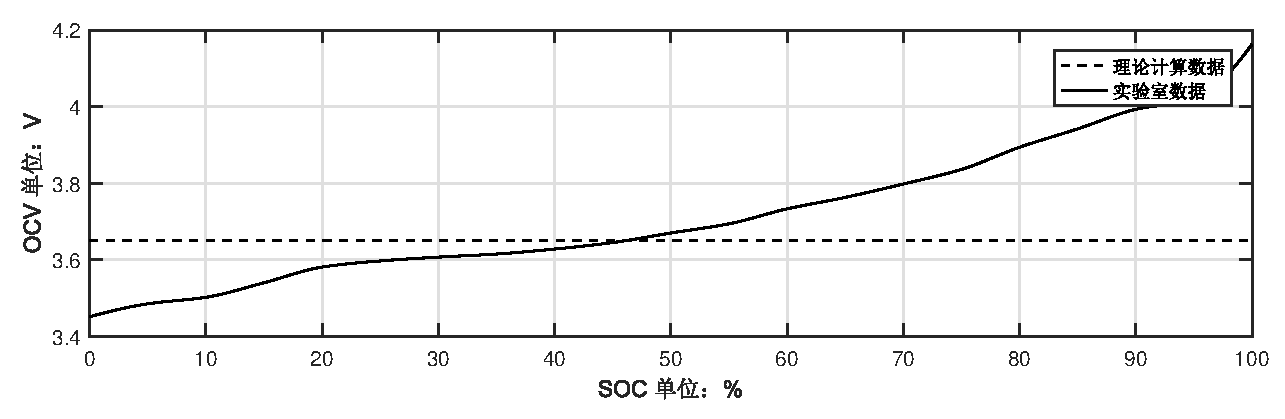
\includegraphics[width=0.9\textwidth]{figures/cell_deviat.eps}
	\caption{电池单体的 OCV 计算偏差}\label{fig:cell_deviat}
\end{figure}

这也就是说在理论计算的过程中,电池的电压模型建模不够精确,如果想要更加精确的计算结果,可以在系统中输入电池的 OCV-SOC 曲线,根据电池的 OCV 曲线,结合安时计测量,获得电池的准确电量值。该值不仅仅对于电池的的容量有影响,可以看出,在仿真曲线的后期,由于 SOC 的下降,电池的开路电压下降,导致电池包的输出电压大幅度下降,而由于车辆的阻力和车速未发生变化,维持车辆所需要的输出功率并没有发生改变,导致电池包的输出电流剧烈上升。在这种情况下,电池包的总输出电流会超过理论计算中的值,造成线路承受巨大的电流,有安全风险。

\subsubsection{内阻误差}
在本文的理论计算章节,忽略了电池内阻的影响,而在理论仿真的过程中,对于内阻的设置,也仅仅设置了一个固定的内阻值,而在实际的使用当中,内阻对于电池放电的影响十分重大,不可忽视。首先,在电池的能量计算中,电池输出的能量多少与内阻的高低相关,由于电池采用安时计算的方式计算能量,在电池放电或充电的过程中,电池内阻会消耗电能,并产生焦耳热 $I^2R \delta t$,可以看到,焦耳热的多少与电流的平方成正比,故在大倍率、高电流的放电情况下,电池的内阻产生的焦耳热会大大增加。根据研究结果,电池的内阻是一个与电池的 SOC 以及温度息息相关的的值,当电池的 SOC 下降的情况下,电池的内阻值会逐渐上升,而在温度较低的环境下电池的内阻也会显著上升,电池内阻会影响电池的容量 \cite{刘伟2016锂离子动力电池直流内阻测试及其应用研究}。其次,电池的输出功率与电池的内阻有关,当电池的内阻为 $\gamma$ 时,电池理论上无法输出超过 $\frac{U_ocv}{\gamma}$ 的功率。相比纯电动汽车,混合动力汽车中搭载的电池单体数量较少,在相同的功率需求条件下,电池的充放电倍率较大,电池内阻过大会导致电池输出功率不足,在车辆需要大功率输出的时候,电池不仅无法提供足够的输出功率,还会产生电池过放的风险,使电池处于不安全状态。

在理论计算中,可以先在实验室内控制环境条件,譬如气温的高低。在不同的 SOC 以及温度条件下测量电池的内阻值,并建立电池的内阻模型,根据电池的 SOC 情况使用不同的内阻值,一般情况下,电池的 SOC 值越低,电池的内阻就会相应的有所提高,电池箱的放电倍率越大,电池的内阻上升越快 \cite{罗玉涛2016延长锂离子电池寿命的电动汽车复合电源设计};并计算电池的内阻产生的热量,对于电池的温度模型进行建模仿真,仿真出电池包在运行的时刻的不同温度条件下的内阻情况,将两种因素(温度以及 SOC)同时带入能量计算的过程,可以获得更加精准的电池能量输出量,这会对于车辆的行驶里程等容量相关的计算结果更加精确可靠,并且可以验证电池包的输出功率是否能够满足使用要求。

\subsection{电机参数误差}

本文理论计算中有关电机的参数仅有电机的效率参与了计算,而在实际的仿真中,是使用了电机的万有特性曲线进行效率的计算,这之间的不同就涉及到了电机效率参数的误差。

电动机类似于内燃机,在实际的工作情况下,其工作效率同样受到其转速和负载转矩的影响,但普通的特性曲线仅仅只能表示两种参数之间的关系,而不能表示三种参数的相关关系,于是电动机也存在万有特性曲线。电动机的万有特性曲线的横坐标为电动机的转速和负载转矩,纵坐标为电动机的能量转换效率。在理论计算过程中,本文使用了平均的电机的能量转换效率,即为 $85\%$。但是在实际的情况下,电机的能量转换效率在不同的车速情况下,也会发生变化,如图 \ref{fig:asm_characteristics} 所示。此误差会导致理论计算的时候,电池箱的功率与实际的输出值不符合,存在一定的误差。

可以在计算的时候,在每一时刻的情况下,根据车速和车辆的加速度状态,与车辆的主减速器,计算出车辆的每一时刻的电机的负载转矩和转速。根据这两个因素计算电动机的能量转换效率,并参与电动机的输出功率的计算,使用这种方法得到的输出功率曲线才是更加精确的理论值。

\subsection{车辆动力模型参数误差}
在计算的过程中,本文使用的车辆动力模型是依照纯物理模型建立的模型,是根据汽车的车速,加速度计算的。但是在实际情况下,汽车的阻力模型是一个与许多因素有关的复杂的模型,不仅仅与外部环境譬如温度,路面不平度,路面的摩擦系数,空气密度,风阻有关,也与车辆的结构有关,譬如车辆的空气动力学模型,车辆的轮胎刚度,车辆的悬架刚度等等因素有关。当然在计算的过程中,考虑到所有的因素是不可能的,但是可以通过一系列的矫正系数,来使本文的计算结果更加逼近实际测量值,但是这需要大量的实验数据作为基础。

在计算的过程中,本文忽视了各种动力系数的变化,在车辆进行低速到高速的变速运行的情况下,车辆的空气阻力系数,轮胎滚动阻力系数也会发生改变,可以测量车辆的各项参数在不同车速条件下的值,并对于计算结果进行校正;在车辆的传动链上,差速器和减速器也会根据车速的不同,产生机械转换效率的改变,如果想要更加精准的测量值,可以根据各个部件的这种改变也可以在后续的改良计算中进行改良,来获取更加精确的效率系数。

在本文的理论计算中,对于旋转质量系数的计算公式是采用经验计算公式确定的,如式 \ref{equ:rot},但是该计算公式在车辆的质量,车辆的传动结构发生差异也会产生差异,如果想要更加精确地结果可以根据指定车辆的结构计算此系数,会使结果更加精确。

在设计电池系统参数的时候,设计完成的参数应用于电池箱之后,一旦电池系统参数发生改变,同样会改变电池箱的物理参数,例如根据电池箱的参数大小决定电池箱内部使用多少块电池单体,这会导致电池箱的大小和质量等等参数发生。因为电池箱是安装在车辆上的部件,电池箱的质量会影响车辆的物理特性,包括车辆的轴荷状态和车辆的阻力等相关系数。也就是说在设计完成后,电池箱的参数会反而影响所匹配的车辆的运行状态。在理论计算中,本文将车辆的质量固定为满载状态,不受电池箱的质量影响,而在实际的应用当中,电池箱由于质量较大,其参数对于车辆的影响同样较大,故如果想要获得更加精确的车辆阻力模型需要在理论计算环节考虑到电池箱参数对于车辆整体的动力学模型的影响。


%%==================================================
%% chapter02.tex for BIT Master Thesis
%% modified by liu xiahua
%% version: 0.1
%% last update: May 20th, 2018
%%==================================================

\chapter{电池箱机械设计}
\label{chap:engineering}

在本章,本文将会就上一章所设计的电池箱系统参数,对于该电池箱进行机械结构的设计和校核,混合动力汽车的电池箱结构设计与纯电动汽车的电池箱结构基本类似,但是由于其电池的数量较少,所以混合动力电池箱的结构较为简单,但是设计的时候应该遵守电池箱设计标准。因为车载电池的工作环境较差,电池箱需要承受来自车身的振动 ,加速度,以及电池箱内部产生的热量,在国外,有研究认为,环境温度,压力,机械振动等电池包所在的长期环境条件,会对电池可靠性产生重大影响 \cite{王文伟2016电动汽车电池箱结构随机振动疲劳分析}。也有研究认为,温度也影响锂离子电池包的可靠性和电池的循环寿命 \cite{能量效率和工作温度对锂离子电池剩余寿命的影响}。所以电池箱的结构设计在电动汽车领域占有一定的比重。

\section{现有标准相关信息}

由于目前电动车市场已经逐渐成熟,电池箱结构与安全方面的相关的标准制定已经相当完善,在美国 SAE 协会制定了许多相关的电动车标准,如表 \ref{tab:SAE_standard} 所示,电池箱相关的结构设计标准在电池极耳和母线的连接方式,电池的布置方面进行了详细的叙述,对于电池的热失控的控制等安全性问题也进行了相关的解决方案的规定,对于电池系统的热管理系统进行了方案的提出。

传统的电池箱设计是针对于电池箱模组的安全设计和检查的,本文对于电池箱的模组设计充分考虑到了安全因素,并且在模组范围之外,本文还对于电池箱整体与车体的连接进行了设计校核 \cite{Dubarry2009From}。在电池与车辆的连接部分处承受着来自电池箱的巨大重量,并且由于第一章匹配对应的电池箱的质量较重,故其惯性较大,在车辆产生振动或者加速减速的状态下,电池箱安装框架连接部分会产生较大的应力,故校核框架的连接强度是十分必要的。

\begin{table}
	\centering
	\caption{SAE 对于电池箱机械结构和安全方面的标准} \label{tab:SAE_standard}
	\begin{tabular*}{0.9\textwidth}{@{\extracolsep{\fill}}cp{5cm}p{5cm}}
		\toprule
		\textbf{标准} & \textbf{题目} & \textbf{简介} \\
		\midrule
		SAE J240 & Life test for Automotive Storage batteries & 车载电池寿命测试 \\
        SAE J1766 & Recommended Practice for EV \& Hybrid Vehicle Battery Systems Crash Integrity Testing & 电动汽车电池系统碰撞完整性测试\\
        SAE J1797 & Packaging of Electric Vehicle Battery Modules & 电动汽车电池模组包装\\
        SAE J1798 & Recommended Practice for Performance Rating of Electric Vehicle Battery Modules & 电动汽车电池模组测试和性能评级 \\
        SAE J2185 & Life test for heavy-duty Storage batteries & 重型汽车的寿命测试\\
        SAE J2289 & Electric-Drive Battery Pack System: Functional Guidelines & 电动汽车电池包系统的功能设计方针\\
        SAE J2344 & Technical Guidelines for Electric Vehicle Safety & 电动汽车安全性技术指导\\
        SAE J2380 & Vibration Testing of Electric Vehicle Batteries & 电动汽车的振动测试\\
        SAE J2929 & Electric and Hybrid Vehicle Propulsion Battery System Safety Standard & 电动汽车动力电池的安全标准\\
		\bottomrule
	\end{tabular*}
\end{table}


在第二章节内,本文通过计算设计确定,电池包的总电池单体数量为 88 块,在进行机械设计前,通过对于现有的商用车型上电池箱设计方案的参考,了解到了目前的电池箱设计分为: 单体级别的设计,模块级别的设计,电池包总体设计,首先进行的是电池在单体级别的设计。

\section{电池单体级别设计}
电池单体的尺寸来自天津力神公司提供的 37AH 电池型号。电池单体设计主要的目的是为了保护电池单体不受破坏,并且保证电池的绝缘性能,在这一步的设计较为简单,我采用了在电池外部套绝缘胶套的设计方案。在电池单体之间应该设有刚性隔离,刚性隔离件保证了电池单体相邻模块的位置,起到固定作用,与直接的使用机械连接相比,使用间隔装置可以将电池固定,并且具有相对较小的质量,在本文中,设计使用的间隔片装置为阻燃高分子材料,在遇到热失控的现象不会燃烧。在电池的外壳包裹有一层橡胶材质的外套,可以避免电池的金属外壳与其他导体短路,并且可以有效保护电池单体外壳不受剐蹭,提高电池单体的安全性,如图 \ref{fig:cell} 所示。

\begin{figure}
	\centering
	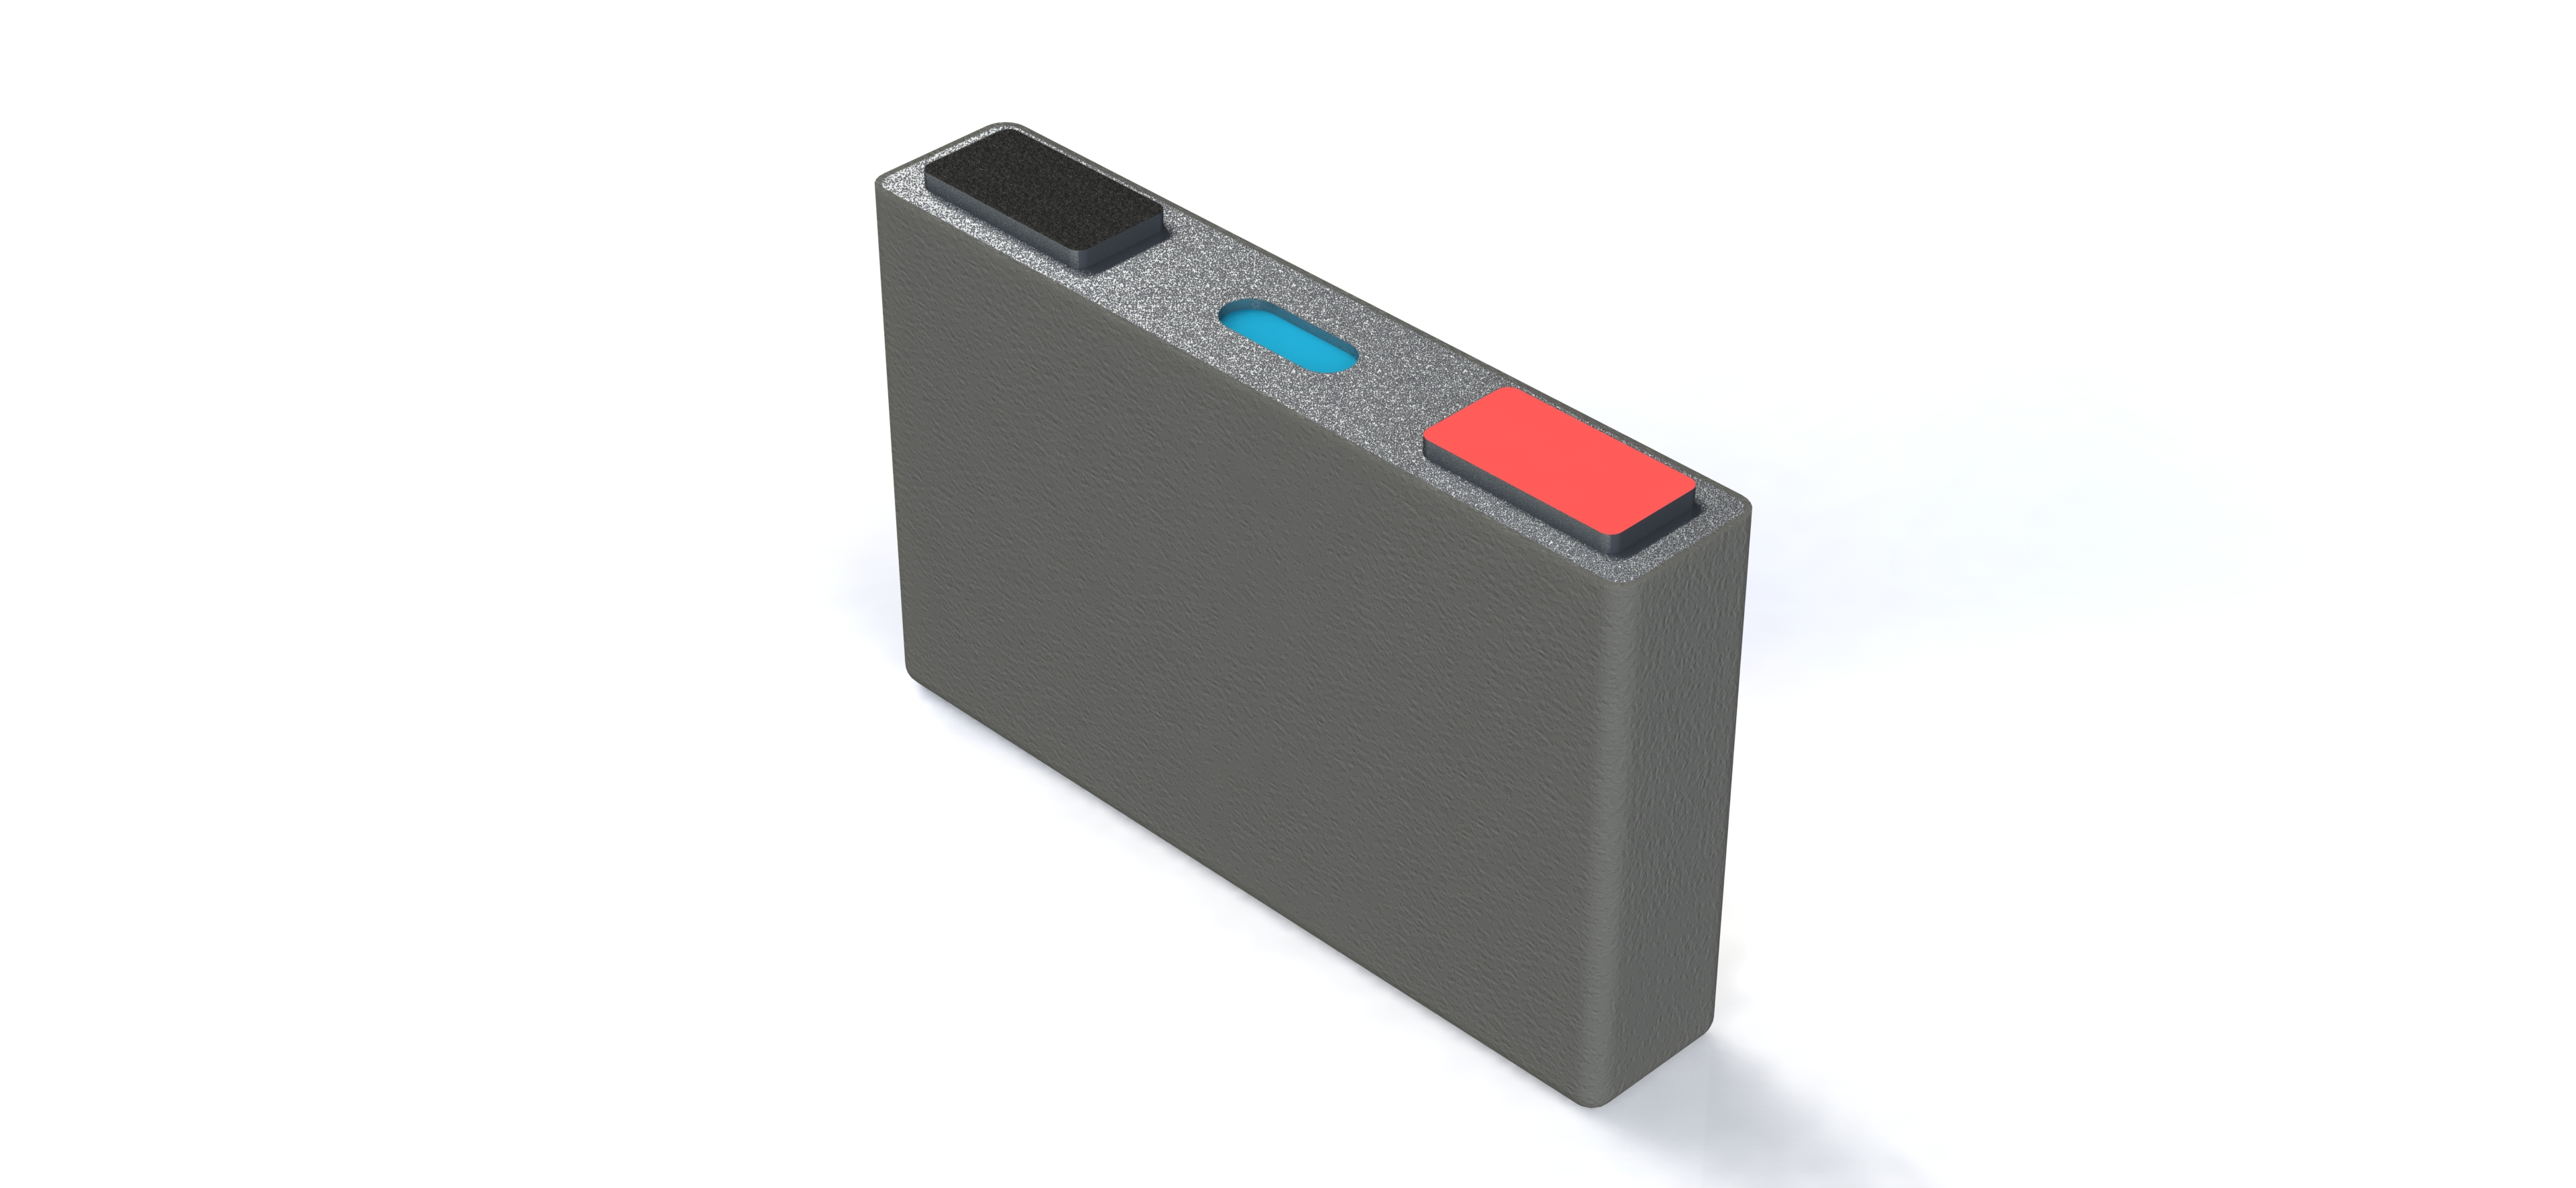
\includegraphics[width=0.9\textwidth]{figures/cell.jpg}
	\caption{电池单体设计}\label{fig:cell}
\end{figure}

在电池之间设置有电池间隔片,电池间隔片的设计阻止了电池在水平方向上的移动,并且在安装的时候可以控制间隔片的厚度来控制安装时的公差,便于手工的维修和安装,但是水平方向上安置的间隔片并没有阻止电池单体在垂直方向上的移动,在垂直方向上,本文的设计采用了一个电池箱压盖对于电池单体施加垂直压力,保证电池不会在垂直方向上发生跳动。

在电池单体之间的连接中,一般会使用铜排通过螺栓连接或者焊接与电池单体相连接,但是经过一段时间的的使用情况,螺栓通常会松动,产生危险因素,所以在目前的电动汽车电池箱设计中,一般是使用焊接方法连接电极端子 \cite{肖宁强2016插电增程式公交车电池系统设计}。

\section{电池模组级别的设计}

电池模组级别的设计主要关注的安全性问题是在模组内的电池热失控的控制和电池的压力出口点设计,电池压力出口点设计是当电池在发生热失控事件时,设计一个出口使得电池单体内部外泄的高温气流和物质沿着远离乘客的方向,或者任何会造成人员与财务损失的方向移动。这种方式会使车辆损坏和乘客安全风险最小化。在模组设计中,本文设计的压盖上有一个引导槽,可以起到泄出物质的引导作用,如图 \ref{fig:upholder} 所示。

\begin{figure}
	\centering
	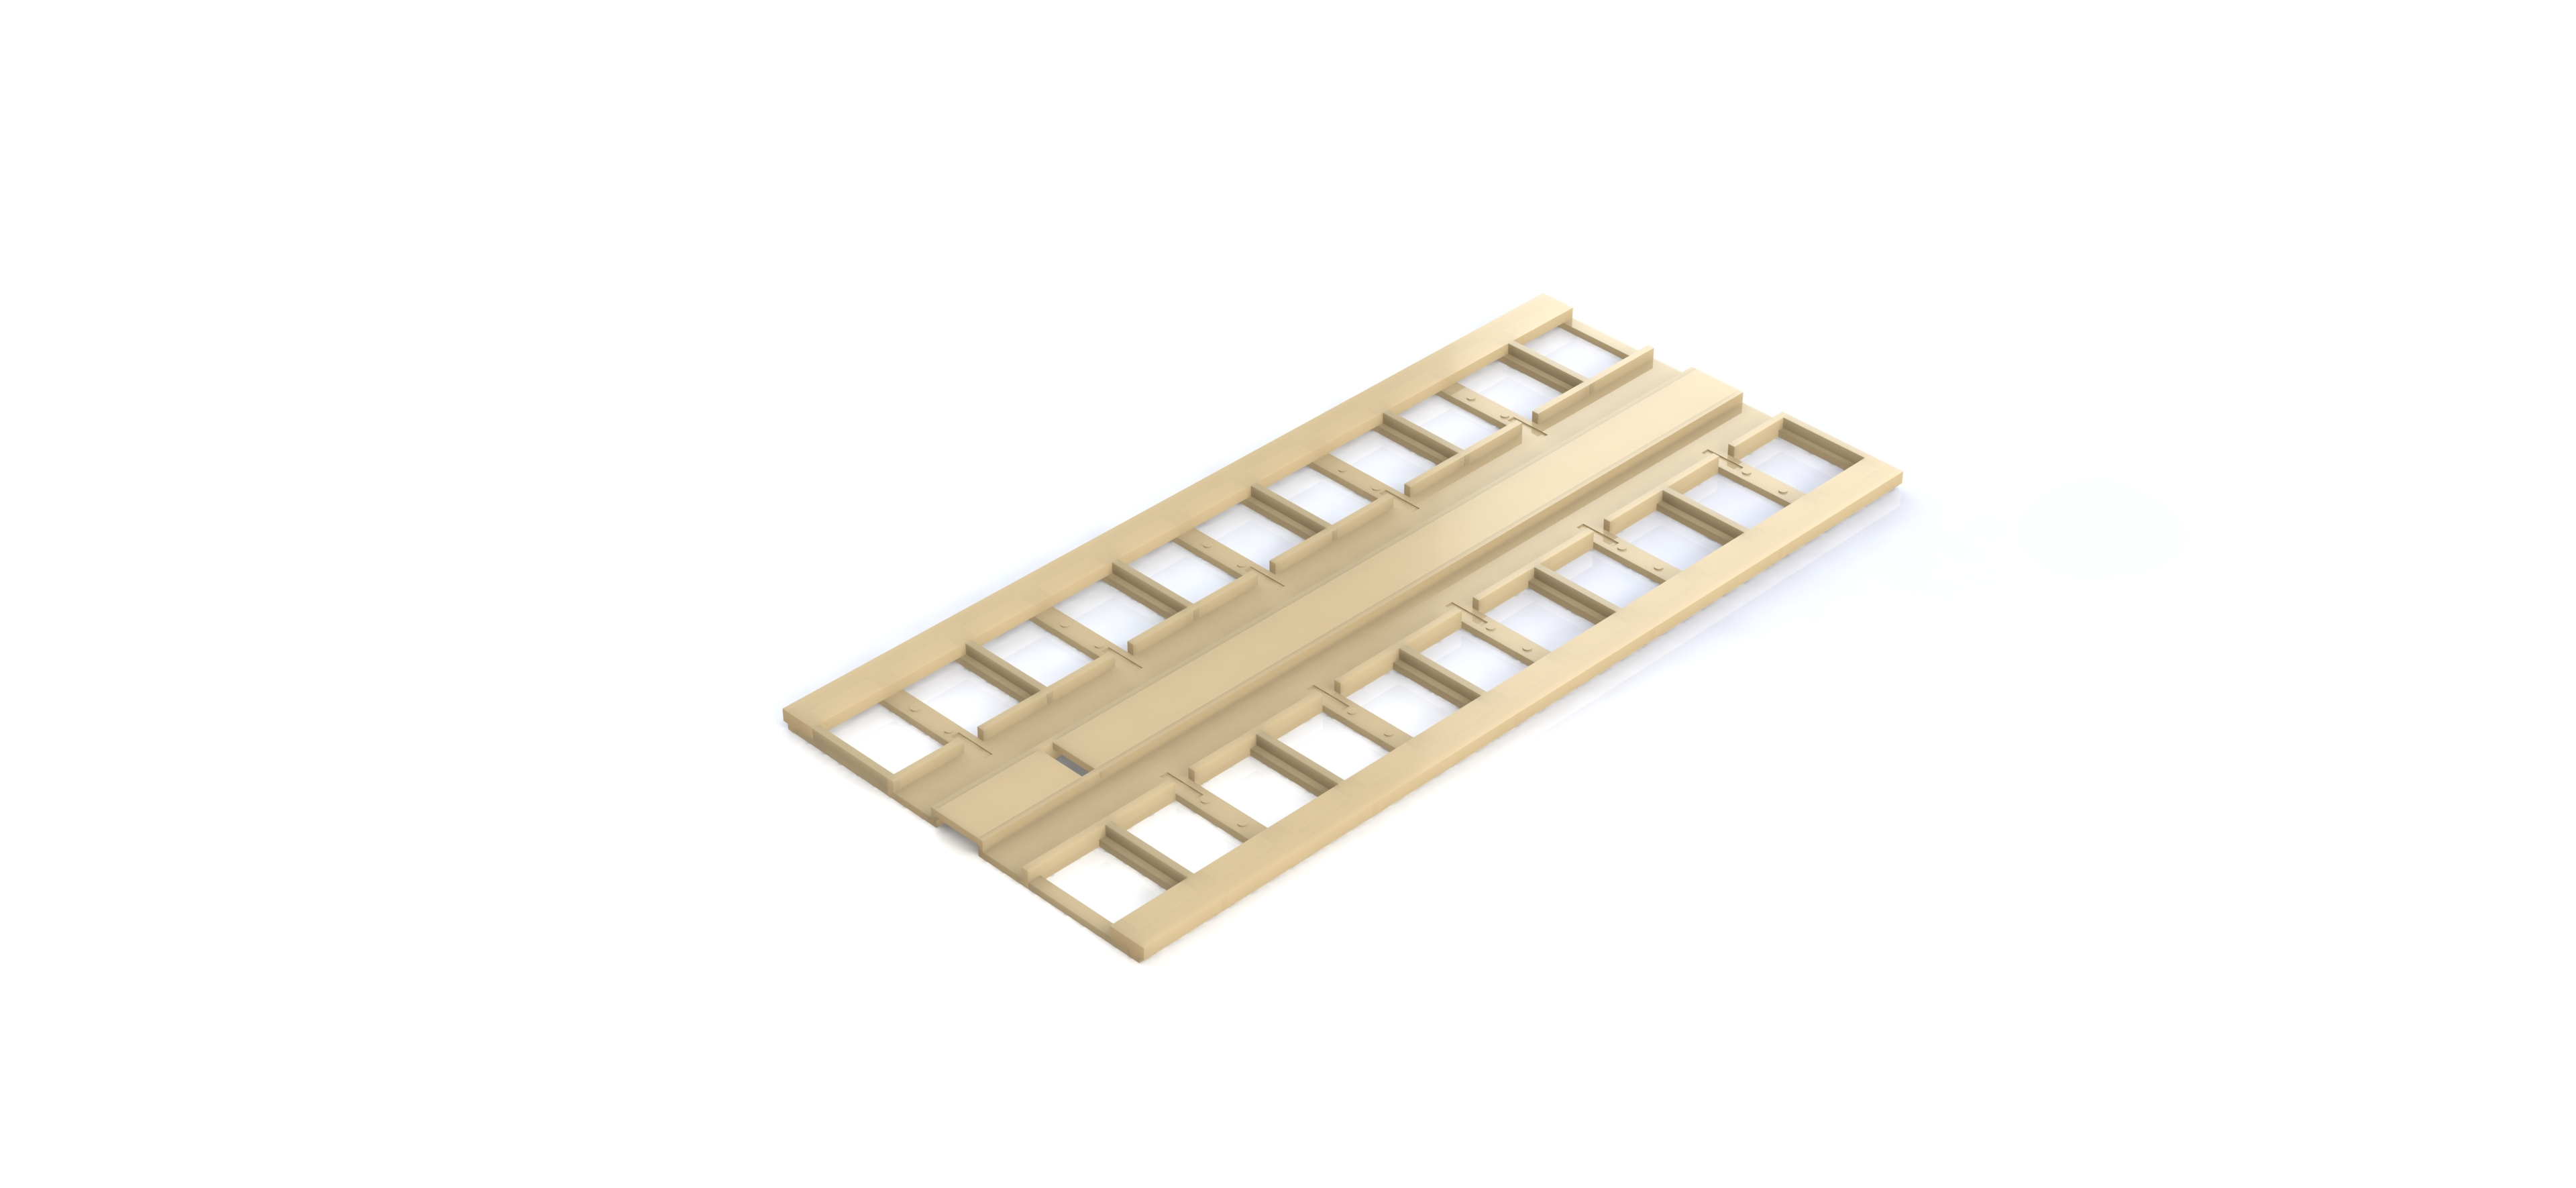
\includegraphics[width=0.9\textwidth]{figures/upholder.jpg}
	\caption{电池模组压盖设计}\label{fig:upholder}
\end{figure}

电池模组中压盖的材料为 PBT 工程塑料材质,由于 PBT 材料的耐热性较好,机械强度较大,材料的吸水性较低,尺寸稳定性好,故 PBT 材料被广泛应用于电气电子类,汽车工业类应用。每个在电池模组压盖的电池铜排下方有两个支撑住,可以起到支撑作用,由于电池连接的铜排上表面收到来自散热片压力的作用,该支撑柱可以提供支持力,避免连接铜排对电池极耳产生压力,损伤电池单体。

在电池的连接铜排上方贴有硅胶散热片,可以有效带走来自铜排的热量,并且与外壳相接触,起到绝缘和导热的作用 \cite{杨凯2014一种锂离子电池温控测试装置},选用硅胶片的原因是硅胶耐热性能较好,被广泛应用于电子器件起到导热作用,因为空气热阻较大,使用硅胶导热可以填充散热面的空气间隙,有效减小热源表面(铜排)和散热器件(外壳)之间的接触热阻。设计使用的导热硅胶片放置如图 \ref{fig:module} 所示,在该图中,在电池压盖上方已经安装好了连接铜排的和硅胶散热片。

\begin{figure}
	\centering
	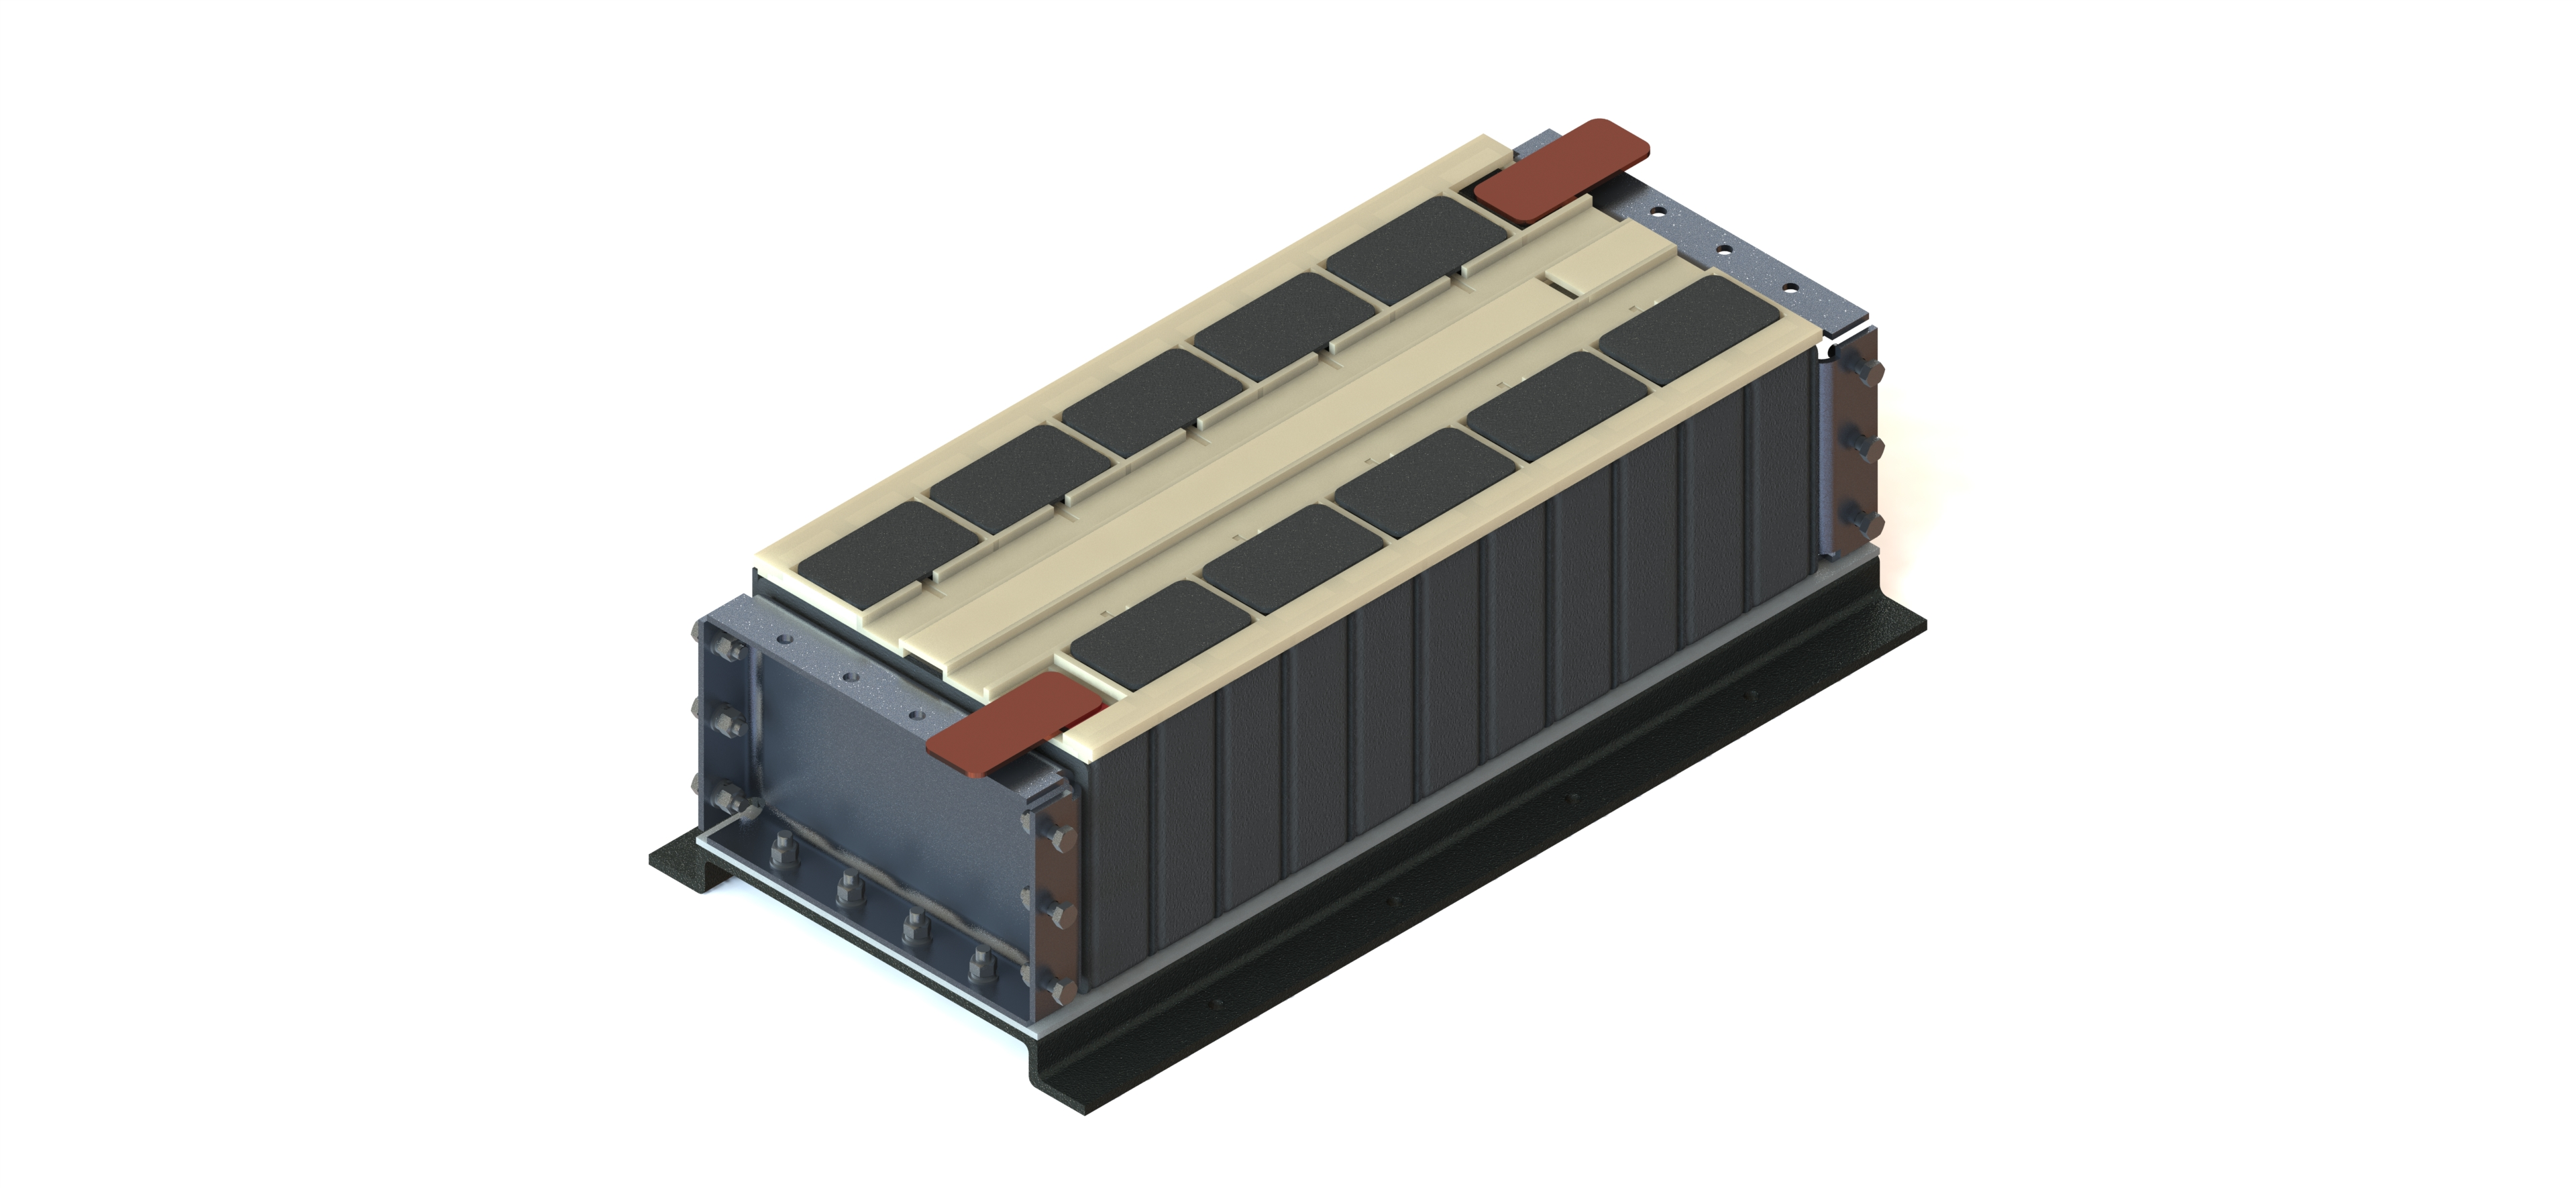
\includegraphics[width=0.9\textwidth]{figures/module.jpg}
	\caption{电池模组设计(无外壳)}\label{fig:module}
\end{figure}

电池模组的外壳为铝合金钣金材料,在外壳上方有两个凹槽,在一方面用于接触下方的硅胶散热片,将热量导出,在电池外壳该凹槽的上方可以安装水冷装置,带走热量。在电池模组的下方有漏网和凹槽,当电池发生漏液现象,漏出的液体会通过漏网流出,不会在电池模组内存留,以防止产生安全事故。含有铝合金外壳的完整的电池模组模型如图 \ref{fig:module2} 所示。

\begin{figure}
	\centering
	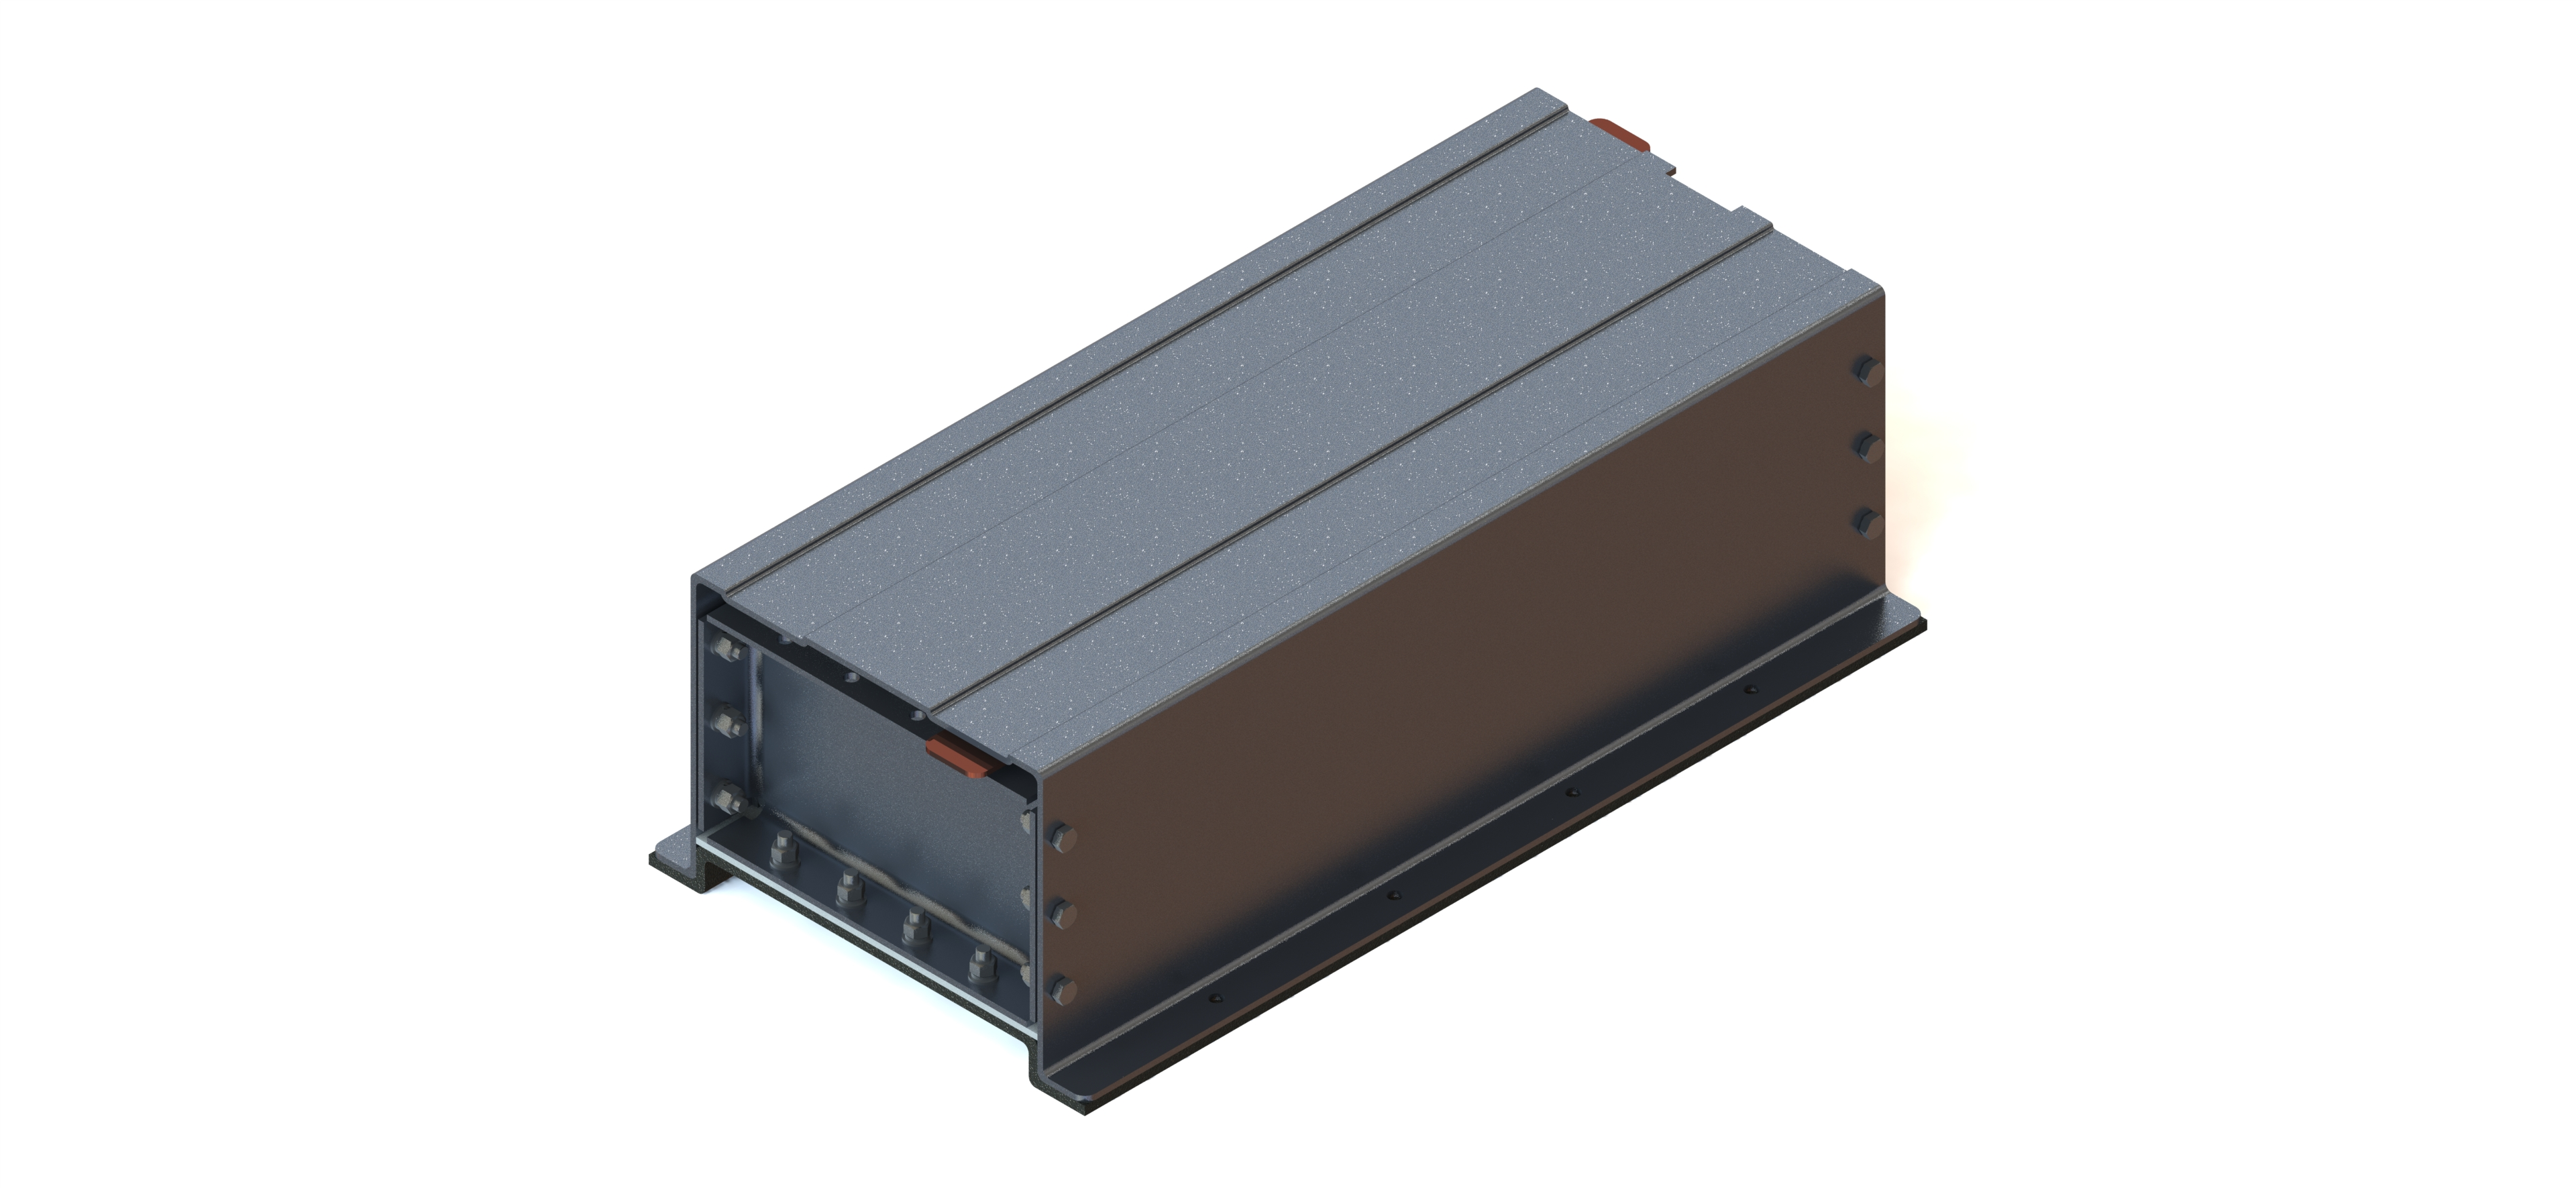
\includegraphics[width=0.9\textwidth]{figures/module2.jpg}
	\caption{电池模组设计(含外壳)}\label{fig:module2}
\end{figure}

\section{整体安装部分设计}
当考虑到电池箱与车体的连接部分,就不得不考虑车身振动和力的传递过程。当车辆在高速路以高速运行时,车辆会产生低频率的连续垂直振动输入;而当车辆运行在不平坦的道路上运行的时候,会产生冲击;当车辆起步或者转弯的时候,车辆会产生侧向加速度,而对于电池箱来说,会产生侧向力。

在美国专利 8642204 中提供了一种电池组安装框架的设计方案 \cite{BatteryManagementSystemUsedinElectricVehicles},它利用中空件结构接触电池组的下表面,并提供振动衰减的作用,在本文的设计中借鉴了该设计,使用了阻尼材料替代了专利中的结构,在电池箱的安装框架下方放置弹性阻尼橡胶板,以此来避免振动对于电池箱的影响。

在设计安装框架的时候,主要的问题是电池模组的安置问题,本文的设计参考了美国专利 8561743 中的设计方案,其设计了一种适合厂商修改电池模组数量的安装框架,并在不同的电池模组数量条件下,都能够保证电池箱的重量均匀分布,和较低的重心。本文使用了矩形的安装框架,安装框架被一根中梁等面积地分成两部分,在这两部分中,分别放置电池模组,电池模组的短边沿着车辆的纵向,长边沿着车辆的横向方向。这种电池模组的摆放方法会使电池箱的重量分布均匀,且安装稳固,如图 \ref{fig:Tray} 所示,该图展示了电池安装框架的结构。

\begin{figure}
	\centering
	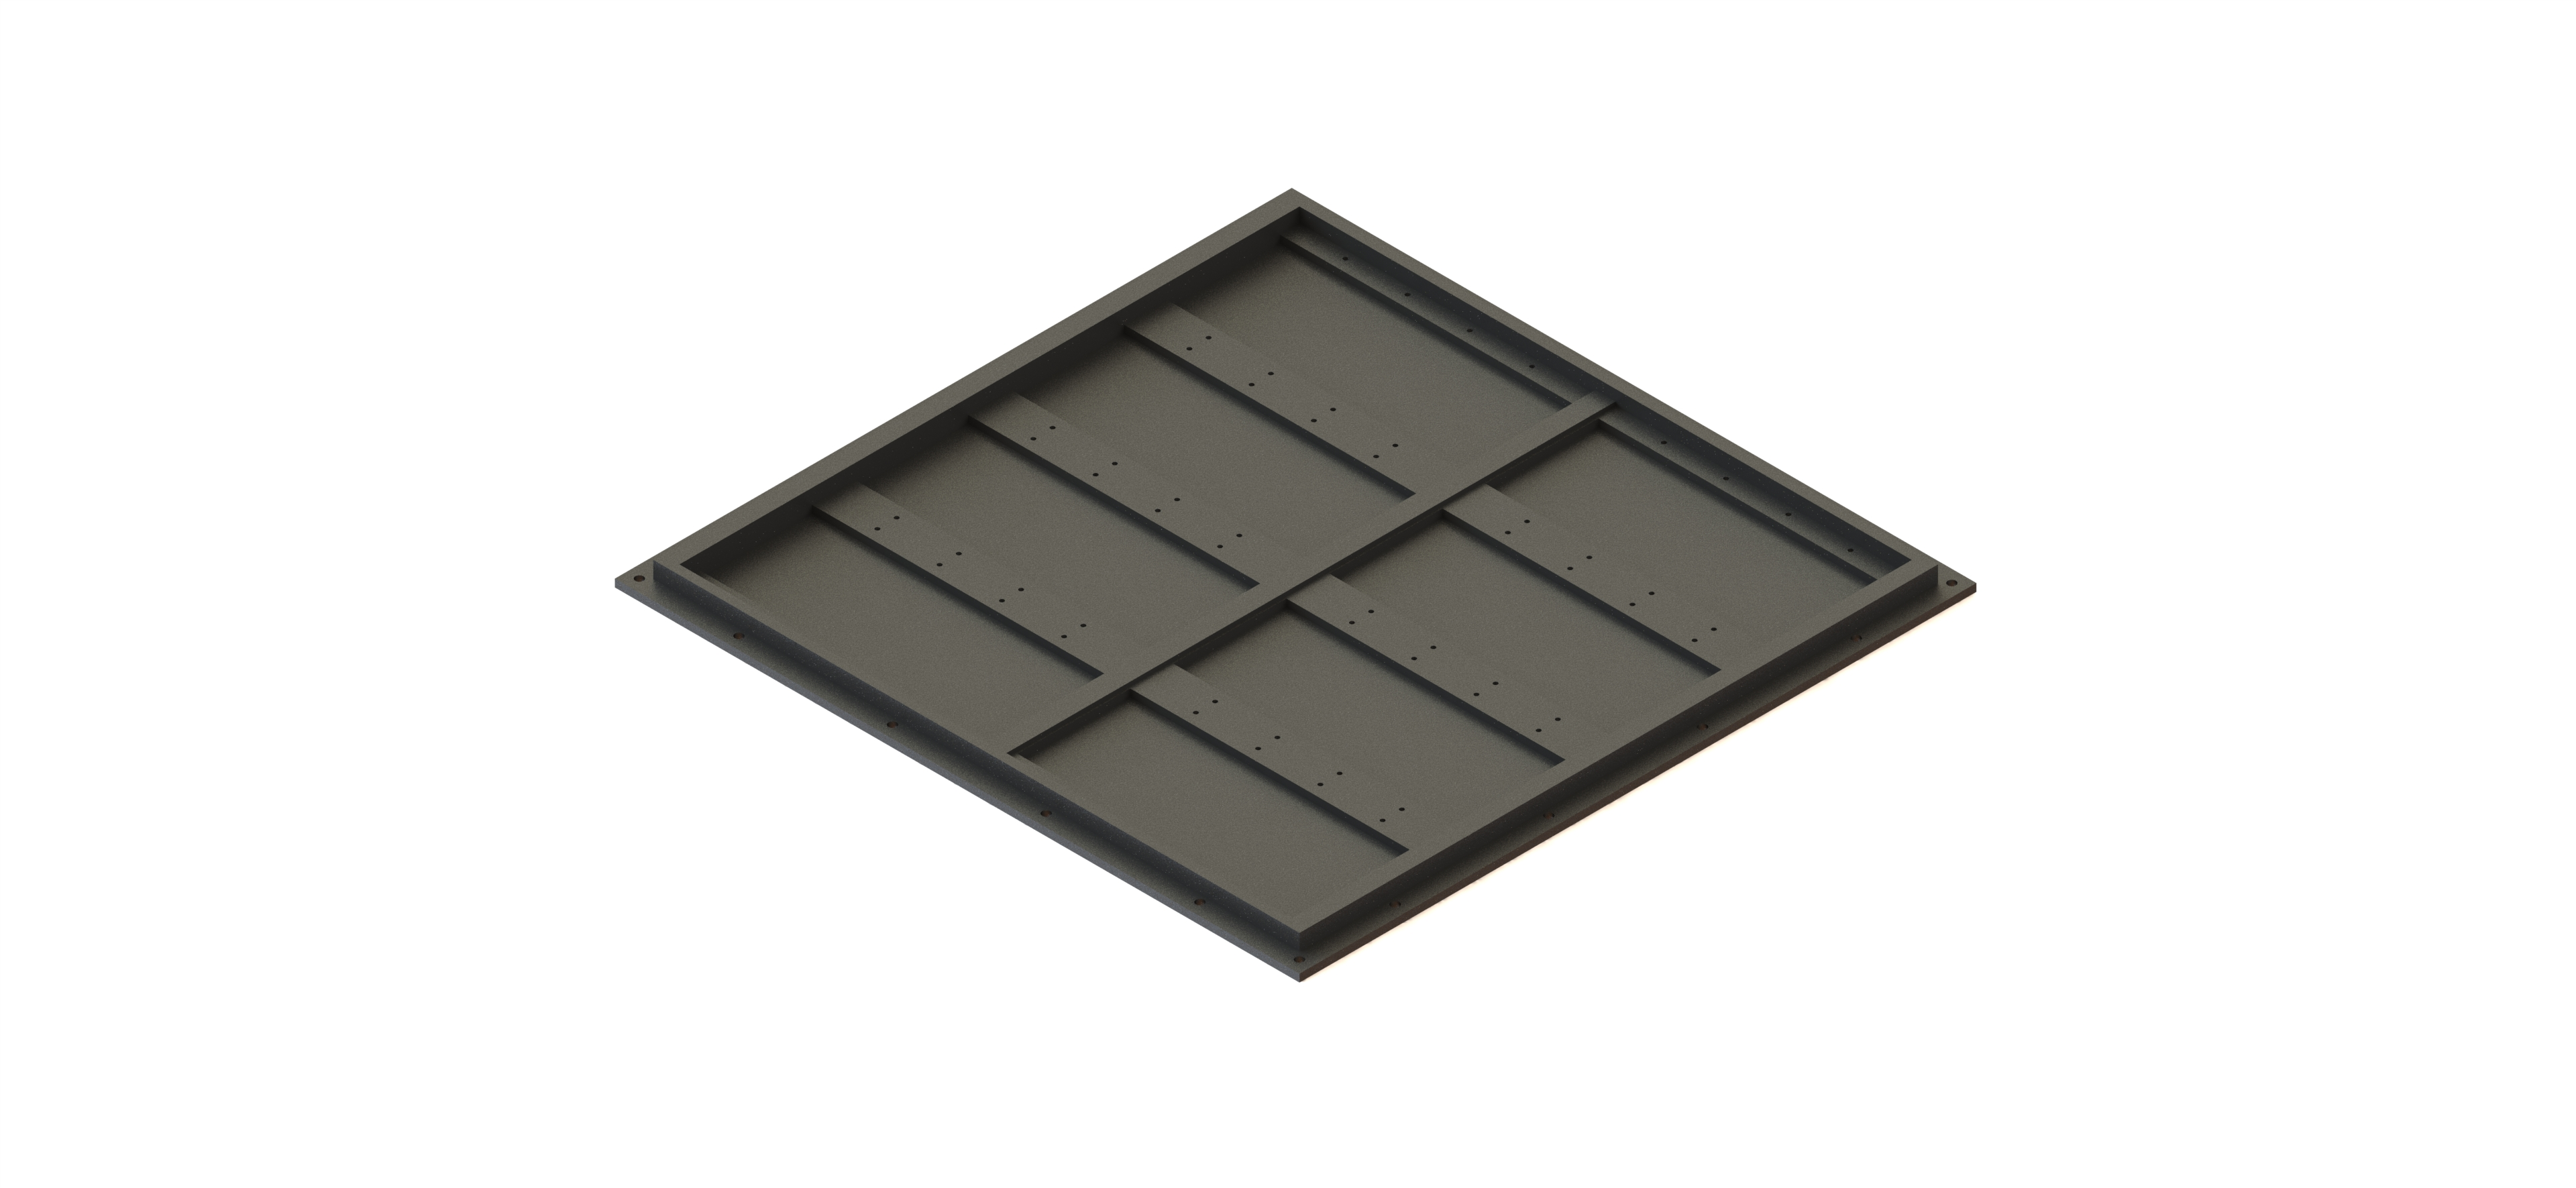
\includegraphics[width=0.9\textwidth]{figures/Tray.jpg}
	\caption{电池箱安装框架设计}\label{fig:Tray}
\end{figure}

设计最终的电池箱结构(不含上盖),如图 \ref{fig:Box} 所示,电池模组之间的连接采用铜线连接,铜线与模组之间的连接方式采用超声波焊接方式,不采用螺栓连接的方式。

\begin{figure}
	\centering
	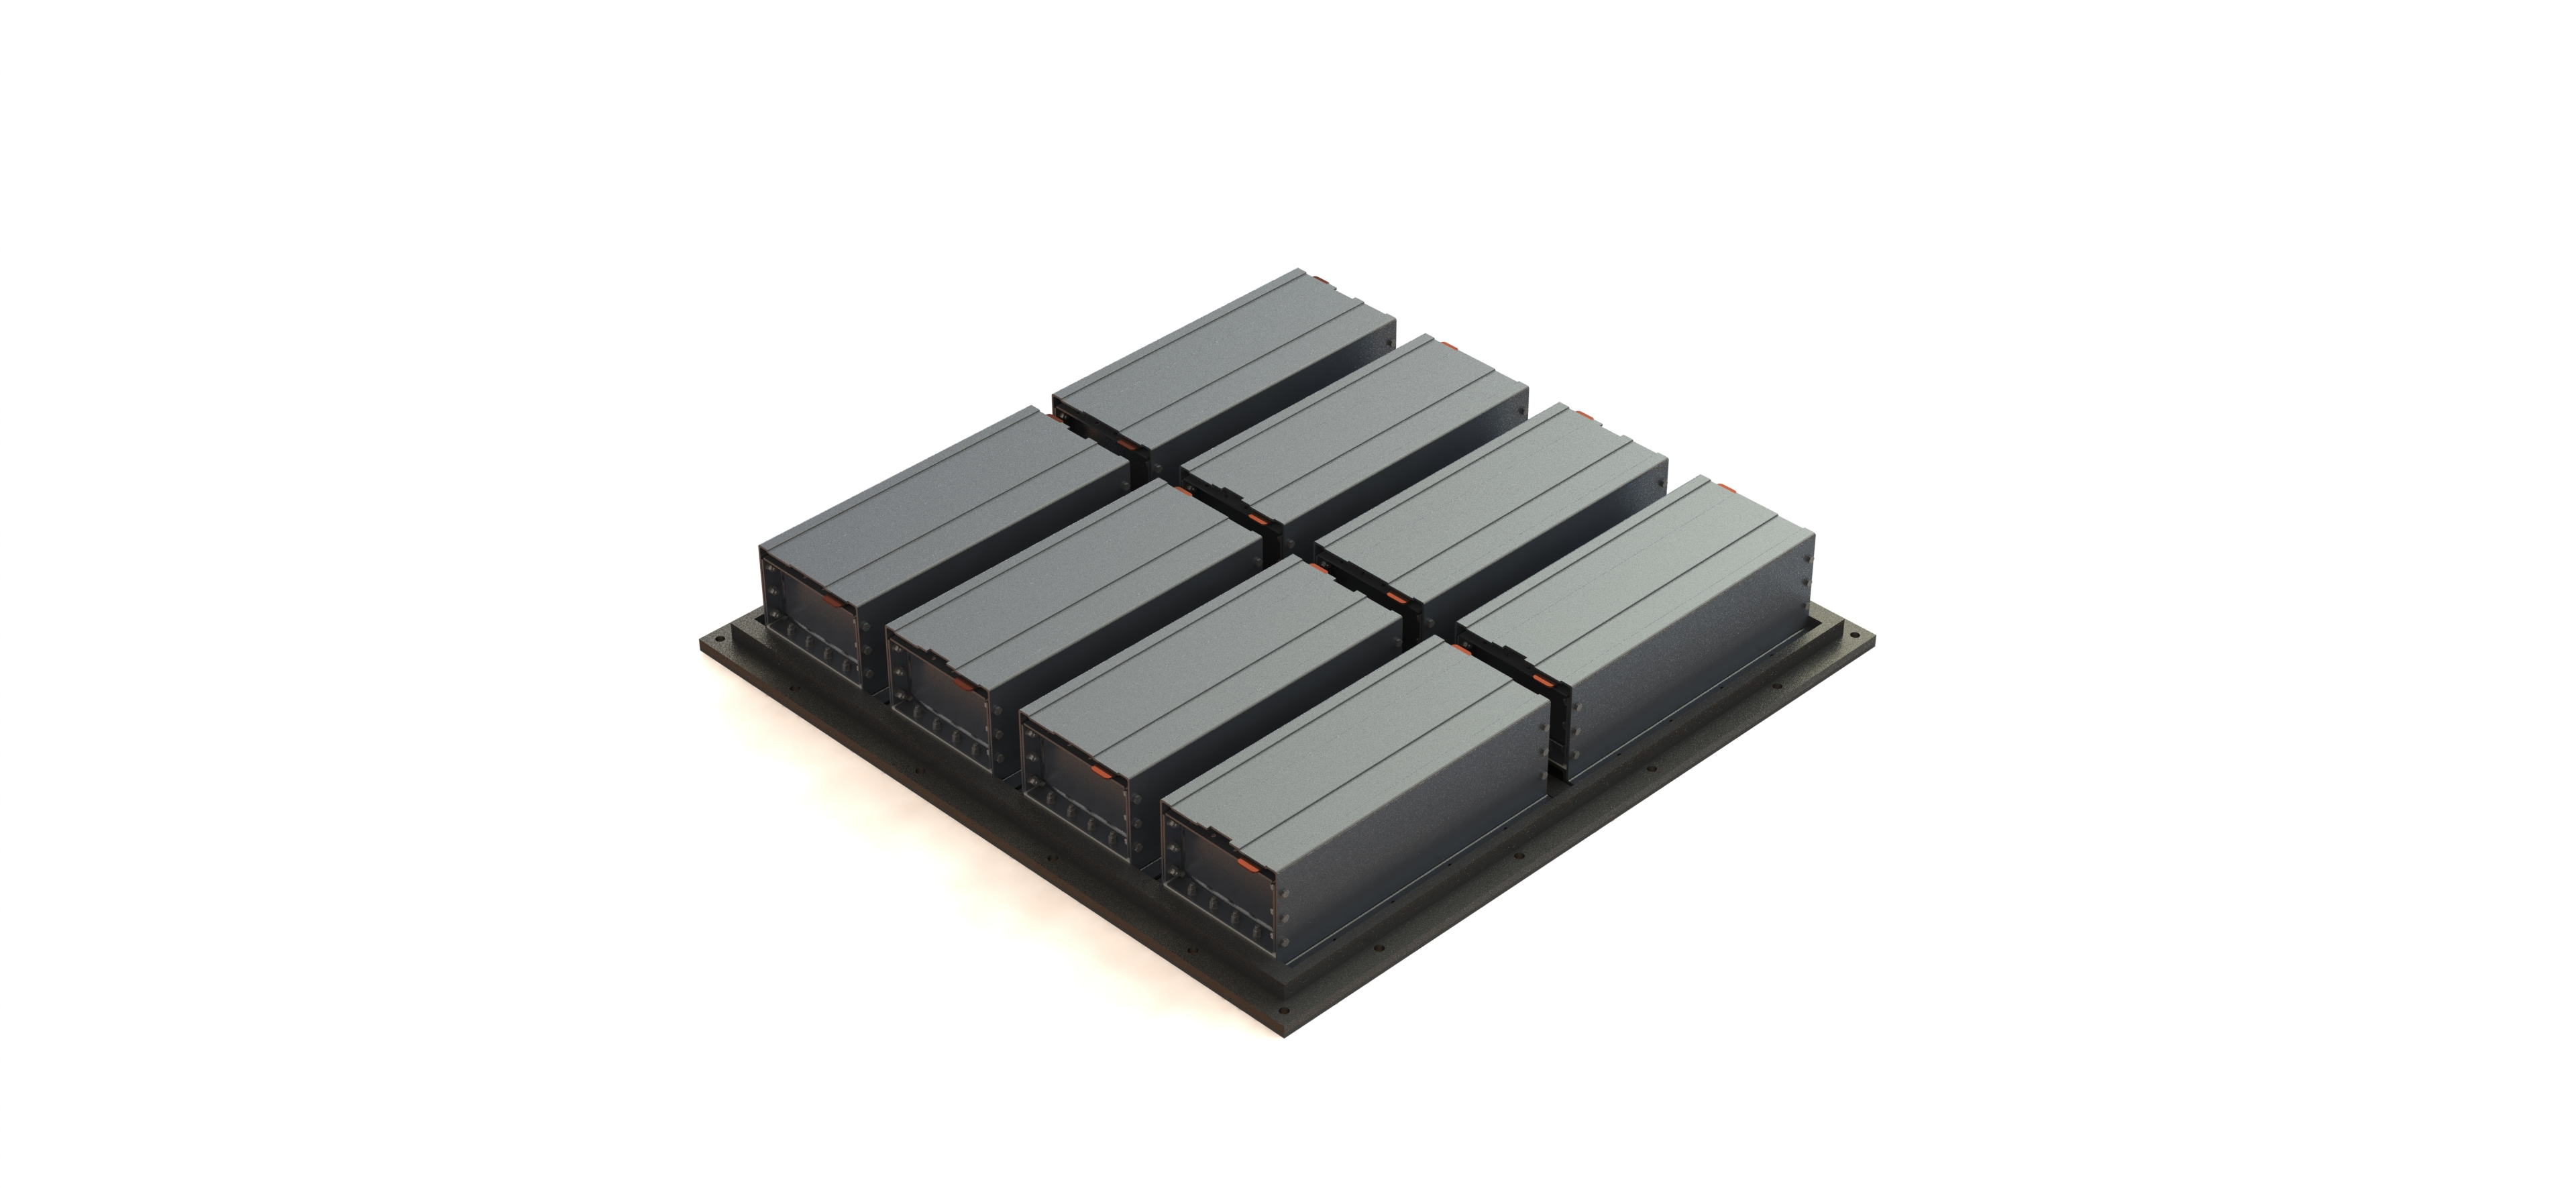
\includegraphics[width=0.9\textwidth]{figures/Box.jpg}
	\caption{电池箱整体设计}\label{fig:Box}
\end{figure}

设计完毕的电池箱机械参数如表 \ref{tab:mechinfo} 所示,表中的重量数据来自软件,是根据设计时采用的材料进行计算得到的重量值。

\begin{table}
	\centering
	\caption{电池箱机械参数} \label{tab:mechinfo}
	\begin{tabular*}{0.7\textwidth}{@{\extracolsep{\fill}}cc}
		\toprule
		参数项目			&数值		 \\
		\midrule
		质量/kg	     &115  \\
		长/mm     &891  \\
		宽/mm      &881\\
		高(不含外壳)/mm     &142  \\
		\bottomrule
	\end{tabular*}
\end{table}

\subsection{热管理}
在本文的设计当中,并未设计电池箱的热管理系统,但是在第三章节设计电池模组的过程当中,给该电池箱的热管理系统的设计准备了设计的方法。

在混合动力汽车在使用纯电动模式行驶时,由于本文设计的电池箱的额定功率和实际的驾驶功率相接近,在车辆日常行驶时,车辆的电池箱放电的倍率较大。传统风冷技术是根据气体对流换热方式进行电池箱的主动散热的,该方案的成本较低,在设计的时候较为简单,但是风冷散热的散热量有限,在电池箱的密集放热部位,如电芯和极耳等位置,使用风冷散热无法做到及时带走热量,这会导致电池箱内部的温度分散不均,影响电池的寿命,另外一方面,电池箱发生危险时,如电池箱发现热失控现象,风冷无法做到对于危险的控制。

而在其他的散热方案中,传统的液冷技术应用于电池箱方面会导致一些危险,如液体管路泄漏和阻塞,而且在日常的使用当中,传统液冷方案需要经常更换冷却液,否则在管路内产生沉积,而且系统的重量较大,占据空间较大。而采用固体相变技术散热的方案实现混合动力电池箱散热,因为固体相变技术较为复杂,而且目前的研究尚且不成熟,采用该方案的散热系统控制难度较大,而且该方式采用的合金散热材料无法做到良好的绝缘性。因此,本文设计中采用的散热方案是采用热管散热,通过安置在电池模组上方的热导管,及时带走箱内的热量。

热管散热是采用了液体发生气-液相态变化时生成和吸收热量的原理设计的,在热管的内部被分为三段,三段中的物质可以互相流通。第一段是蒸发段,贴着需要散热的表面,蒸发段内的液体吸收热量后蒸发汽化,通过第二段绝热段,到达第三段冷凝段,在冷凝段高温气体与外界交换热量,放出热量,冷凝成为液体流回第一段 \cite{周海阔2017基于热管技术的锂电池箱热管理系统设计与实验验证}。通过这种简单循环散热机制,可以做到较好的热传导速率,并且体积较小,适合在混合动力电池箱内使用。

在电池模组的下方预留了一部分空间 ,可以安装用于加热使用的电阻丝,在电池管理系统中,可以通过电池箱内部的散热和加热控制,可以有效地将箱内的环境温度差异降低,保证电池的工况条件一致性,提高电池的寿命 \cite{叶欣2017电动汽车锂离子电池散热加热设计}。

\subsection{振动隔离}
在本文的计算校核中使用了一种较为简单的校核方式,也即是利用车身的加速度来计算电池箱在运动时所产生的最大加速度量的计算方式。而在实际的驾驶过程中,由于路面存在不平度频率输入,故在设计的时候需要考虑电池箱内部的连接结构和支撑结构因为振动所造成的影响,因为在驾驶过程中的电池箱瞬时振动可能会导致电池箱因此产生的加速度远远大于本文所假设的稳态加速度条件。

在之前的机械设计章节,本文对于电池箱单体的振动隔离采用的是在水平方向上的隔板吸收振动的能量,在垂直方向上使用电池模组的压盖来抑制垂直方向上的振动。而在整体的安装方面上本文参考了美国专利 8642204 中的抗振动电池箱安装框架设计,在安装电池箱的底座四周安装阻尼块来实现振动的隔离。

\section{设计校核}

在本设计中主要的校核内容被分为两类,一类是静态校核,一类是动态校核,由于电池箱与车辆底盘相连,故车辆的运行状态会影响电池箱的受力状态,仅仅考虑电池箱在静态状态下的受力状态的校核是不可靠的,因为电池箱的质量较大,在运动过程中若存在加速度,将会对电池箱连接结构产生力的作用 \cite{王文伟2016电动汽车电池箱结构随机振动疲劳分析}。

\subsection{水平方向}
在汽车行驶过程中,汽车的加速和减速会造成汽车在水平方向上存在加速度;汽车的转向过程中,汽车会产生侧向的加速度。而汽车的纵向加速度和横向加速度的大小取决于汽车的运动状态。

在这里,本文计算的汽车的纵向加速度分为两类,一类为汽车加速运行时的纵向加速度,一类是汽车踩下刹车时,汽车减速运动的加速度。在目前的技术情况下,汽车加速时的加速度一般不会超过 1G(一个重力加速度的大小),该加速度的大小相当于百公里加速时间 2.8 秒,而当汽车踩下刹车时,车辆的最大减速度也不会超过 1G(一个重力加速度的大小)。

汽车的横向加速度与车辆的转向半径和汽车的转向速度有关,由于一般汽车的质心高度较高,质心并不与路面重合,在汽车的横向加速度超过一定值时汽车会发生侧翻现象,如式 \ref{equ:fanche} 所示,该式中,$a$ 为车辆的横向加速度,$m$ 为车辆的质量,$L_2$ 为车辆的轮距,$L_1$ 为车辆的质心高度,$g$ 为重力加速度。

\begin{equation}
\begin{aligned}
	\label{equ:fanche}
	(m \times a)\times L_2 &> (m \times g) \times \frac{L_1}{2} \\
	a &> \frac{g\times L_1}{2 \times L_2}
\end{aligned}
\end{equation}

根据一般车辆的数据带入计算,车辆发生侧翻时的最大加速度一般不超过 2G,也就是说,车辆在正常行驶的时候,理论的最大的横向加速度不超过 2G。

根据以上的计算过程,据此可以估计车载电池箱的最大水平加速度不超过 2G,根据这个加速度的边界值来判断电池箱的连接螺栓的强度。

电池底座上的螺栓连接采用紧螺栓连接,在安装的时候需要拧紧螺栓。当安装完毕的时候,螺栓的螺纹部分受到的力分为两类,一类是在安装时候施加的预紧力的 $F_t$ 产生的拉伸应力的作用,还有一类是因为在螺纹接合面处由存在的螺纹副阻力矩 $T_1$ 而产生的扭转切应力。

根据计算公式,该类型(紧螺栓连接)的螺栓在危险截面存在的拉伸应力的大小为:

\begin{equation}
	\sigma = \frac{F'}{\frac{\pi}{4}d_1^2}
\end{equation}

该类型(紧螺栓连接)螺栓危险截面的扭转切应力为:

\begin{equation}
	\tau=\frac{T_1}{W}=\frac{F'tan(\lambda+\rho_v)\frac{d_2}{2}}{\frac{\pi}{16}d_1^3}=tan(\lambda+\rho_v)\cdot \frac{2d_2}{d_1} \cdot \frac{F'}{\frac{\pi}{4}d_1^2}
\end{equation}

式中的 $T_1$ 为电池箱螺栓的扭转力矩,$W$ 为螺栓抗扭截面系数,$F'$ 为螺栓的预紧力,$\lambda$ 为电池箱螺栓的螺纹升角,$\rho_v$ 为电池箱螺栓的当量摩擦角,$d_2$ 为电池箱螺栓的螺纹中径,$d_1$ 为电池箱螺栓的小径。本文使用的是常用的 M10 型号 GB 钢制普通螺栓,带入 $tan\rho_v \approx 0.17$,$\frac{d_2}{d_1} \approx 1.04 ~ 1.08$,$tan\lambda \approx 0.05$ 代入得到:

\begin{equation}
	\tau \approx 0.5 \sigma
\end{equation}

由于螺栓的材料存在塑性,根据第四强度理论来确定螺纹部分的应力:

\begin{equation}
	\label{equ:1.3}
	\sigma_{ca}= \sqrt{\sigma^2+3\tau^3}=\sqrt{\sigma^2+3(0.5\sigma)^2}=1.3 \sigma
\end{equation}

可以看出,虽然对于本文使用的螺栓受到了拉伸力和扭转力的作用,但是在计算的时候仍可以按照纯拉伸的螺栓来计算强度,在计算中,仅仅需要将所受到的拉力,在电池箱中,拉力即为预紧力,增大 $30\%$,就足以包括扭转的影响。

\begin{figure}
	\centering
	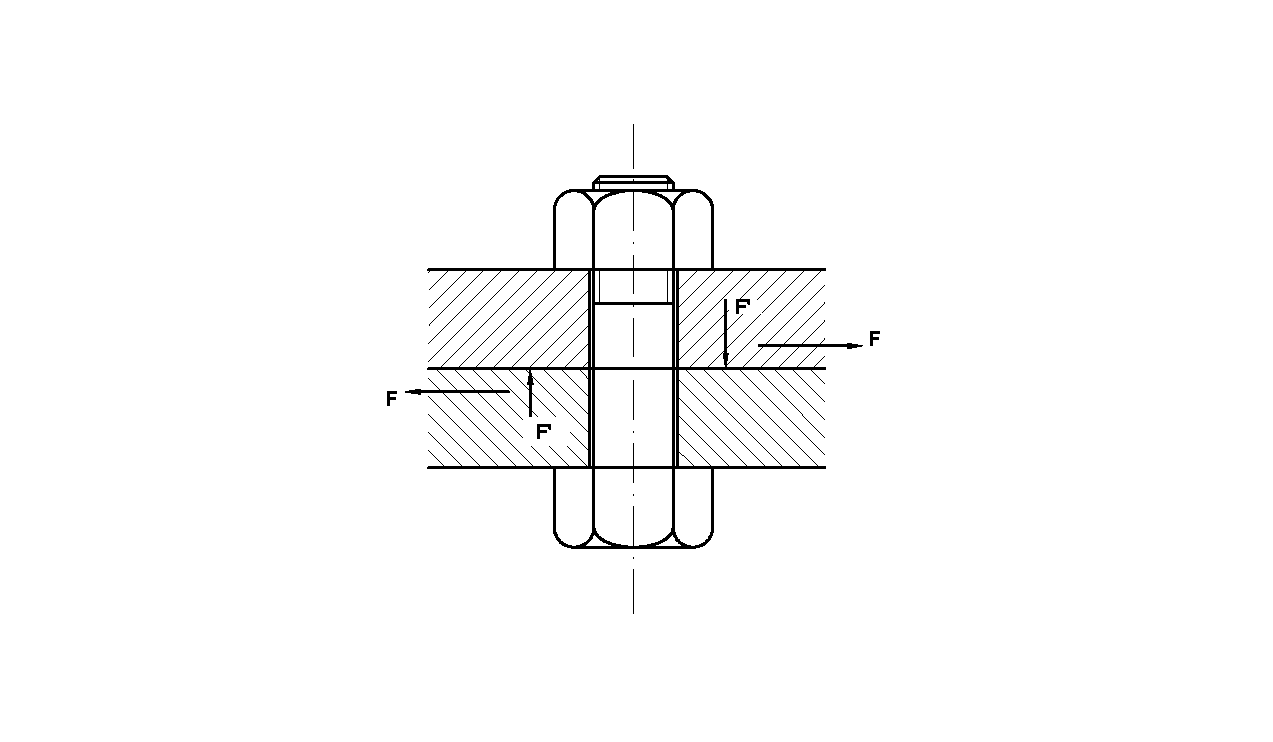
\includegraphics[width=0.9\textwidth]{figures/jiaohe-Model.eps}
	\caption{电池箱安装框架螺栓连接受力模型}\label{fig:jiaohe}
\end{figure}

如图 \ref{fig:jiaohe} 所示的螺栓连接为电池箱底座螺栓连接的模型,在运动的过程中,螺栓仅仅受到剪切力的作用,由于螺栓存在预紧力,所以在连接面产生了摩擦力来抵抗工作载荷,在这种情况下,螺栓体仅仅承受预紧力的作用,而且预紧力的大小并不收到工作载荷的影响。预紧力 $F'$ 的大小计算需要根据在螺栓结合面不产生滑移的条件决定,如式 ,式中的 $F_a$ 为电池箱因为加速度而产生的水平剪切力,$f$ 为接合面的摩擦系数,在这里为 $0.3$,$n$ 为螺栓的数量,为 20,$m$ 为结合面的数量,$m=1$,$Kn$ 为可靠性系数,$Kn=1.1$。经过计算得到的预紧力为 $F'= 413.23 N$

\begin{equation}
	F'=\frac{F_aK_n}{mnf}
\end{equation}

螺栓危险截面需要满足的强度条件如式 \ref{equ:1.3} 所示,经过计算,使用普通碳钢螺栓,材料为 Q235,查表得到其 $R_{eL}=240 \mathrm{MPa}$。选用的螺栓的直径范围为 $d=16~30 mm$,不控制预紧力且工作在变载条件下的安全系数 $S=6.5$。

\begin{equation}
	[\sigma]=\frac{R_{eL}}{[S]}=\frac{240}{6.5}=37 \mathrm{MPa}
\end{equation}

\begin{equation}
	d_1 \geq \sqrt{\frac{5.2F'}{\pi[\sigma]}}=\sqrt{\frac{5.2 \times 413.23}{3.14 \times 37}}=18.4 mm
\end{equation}

由计算得到的电池箱安装框架的螺栓直径应在 $d_1 \geq 18.4 mm $ 以上,故选择的螺栓为 M20 螺栓。

同理,根据以上的计算过程,在电池箱内安装的电池模组的安装螺栓的直径范围为:



\begin{equation}
\begin{aligned}
	F'&=\frac{F_aK_n}{mnf} = 107 N \\
	d_2 &\geq \sqrt{\frac{5.2F'}{\pi[\sigma]}}=\sqrt{\frac{5.2 \times 107}{3.14 \times 37}}=4.79 mm
\end{aligned}
\end{equation}

由此得到的电池箱模组的的螺栓直径应在 $d_2 \geq 4.79 mm $ 以上,故选择的螺栓为 M5 螺栓。

\subsection{垂直方向}

在垂直方向上的校核内容为校核电池箱连接处的材料是否会被预紧力压溃,或者在安装完成后,电池箱底座某位置产生过大的挠度。由于电池箱的内部电池质量较重,故在安装完成的时候,电池箱底板需要承受所有的重量,而一般的电池安装框架只能够在电池箱的四周固定,故电池箱底板的形变和应力状态是电池箱内的危险面 \cite{王兵2014电动汽车电池箱仿真分析及设计优化}。由于电池箱为在三维空间内的物体,故受力状态较为复杂,在本文中利用了 Solidworks 中自带的有限元分析软件来分析电池箱底座的受力变形状态与材料的状态。

在分析受力的时候,将底座连接处固定在夹具上,并向电池箱内部施加压力,用来仿真电池箱在安装完毕的时候,由于内部电池模组对于电池箱安装框架的压力,在计算的时候,力被均匀加载在电池安装框架上。

\subsubsection{应力分析}

在分析应力的时候,采用的应力分析准则为 von Mises 准则,又被称为范式等效应力。该准则综合了各个主应力的作用,被广泛用于材料的应力分析当中,范式等效应力的准则是,当在被分析材料中的某一点所在位置的点应力达到达到某一与应力状态无关的定值时,材料就发生屈服或者压溃现象,换句话说,当材料的弹性势能超过某一界限的时候,就认定材料发生了屈服现象。

对于电池箱安装框架的有限元分析过程,第一步,首先要限定电池箱的机械连接部分,在软件中使用软件提供的夹具功能将电池箱底座与车体相连接的部分固定,在校核的时候,本文认定在机械连接的部分因为已经安装有螺栓,该处已经固定在车体上不因为受到来自电池单体的压力而发生应变;第二步,在电池模组的位置加载等效电池模组对于底座压力的力,因为每个电池单体的质量为 $12 kg$,一共有 8 个模组,重力加速度为 $g=9.8m^2$,在电池箱一共施加的等效力的大小为 $940.8 N$;第三步,为了轻量化设计,电池箱底座的材料选择 1060 铝合金材质,在软件中设置零件的材料为 1060 铝合金。

使用此应力定则分析本文的电池安装框架中可以得到各点处的范式等效应力的大小值,如图 \ref{fig:yingli} 所示,在图中可以看到,材料的范式等效应力范围最大处应力为 5.42 MPa,材料的范式屈服应力值为 27.6 MPa,材料并未发生屈服。

\begin{figure}
	\centering
	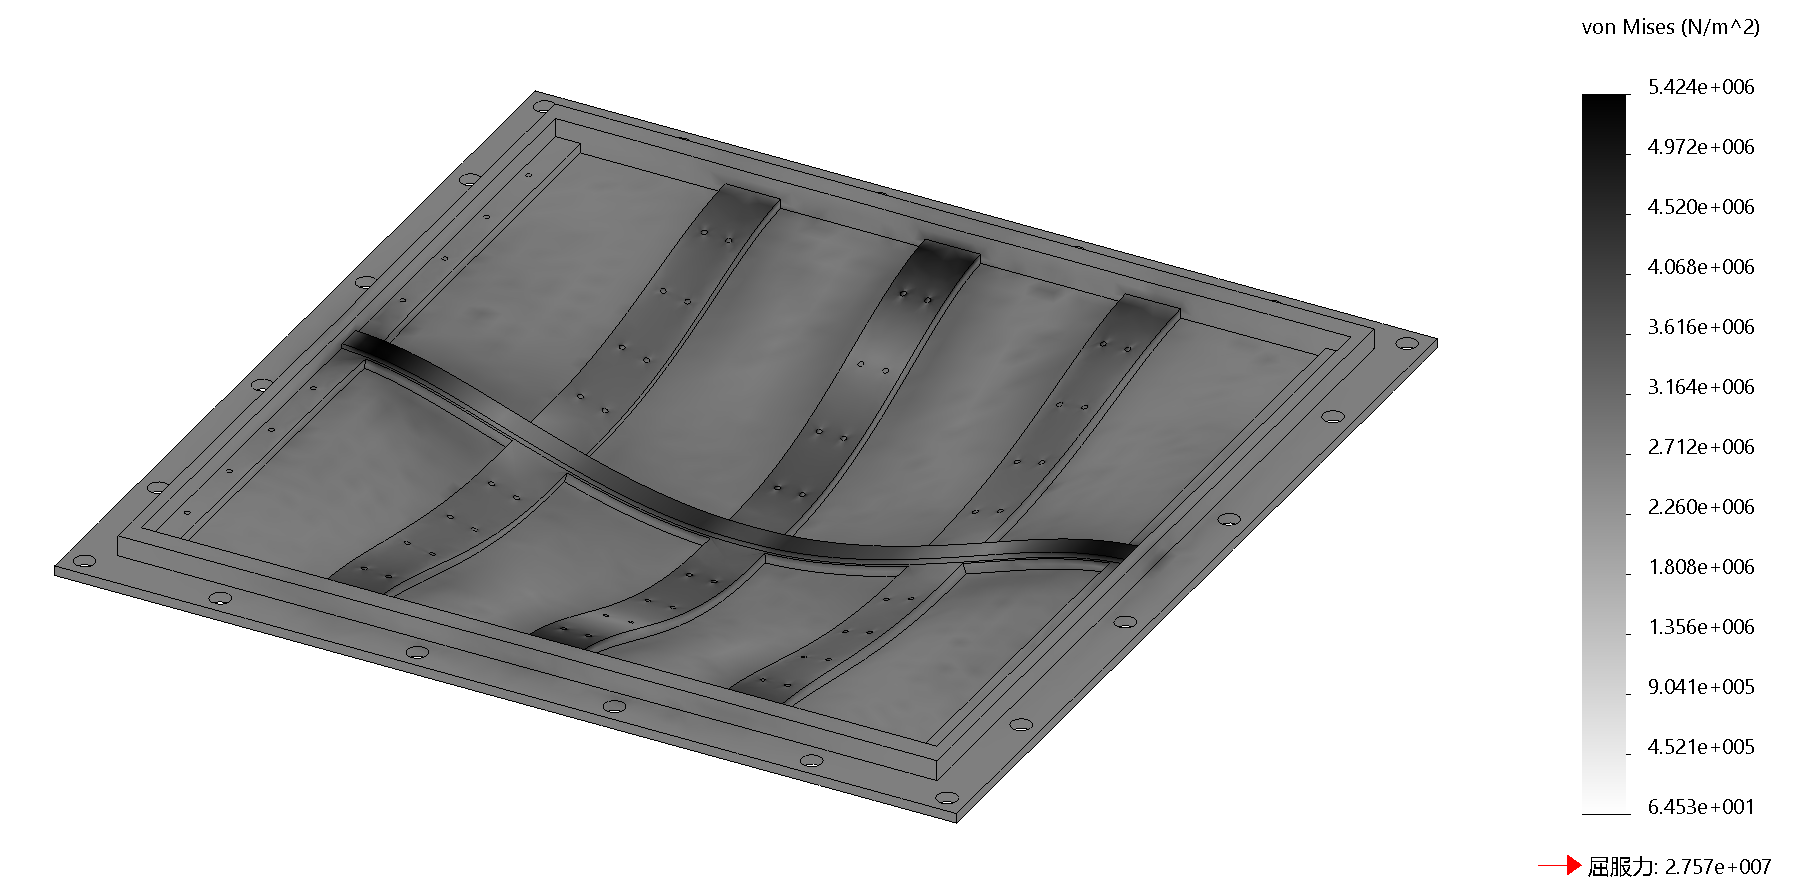
\includegraphics[width=0.9\textwidth]{figures/yingli.png}
	\caption{电池箱安装框架应力分布图(应变放大 500 倍)}\label{fig:yingli}
\end{figure}

根据 Solidworks 提供的应变分析引擎,可以得到电池箱安装框架在安装后的应变分布,如图 \ref{fig:yingbian} 所示,在电池箱底座中,最大应变量为 $0.181 mm$。

\begin{figure}
	\centering
	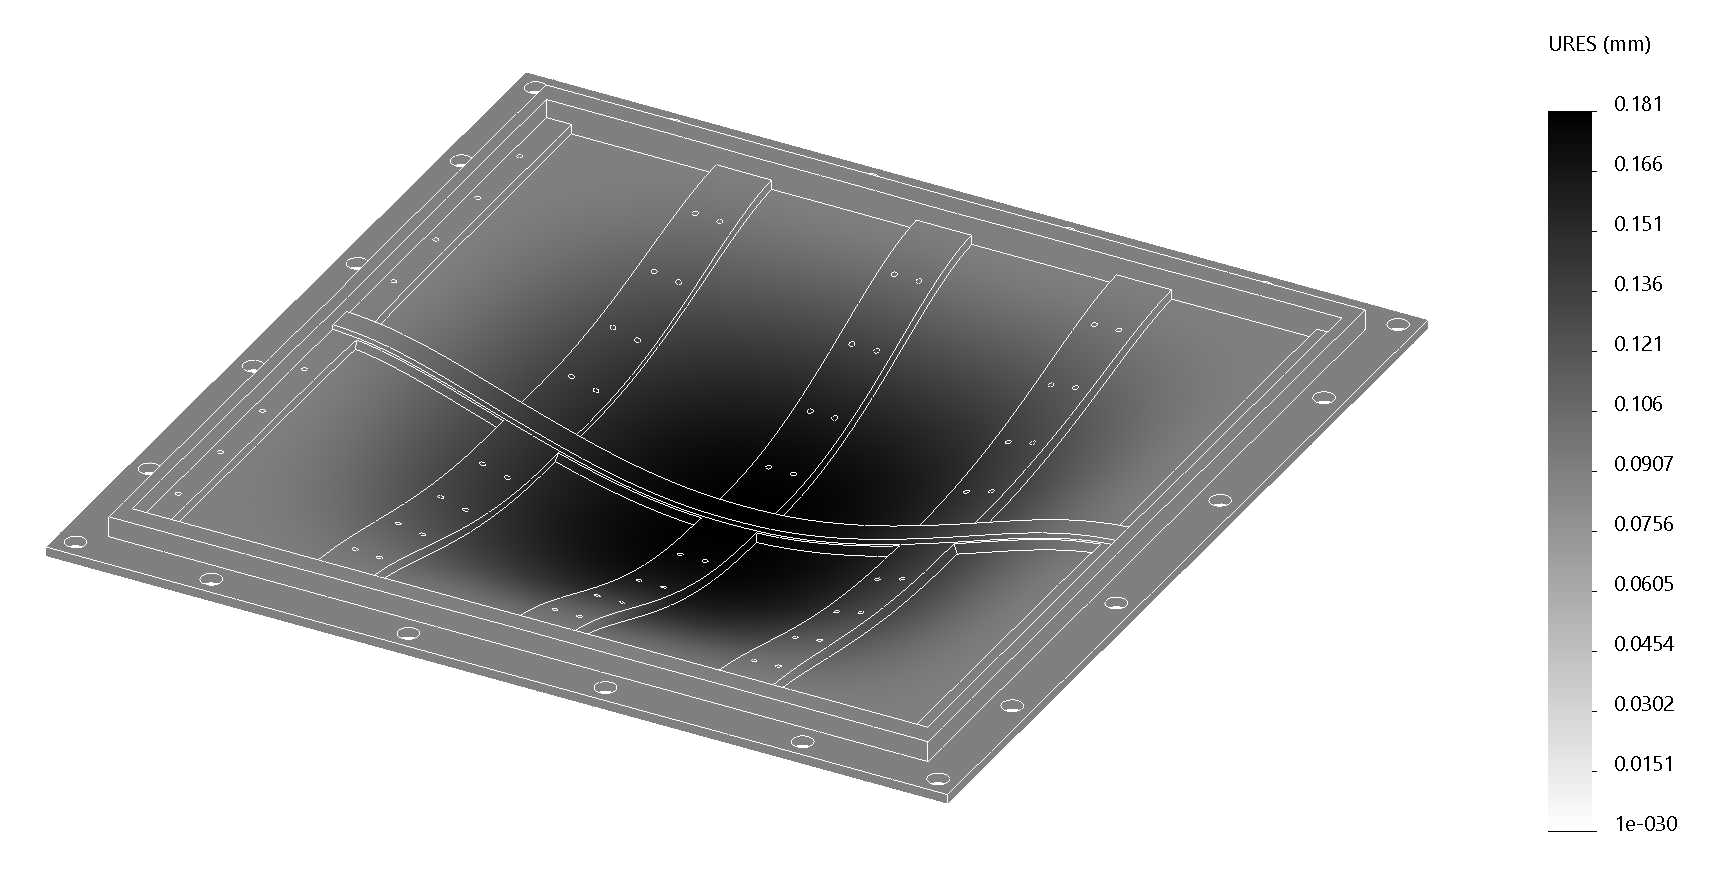
\includegraphics[width=0.9\textwidth]{figures/yingbian.png}
	\caption{电池箱安装框架应变分布图(应变放大 500 倍)}\label{fig:yingbian}
\end{figure}

根据有限元软件校核的结果,可以判断本文设计的电池箱安装框架结构符合使用要求,并且给出了在安装电池模组和在安装电池安装底座的螺栓预紧力的值。
\chapter{电池 OBD 系统设计}
\label{chap:OBD}

\section{OBD 系统简介}
在当前社会,车辆作为人们日常使用最多,普及程度最高的交通运输工具之一,已经发展成为一个拥有机械和电子技术复杂的体系,而对于汽车上存在的诸多部件,在过去,各个汽车生产商采用不同的诊断方法,而采用传统的诊断方法无法做到对于故障的及时诊断与回报,用户无法直接了解汽车是否故障,也无法判断车子的故障状态,只有将车辆送回维修厂,使用专业的诊断仪器才能够了解故障状态;在政府方面,汽车采用不同的诊断系统也无法形成一个系统化的监管制度,如何做到汽车的故障统一,系统的故障诊断的过程标准化,故障项目标准化,在这种情况下车载诊断系统,又被称作 OBD(On Board Diagnosis)系统,首先被美国提出的标准化诊断系统,被推广至今,已经成为一个统一的诊断系统,该系统会在指定的时间间隔内监控车辆的运行状态,并且通过对于来自传感器的数据进行储存,分析,诊断出是否存在故障。一旦车辆的某一个子系统或者部件产生了问题,OBD 系统就会通过内部的数据库检查故障的类型和严重程度,在某一条件符合的情况下,将会产生故障代码,储存在系统的非易失性储存其中,并且通过汽车总线发送提醒讯号(MIL 灯)通知驾驶员和汽车维修厂的维修人员。

OBD-II 与第一代的 OBD 系统相比,统一了 OBD 系统的物理接口,以及引脚,并且在物理接口处提供了给外部诊断仪器的供电的引脚,当外部的诊断仪插入后,不需要额外的供电,就可以运行,简化了诊断的过程。同时 OBD 协议也规定了一个标准的电气信号传输格式,以及传输的内容,在原有的仅能够支持故障的诊断相比,增加了实时监控车辆的运行数据的功能,虽然 OBD-II 标准的目标是提供车辆排放方面的诊断,但是目前的大多数汽车制造厂商会将 OBD 系统放置在整车网络上,使得所有的设备都能够被同时诊断故障。

一个基本的车载 OBD 系统如图 \ref{fig:OBD_structure} 所示。汽车的 MIL 灯(Malfunction Indicator Lamp)通常情况下由汽车的 VCU(整车电子控制单元)控制,在平常的适用情况下,OBD 系统将会采集来自于传感器的数据并将数据分类暂时储存,以便使用,并在同时对数据进行诊断,对于故障进行分类储存。而当系统发生故障之后,对应子系统的 OBD 系统将会上报故障给 VCU,VCU 通过已经上报的故障进行判断是否进行 MIL 灯的点亮。而在故障发生后,检测人员将会使用诊断仪读取已经储存的数据,包括故障发生时的传感器数据,时间,和故障的相关信息,在维修后通过诊断仪也可以发送指令给对应的 OBD 系统,进行储存故障信息的清除,熄灭车辆的 MIL 故障灯。

\begin{figure}
	\centering
	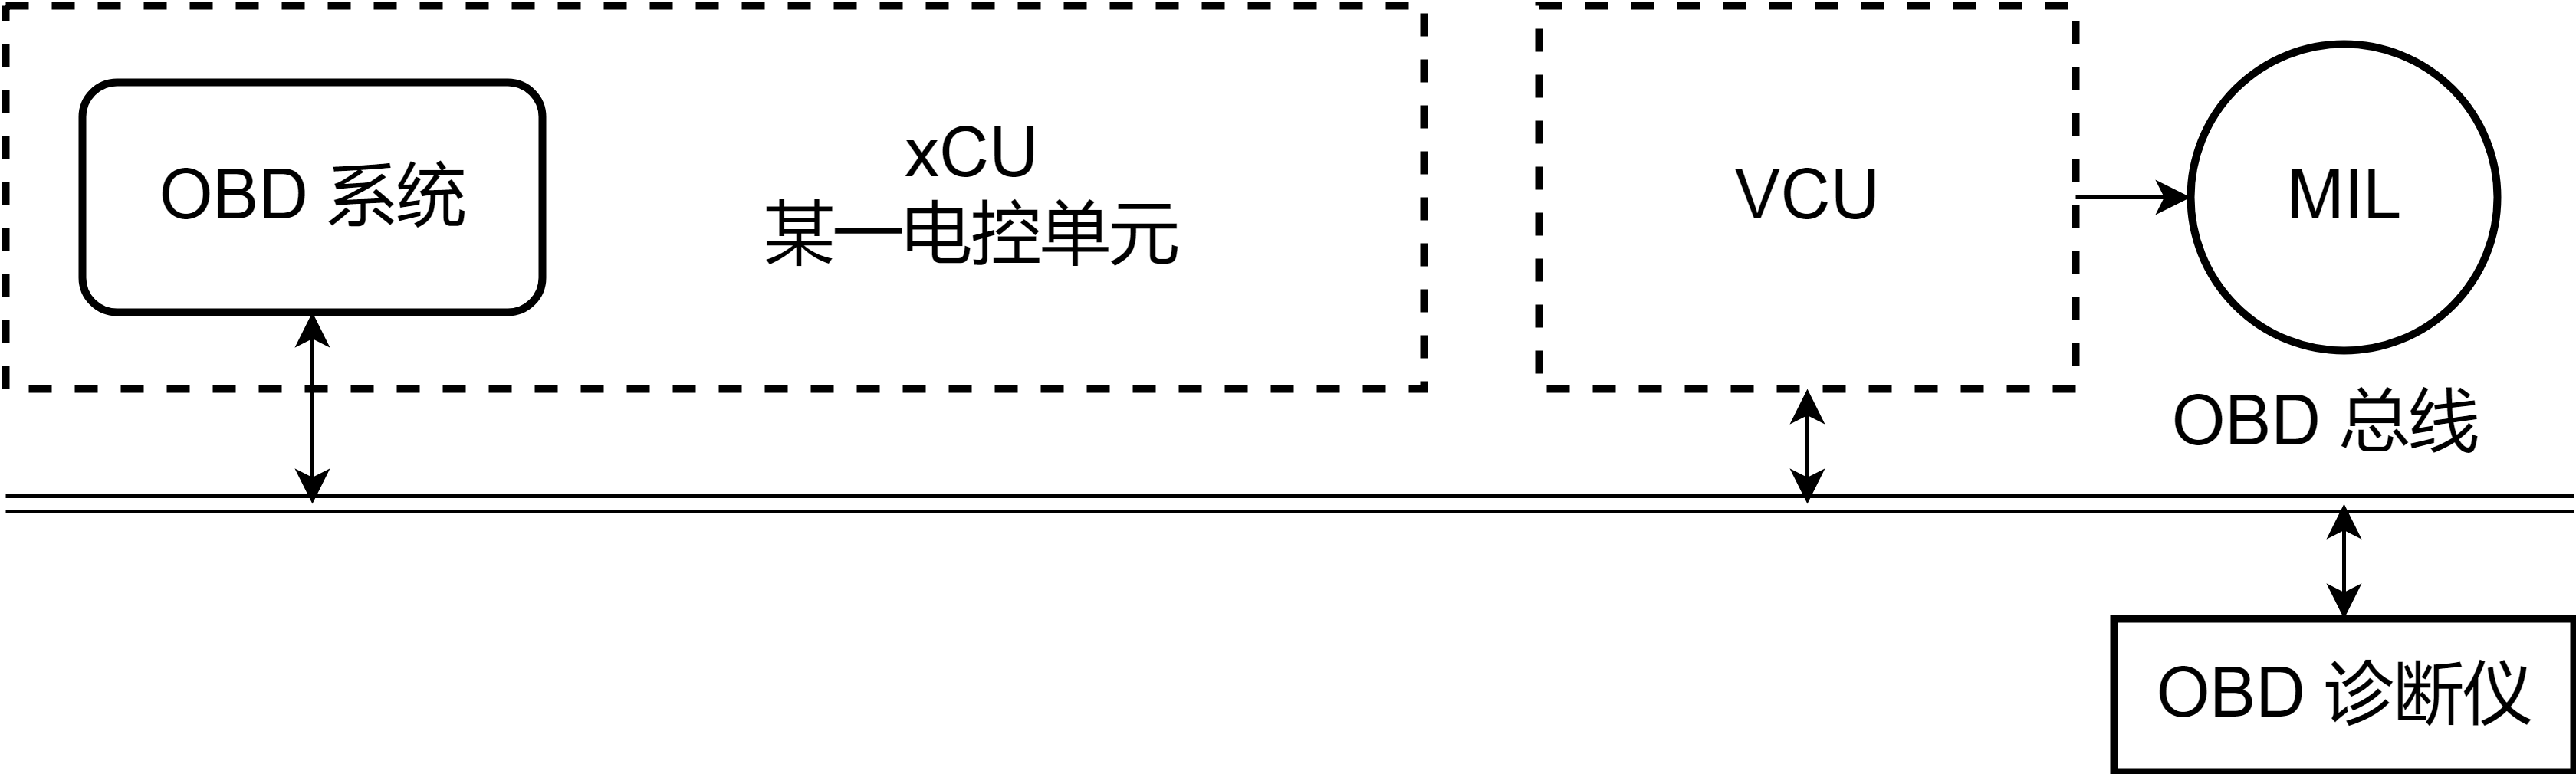
\includegraphics[width=0.7\textwidth]{figures/OBD_structure.png}
	\caption{新能源汽车的 OBD 系统结构}\label{fig:OBD_structure}
\end{figure}

随着目前的计算机技术发展,目前的车载诊断系统已经具备多种多样的功能,譬如在汽车总线之外,还能够通过多种信息传输介质来进行信息的传输,这时由于 OBD 系统仅仅规定了标准化的信息传输协议,而没有限定信息传输的介质,在未来,OBD 系统将会基于更加高速的传输介质,如以太网和蓝牙,并可以和物联网紧密结合 \cite{屠雨2016基于汽车OBD车联网的设计与实现,白东2017基于OBD的车辆信息管理平台}。而且 OBD 系统也会拥有更多更完善的功能,譬如对于故障数据的集中汇总,进行大数据分析,更加人性化的用户界面等功能,如图 \ref{fig:OBD_structure} 所示。

\begin{figure}
	\centering
	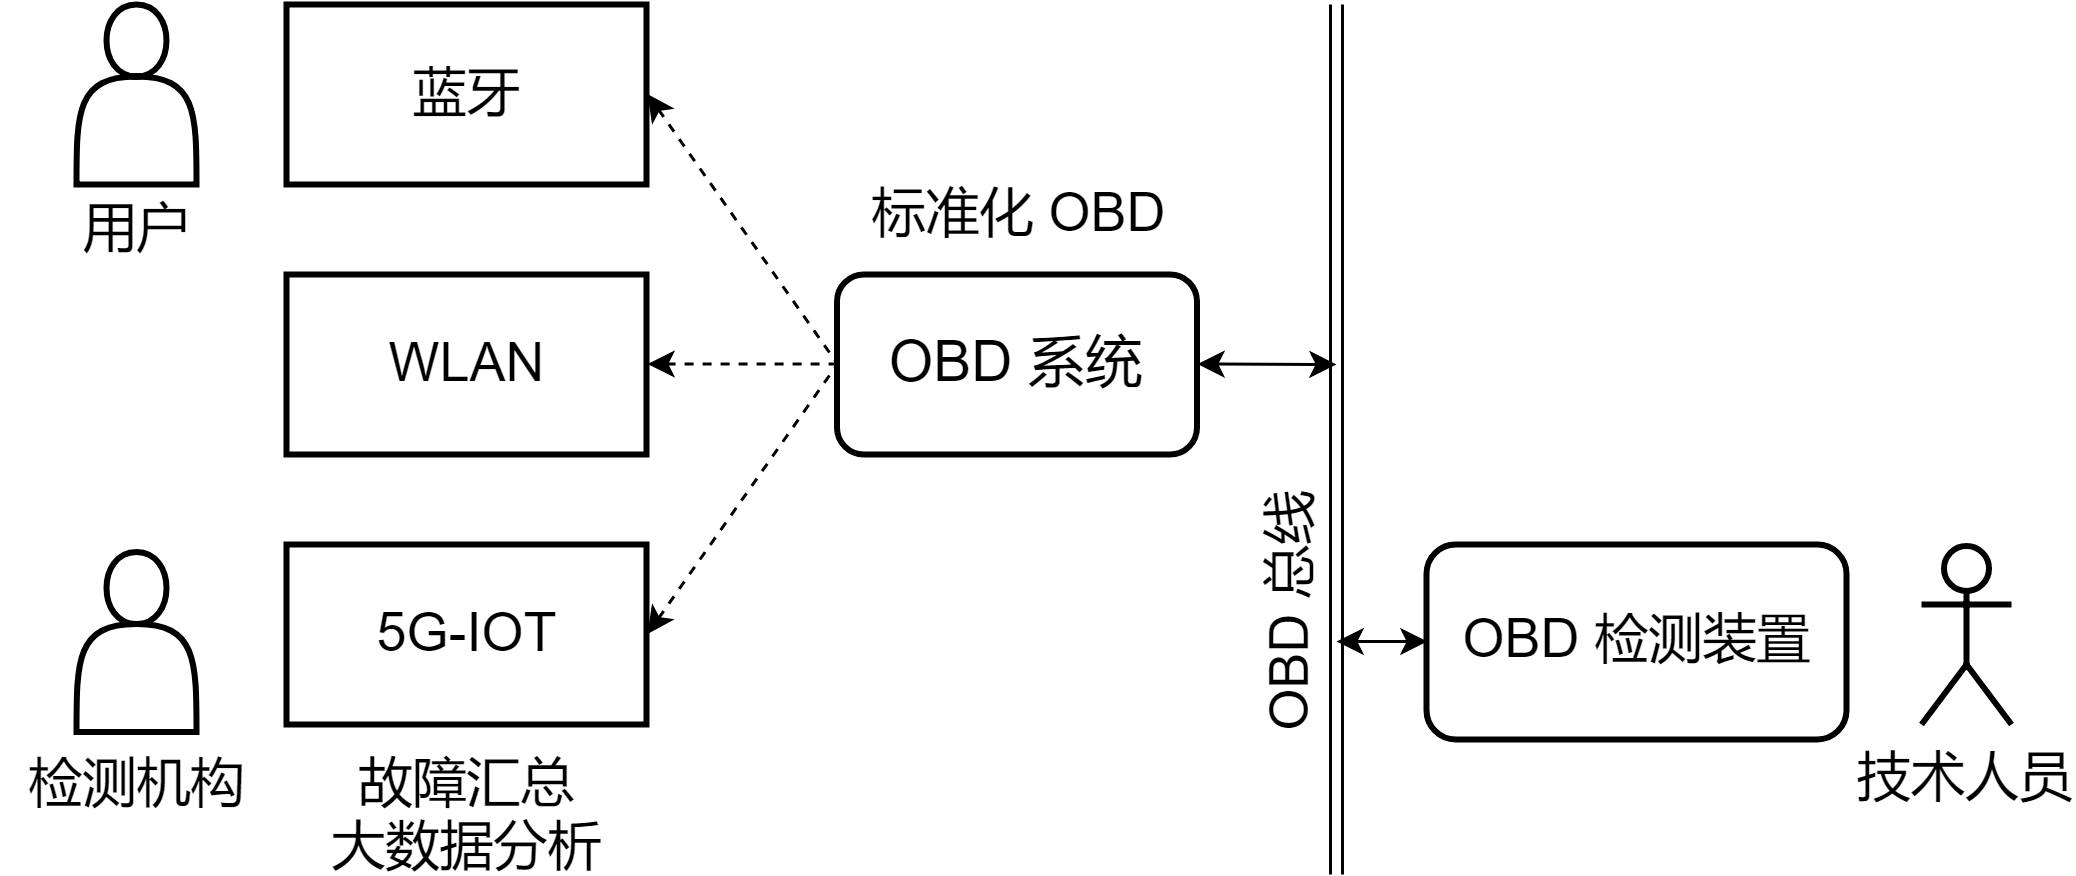
\includegraphics[width=0.7\textwidth]{figures/OBD_future.png}
	\caption{OBD 系统在未来的发展}\label{fig:OBD_future}
\end{figure}

由于电动车技术发展时间较短,故相对于已经在燃油车上使用多年的 OBD 系统来说,电动车的 OBD 系统目前还不太成熟,相关的 ISO 以及 SAE 标准较少。目前已经实施的 OBD 标准,是针对燃油车的排放系统所设置的,对于新的能源系统尚未作出故障的诊断规定。而对于电动车来说,与电动车排放相关的部件即为电池系统和电机系统,所以在传统燃油车上被用作诊断排放相关的 OBD 系统,在目前的电动车上同样应该普及,被用作电池系统和电动机系统的诊断 \cite{Yang2013Research}。

\section{电池箱的 OBD 系统}

电池箱的 OBD 系统是和电池箱的 BMS(Battery Management System 电池管理系统)相协同的。在电池箱内,应该诊断的项目有很多,例如电池箱的箱内温度、压力,开路电压范围,电池的内阻大小,电池的 SOC 范围,电流的大小等等,在诊断之前,OBD 系统需要借助传感器获取这些数据,而 BMS 系统可以通过数据总线提供这些数据,故两个部件必须相互连接;而对于集成 OBD 系统来说,可以在 BMS 系统中设计相应的功能,配合外围的硬件即可实现集成式 OBD 功能。

在目前,电池箱的诊断过程仅仅使用了厂家自行定义的 UDS(Unified Diagnostic Services 统一诊断服务)服务,不同品牌的汽车采用不同的服务码,导致了诊断时不同厂家的车辆产生故障码混乱,而电池箱系统类似于传统油车的发动机,为车辆提供动力,电池箱的故障会引起车辆的能量损耗,故在最新的标准中,为了统一电动汽车诊断流程的规范化,电池箱也被纳入了 OBD 系统的管理范围,在最新的《轻型汽车污染物排放限值及测量方法(中国第六阶段)》(GB 18352.6-2016) \cite{ 轻型汽车污染物排放限值及测量方法(中国第六阶段)} 中的 J.4.14.2.3 部分明确规定了在混合动力汽车中,REESS(电量储存系统)被作为故障检测项目之一,被纳入 OBD 系统必须监测的内容。并且 J.4.14.3 中详细规定了对于电池系统的检测的条件和要求。

综上,可以看到,与其他的诊断协议相比,OBD 诊断系统在协议的规范性、功能性上具有很多优势,在汽车上的应用范围会越来越广,而不仅仅局限于现有的燃油车上。在不久的未来,混合动力汽车将会装配有该系统,而且,可以预测纯电动汽车也会逐渐使用 OBD 系统,OBD 技术将会成为汽车诊断领域的核心技术。

\subsection{物理接口}

在 OBD 相关协议中定义了 OBD 总线使用的物理接口,该接口的形状如图 \ref{fig:OBD_plug} 所示。在 SAE J1962 中规定了该接口的引脚排布,接口的形状为双排 8 Pin 插座,插座的形状有两种类型,被分为 A 型(左)和 B 型(右),不同类型 OBD 接口的引脚的定义相同,并直接接受汽车电池系统供电  \cite{杨沛2017基于OBD接口的低压保护电路}。在此之外,该标准中规定了 OBD 接口必须在转向盘两英尺的范围之内,不得离驾驶员过远。

\begin{figure}
	\centering
	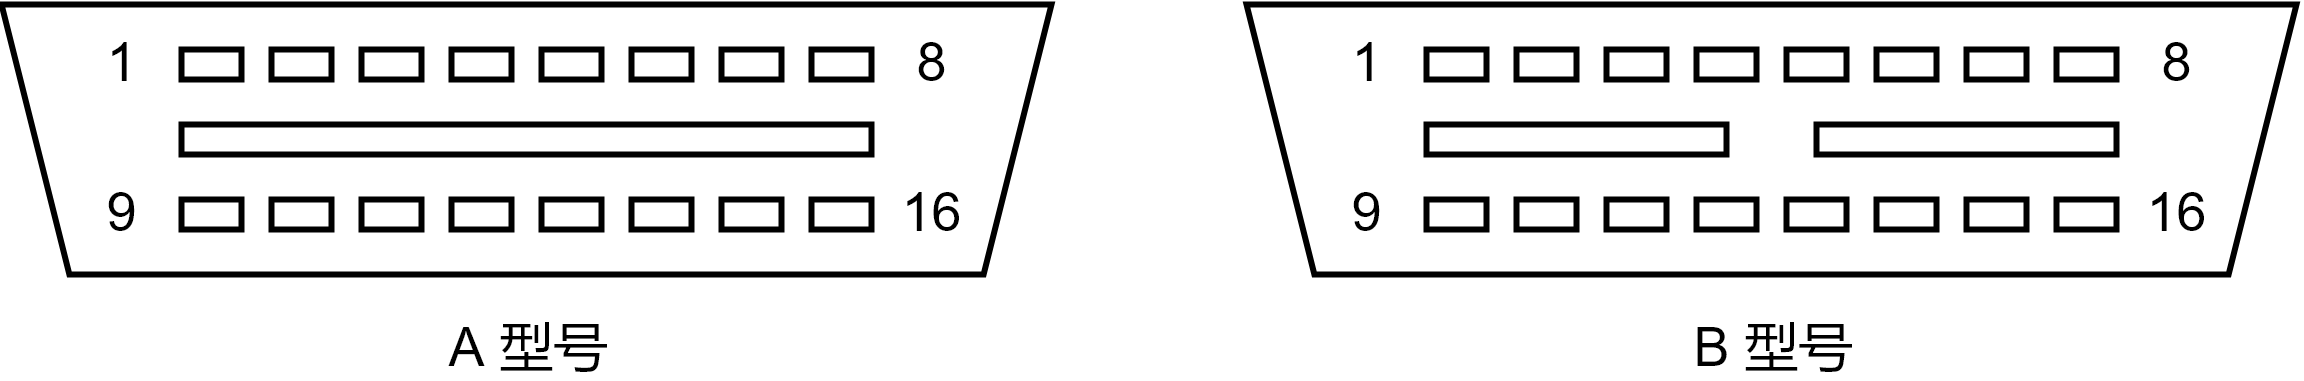
\includegraphics[width=0.7\textwidth]{figures/OBD_plug.png}
	\caption{标准化 OBD 接口}\label{fig:OBD_plug}
\end{figure}

该插座的不同编号的引脚代表了不同的类型,引脚的分布图如表:

\begin{table}
	\centering
	\caption{OBD 引脚定义图} \label{tab:OBD_plug}
	\begin{tabular*}{0.8\textwidth}{@{\extracolsep{\fill}}cc}
		\toprule
		编号			&定义		 \\
		\midrule
		2, 10           & SAE J1850(PWM/VWM)协议总线    \\
		4, 5            & GND(针对所有的协议总线)  \\
        7, 15           & ISO 9141-2/14230-4(KWP2000)协议总线 \\
        6, 14           & ISO 15765-4 (CAN) 协议总线 \\
        16              & 12V Vcc      \\
        其他            & 保留         \\
		\bottomrule
	\end{tabular*}
\end{table}

\subsection{OBD 通信协议电气标准}
在 OBD 系统中,并没有指定特定某一种的协议物理以及链路层的类型,在 OBD 的协议中,可以使用的底层物理和链路层的协议目前可以选择有 3 种,分别为 ISO 9141,也就是目前在旧式汽车上使用的 KWP2000 总线,俗称为 K 线;SAE J1850 中规定的 PWM 和 VPM 协议,又被称之为脉冲宽度调制(Pulse Width Modulation)协议和可变脉冲宽度调制协议(Variable Pulse Width Modulation);ISO 15765-4,基于 CAN 总线的 OBD 协议 \cite{Li2013Design}。

\subsubsection{KWP2000 协议}
在 ISO 9141 中规定了一种被称之为关键字协议 2000 (Keyword Protocol 2000)的标准,它又在 ISO 14230 中被详细规定了物理层和链路层的标准。KWP2000 协议又被称为 K 线通信协议,它是利用一根双向的数据传输线(K-line)。在 K 线(K-line)上,数据以半双工的模式进行通信,其网络结构如图 \ref{fig:OBD_K-line} 所示,在 K 线通信中,可以选择性的增加一根 L 线(L-line),L 线起到唤醒作用。KWP 2000 传输中,将低电平,也就是总线电压小于 $ 20\% Vbus$ 视作逻辑 0;将高电平,也即是总线电压大于 $ 80\% Vbus$ 视作逻辑 1。KWP2000 协议的数据传输速度较慢,其波特率范围为 1.2~10.4 kbps,一次传输可以传输最多 255 字节。由于速度过慢,在 2008 年后,该类型总线不再使用在 OBD 系统上。

\begin{figure}
	\centering
	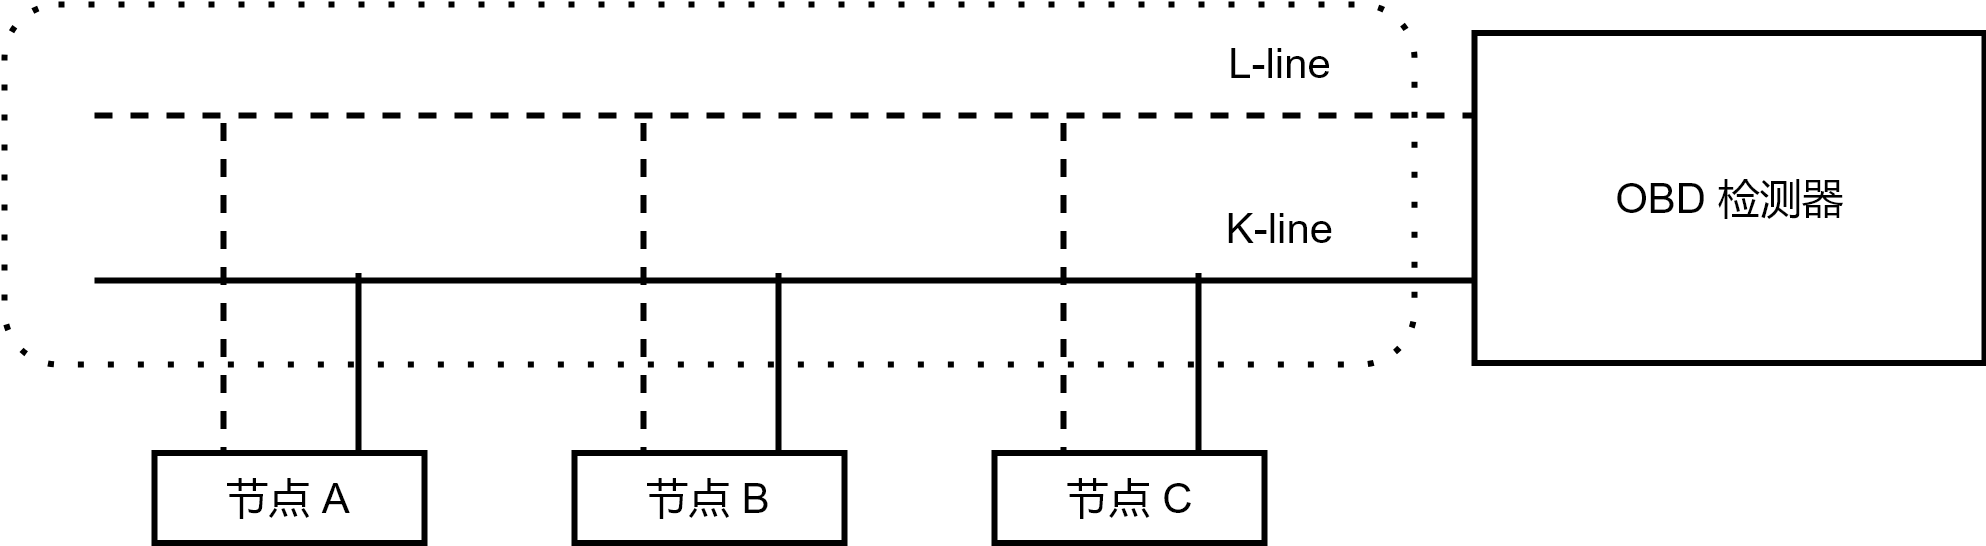
\includegraphics[width=0.7\textwidth]{figures/K-line.png}
	\caption{KWP2000 总线示意图}\label{fig:OBD_K-line}
\end{figure}

\subsubsection{PWM 和 VPM 协议}
PWM 和 VPM 协议是一种应用于 OBD 诊断服务中的总线协议,其标准在 SAE J1850 中被规定,其中使用较多的是基于 PWM 的 OBD 协议。该协议基于脉冲宽度调制原理,利用信号线上每个周期不同的占空比来判断逻辑值。由于 PWM 和 VPM 也是采用单线半双工通信的模式进行通信,通信时速度较慢,PWM 传输速率被固定设定为 41.6 kbps,VPM 传输速率被设定为 10.4 kbps。由于该总线的速度同样较慢,在目前最新生产的车型上,该类型总线已经被淘汰。

\subsubsection{CAN 协议}
CAN 协议作为以上两种协议的替代者,拥有高速,高可靠性的特点。CAN 总线的结构如图 \ref{fig:CAN} 所示,CAN 总线的末端有两个终端电阻,在 ISO 11898-2 中规定了在 高速 CAN 总线上终端电阻的阻值为 120 欧姆。CAN 总线为两线制总线,两根信号线分别被称为 CAN\_High,CAN\_Low。在 CAN 总线上,逻辑值电平有两种,一种被称之为隐性电平,另一种被称为显性电平。隐性电平时,两根线中所有的节点均不驱动信号线,信号线间因为存在终端电阻,故不存在电势差,但是总线的电压值在 2.5V 附近,此时节点检测到无信号,便会认定总线处于空闲状态,或者在传输的过程中,认定总线上的逻辑值为 1;显性电平时,总线上某一节点或多节点将 CAN\_High 信号线驱动向 5V,而将 CAN\_Low 驱动向 0V,在这种情况下,总线上所有的节点都会检测到总线上处于被占有状态,或者在传输数据时,认定总线上的逻辑值为 0。CAN 总线采用两线半双工传输的优势是,信号的判断依靠两根线的共同状态,在传输信号的时候,两根线可以起到差分信号的作用,若总线上发生了电气故障,两根线总线可以快速发现总线故障,提高了传输数据的可靠性。

\begin{figure}
	\centering
	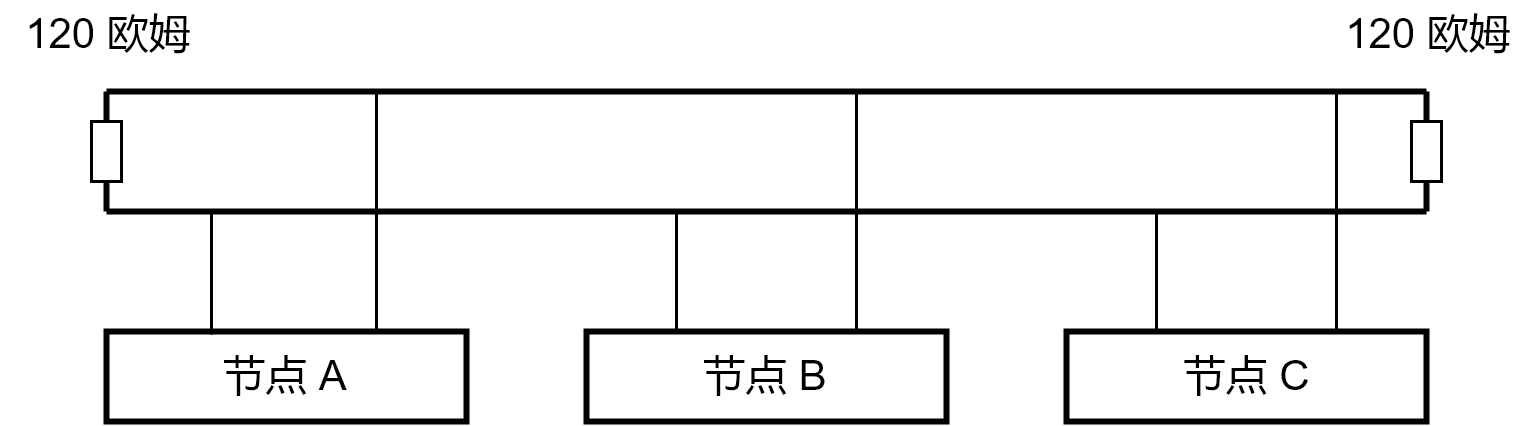
\includegraphics[width=0.7\textwidth]{figures/CAN.png}
	\caption{CAN 总线结构示意图}\label{fig:CAN}
\end{figure}

由于 CAN 总线采用了差分信号机制,与此之外,在数据链路层,CAN 总线提供了一个包含 CRC 校验的信息发送机制,所以 CAN 总线上传输的数据具有相当的可靠性,可以有效抵抗电磁干扰所带来的错误。在发送的时候,传统的总线协议在高速情况下的数据干扰因素在 CAN 总线上被校验机制减弱,故 CAN 总线可以达到更高的传输速率,在 ISO 11898 中规定的高速 CAN 总线信息传输速率最快可以达到 1 mbps。由于 CAN 总线具有优越的性能,故已经被广泛的应用到汽车通信领域,目前几乎所有的车辆都搭载有 CAN 总线。针对此,本文所设计的 OBD 系统是基于 CAN 总线协议的,在物理层和数据链路层使用了标准的 CAN 协议。

\section{OBD 系统设计}
本文所设计的 OBD 系统是符合现行标准的硬件系统,故其通信协议应遵守在 ISO 标准中所定义的 OSI 7 层网络模型结构,如表 \ref{tab:OBD_OSI} 所示。除此之外,在功能上应该具备一套完备的 OBD 系统所应具备的所有功能,包括故障码的储存,MIL 灯的点亮,和响应外置 OBD 诊断仪所提出的 OBD 服务请求功能。

\begin{table}
	\centering
	\caption{OBD OSI 网络结构} \label{tab:OBD_OSI}
	\begin{tabular*}{0.8\textwidth}{@{\extracolsep{\fill}}cc}
		\toprule
		OSI 层			&标准		 \\
		\midrule
		应用层           & ISO 15031-5 / SAE J1979    \\
		展示层           & SAE J2012 DA / SAE J1979 DA \\
        会话层           & ISO 14229-2 \\
        传输层 / 网络层           & ISO 15765-2 \\
        链路层 / 物理层           & ISO 11898      \\
		\bottomrule
	\end{tabular*}
\end{table}

\subsection{硬件配置}
为了满足 OBD 系统的需求,首先需要选择合适的微处理器芯片,同时选择外围的电路需要哪些电子元件。为了实现 OBD 系统中最关键的故障码存储的功能,必须在外围使用一个额外的 NVRAM(非易失性随机访问存储器)来进行故障码的存储,OBD 标准中并未指出应该使用哪一种特定类型的存储器,而为了达成非易失性存储,可以选择的存储器方案有:单独供电的 SRAM 存储区或 DRAM 存储器,EEPROM,或者是使用 Flash 闪存进行存储 \cite{Matas1997Memory}。

\begin{itemize}
	\item 使用单独供电的 SRAM 或 DRAM 存储器,在硬件设计中,应当将微控制器的供电线路和存储器的供电线路分割,使用纽扣电池或者干电池单独对于存储器供电,该方案的优点是,使用该方案的两种 RAM 存储器在存储速度上优于另外两种,数据读写速度在 10 纳秒到 100 纳秒之间。除此优点之外,该方案的存储器读写寿命极长,读取和写入的时候不存在物理损耗现象,故适用于频繁高速大容量读写的应用场所。缺点是该方案的供电线路设计较为复杂,数据的保存需要供电系统进行间隔刷新供电,而且该类型存储器元件价格较高,会提高设计的成本。
	\item 使用 EEPROM 存储器进行数据的存储,EEPROM 又被称作带电可擦可编程只读存储器。该方案的优点为,存储器在断电之后可以保存系统内的数据,并不需要单独的供电,而且成本较低,寿命方面较长,可以达到百万次的写入擦除次数,缺点是容量较小,在市面上可以使用的最大的 EEPROM 容量在 2 MBits 左右,而且读写速度很慢,由于写入时需要一次性写入整个扇区,所以平均的写入时间在数毫秒左右,在高速度的读写应用条件下并不能达到使用要求。
	\item 使用 Flash 存储器,Flash 存储器又被称作闪存,是一种类似于 EEPROM 的非易失性储存器件。Flash 具备 EEPROM 所具备的所有优点,并且与 EEPROM 相比,Flash 储存的单位容量的数据成本更低,写入的速度更快,每次写入一页数据仅仅只有几十微秒,而且 Flash 储存器的价格相当低廉,被广泛的使用于需要储存的各个领域,包括 U 盘,固态硬盘都采用了 Flash 存储器作为存储的介质。但 Flash 存储器的缺点是 Flash 的擦除次数有限,目前常见的 Flash 存储器的擦除次数都在十万次以下。
\end{itemize}

最终本文选择使用 Flash 存储器作为 OBD 系统中的储存器件,因为在 OBD 使用的过程中,数据量较小,但是由于 OBD 系统需要监视实时的数据,数据周期一般只有几十毫秒或者几百毫秒,需要快速的写入和读取,故 EEPROM 并不符合 OBD 的使用需求,而若使用 SRAM 或 DRAM 则会大大增加成本,且需要设计外围的供电电路,使用电池供电,增加了供电所需的成本,而 Flash 价格低廉,而且容量较大,速度也符合 OBD 的应用场景。

\subsection{电路原理图}
电路原理图的完整设计图纸,见附录 A 图 \ref{fig:sheet}。

为了满足调试的需求,在外围使用了来自 FTDI 公司生产的 FT232H 型号芯片,该型号芯片可以通过 USB 接口连接计算机,并且可以同时通过引脚直接访问存储器件,在脱机状态下可以读取 OBD 系统中存储的数据,方便了调试的过程。

\subsubsection{供电电路}
供电电路的设计主要是针对电路板上的各芯片的供电部分进行设计,该电路板的供电方式是使用板载的 USB 接口进行供电,由于 USB 接口的热插拔特性,在插入和拔出的瞬间在线路上会产生较大电流,也会由于静电作用在外壳和电路间产生巨大电压,故在 USB 接口中将数据线 DM DP 用两个 PGB10106603 TVS 瞬态抑制管接地,并且在数据线上使用 0 欧电阻 $R_2$ 和 $R_4$ 作为电路的安全防护作用。USB 接口的 $V_{BUS}$ 引脚为供电电源,其电平为 $5V$,为了抑制该电源线上的高频噪声,在这里使用了规格为 $600R \quad 0.5A$ 的磁珠 $FB_1$,供电电路的设计如图 \ref{fig:USB-SCH} 所示。

\begin{figure}
	\centering
	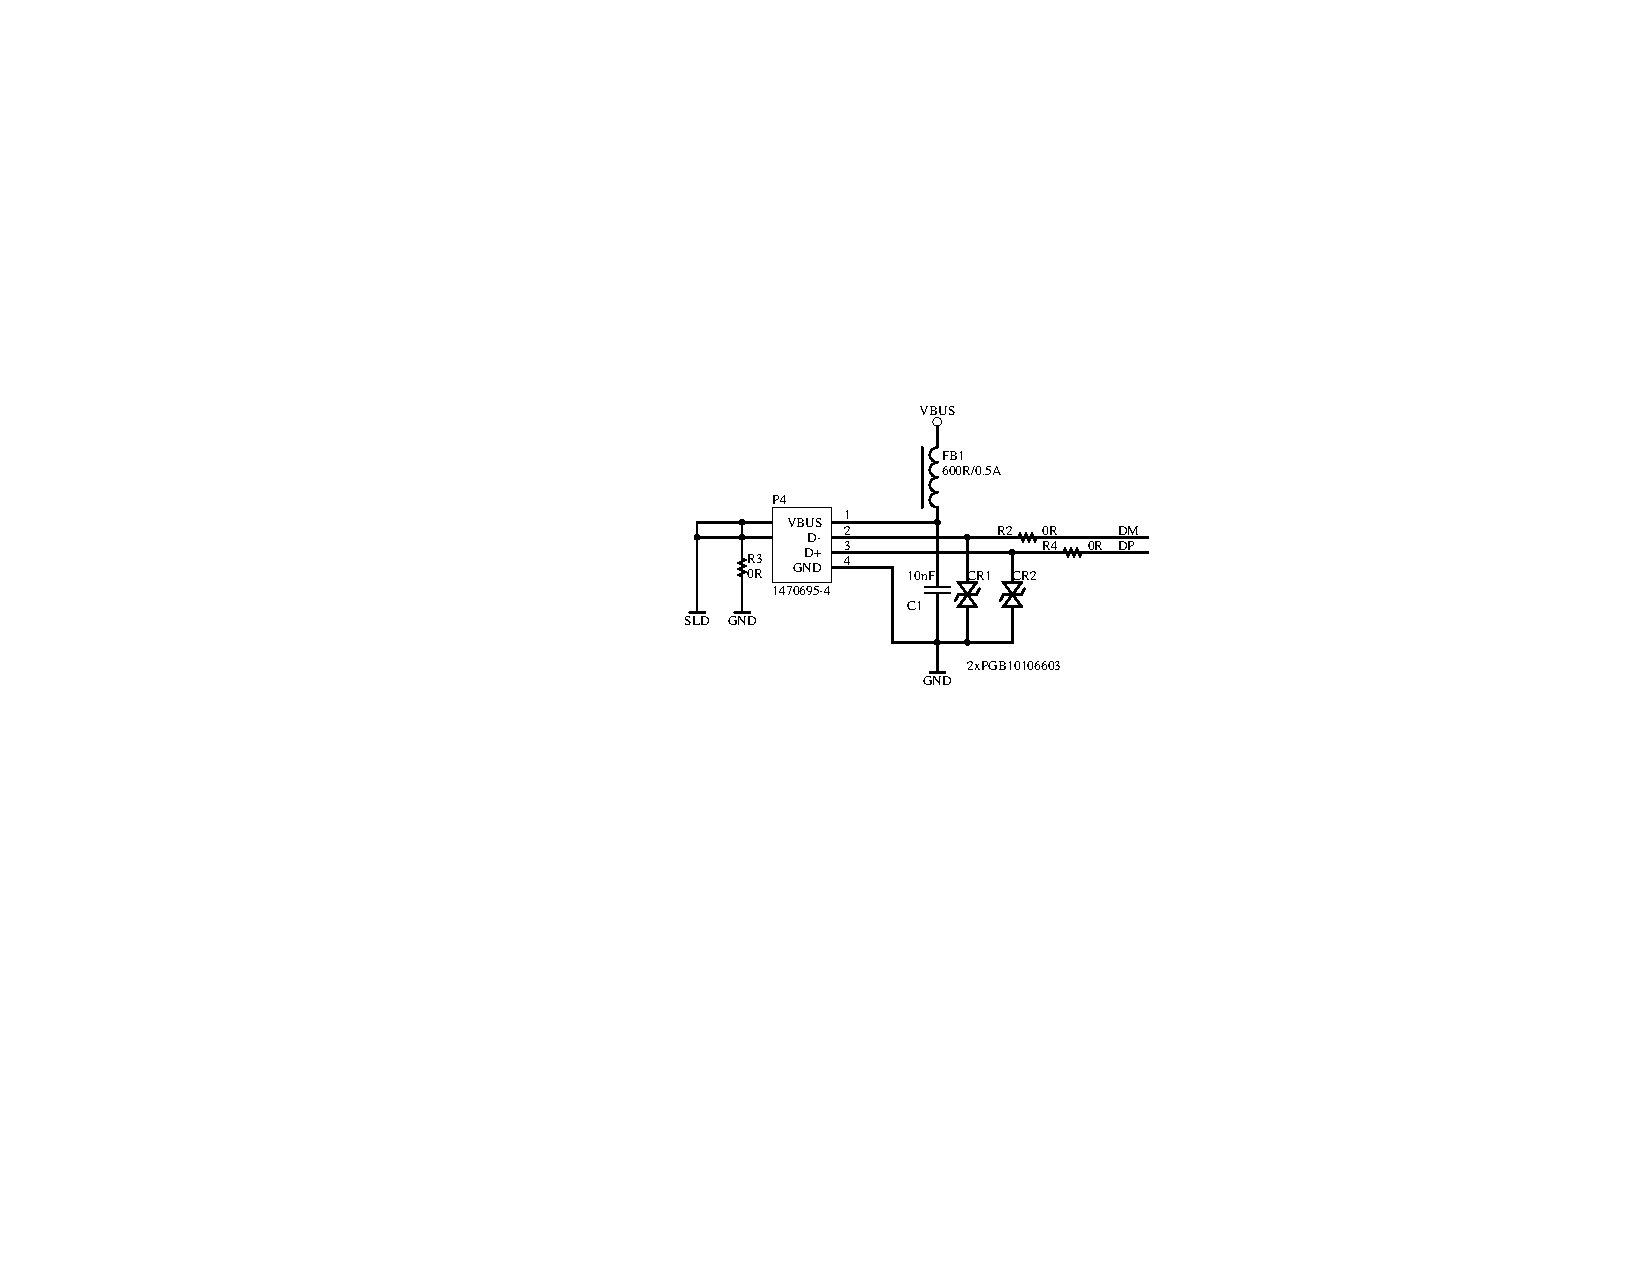
\includegraphics[width=0.5\textwidth]{figures/USB-SCH.pdf}
	\caption{OBD 系统电路供电原理图}\label{fig:USB-SCH}
\end{figure}

在芯片与外围的元器件的滤波电容的设计如图 \ref{fig:filtering-SCH} 所示,其中芯片的 $5V$ 供电电压被内部的 LDO 降压器降压为 $3.3V$ 和 $1.8V$ 供电给芯片自身,故在滤波设计中需要将三种电压分别设置电容滤波网络。

\begin{figure}
	\centering
	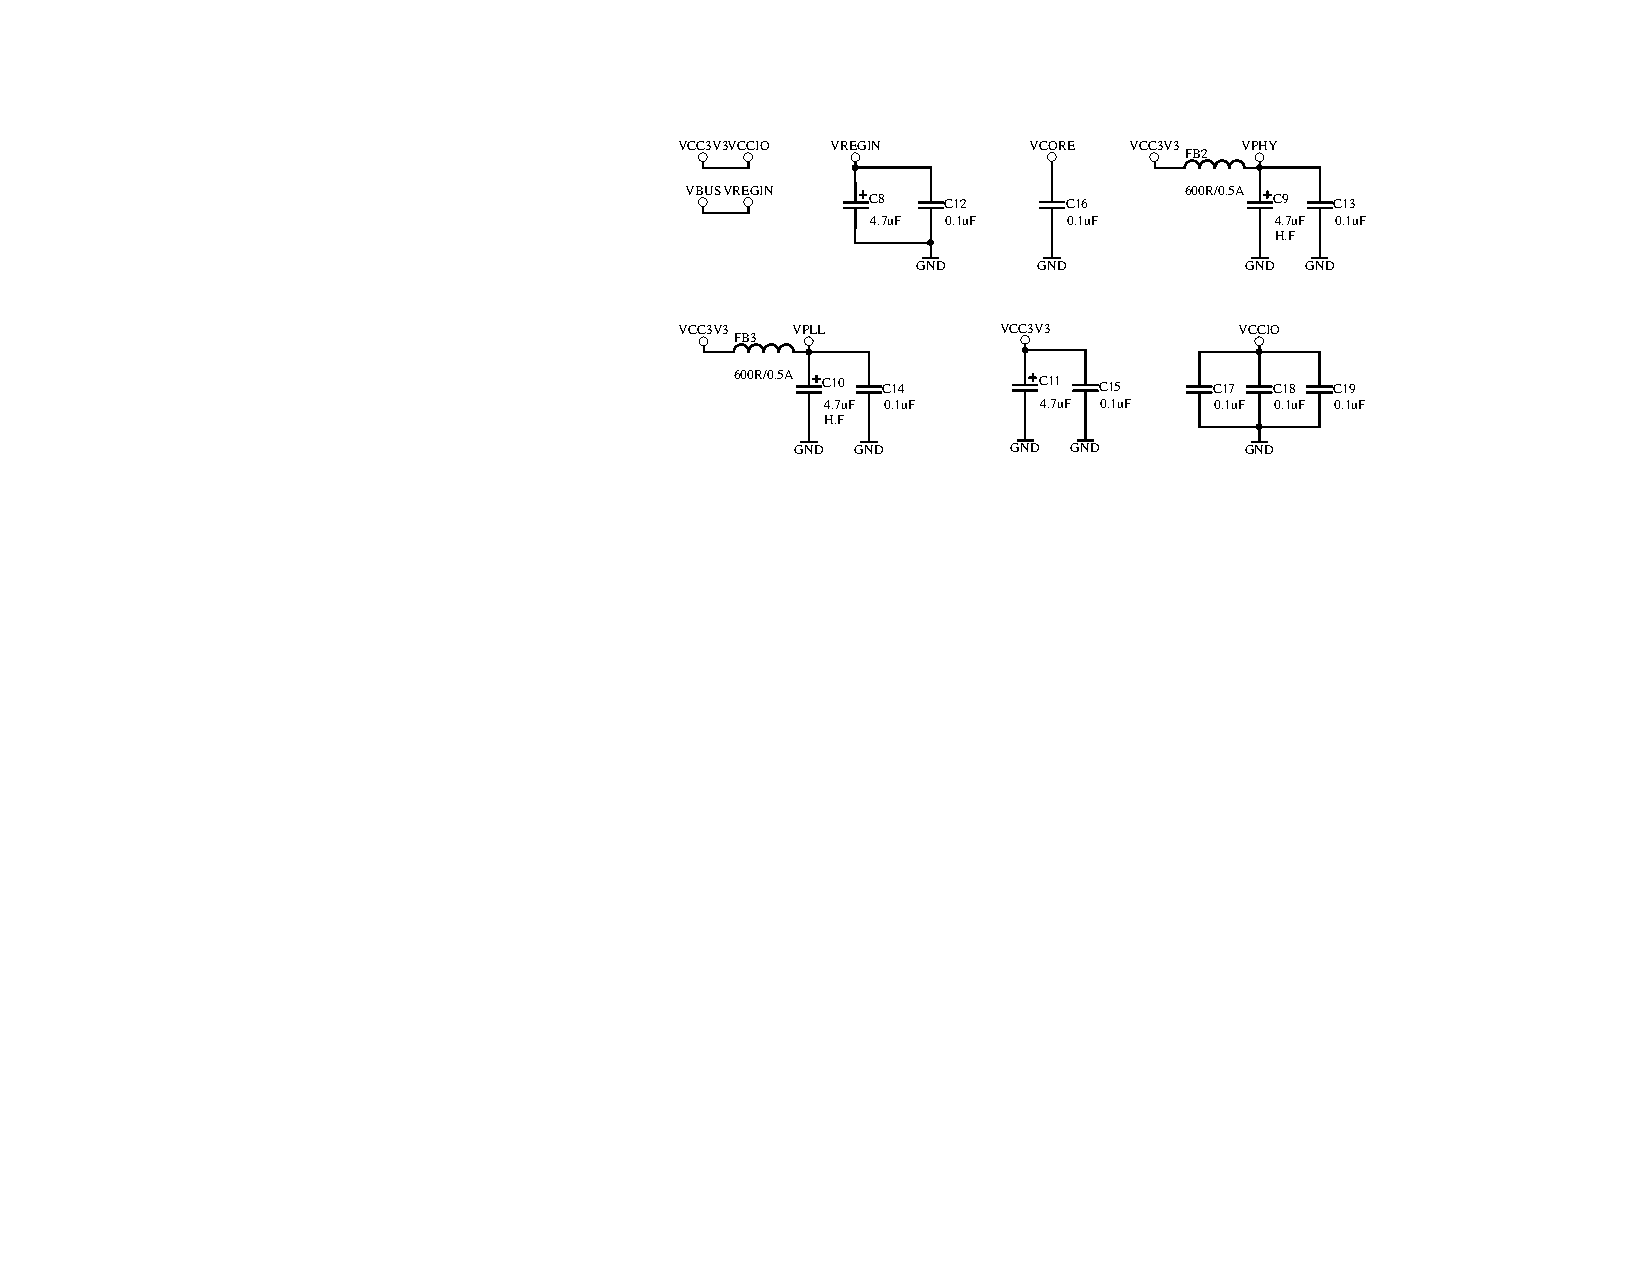
\includegraphics[width=0.5\textwidth]{figures/filtering-SCH.pdf}
	\caption{OBD 系统滤波网络原理图}\label{fig:filtering-SCH}
\end{figure}

\subsubsection{晶振电路}

在电路中晶振使用了 12MHz 的无源晶振,匹配的电容为 $20pF$,电路的设计如图 \ref{fig:XCSIO-SCH}。

\begin{figure}
	\centering
	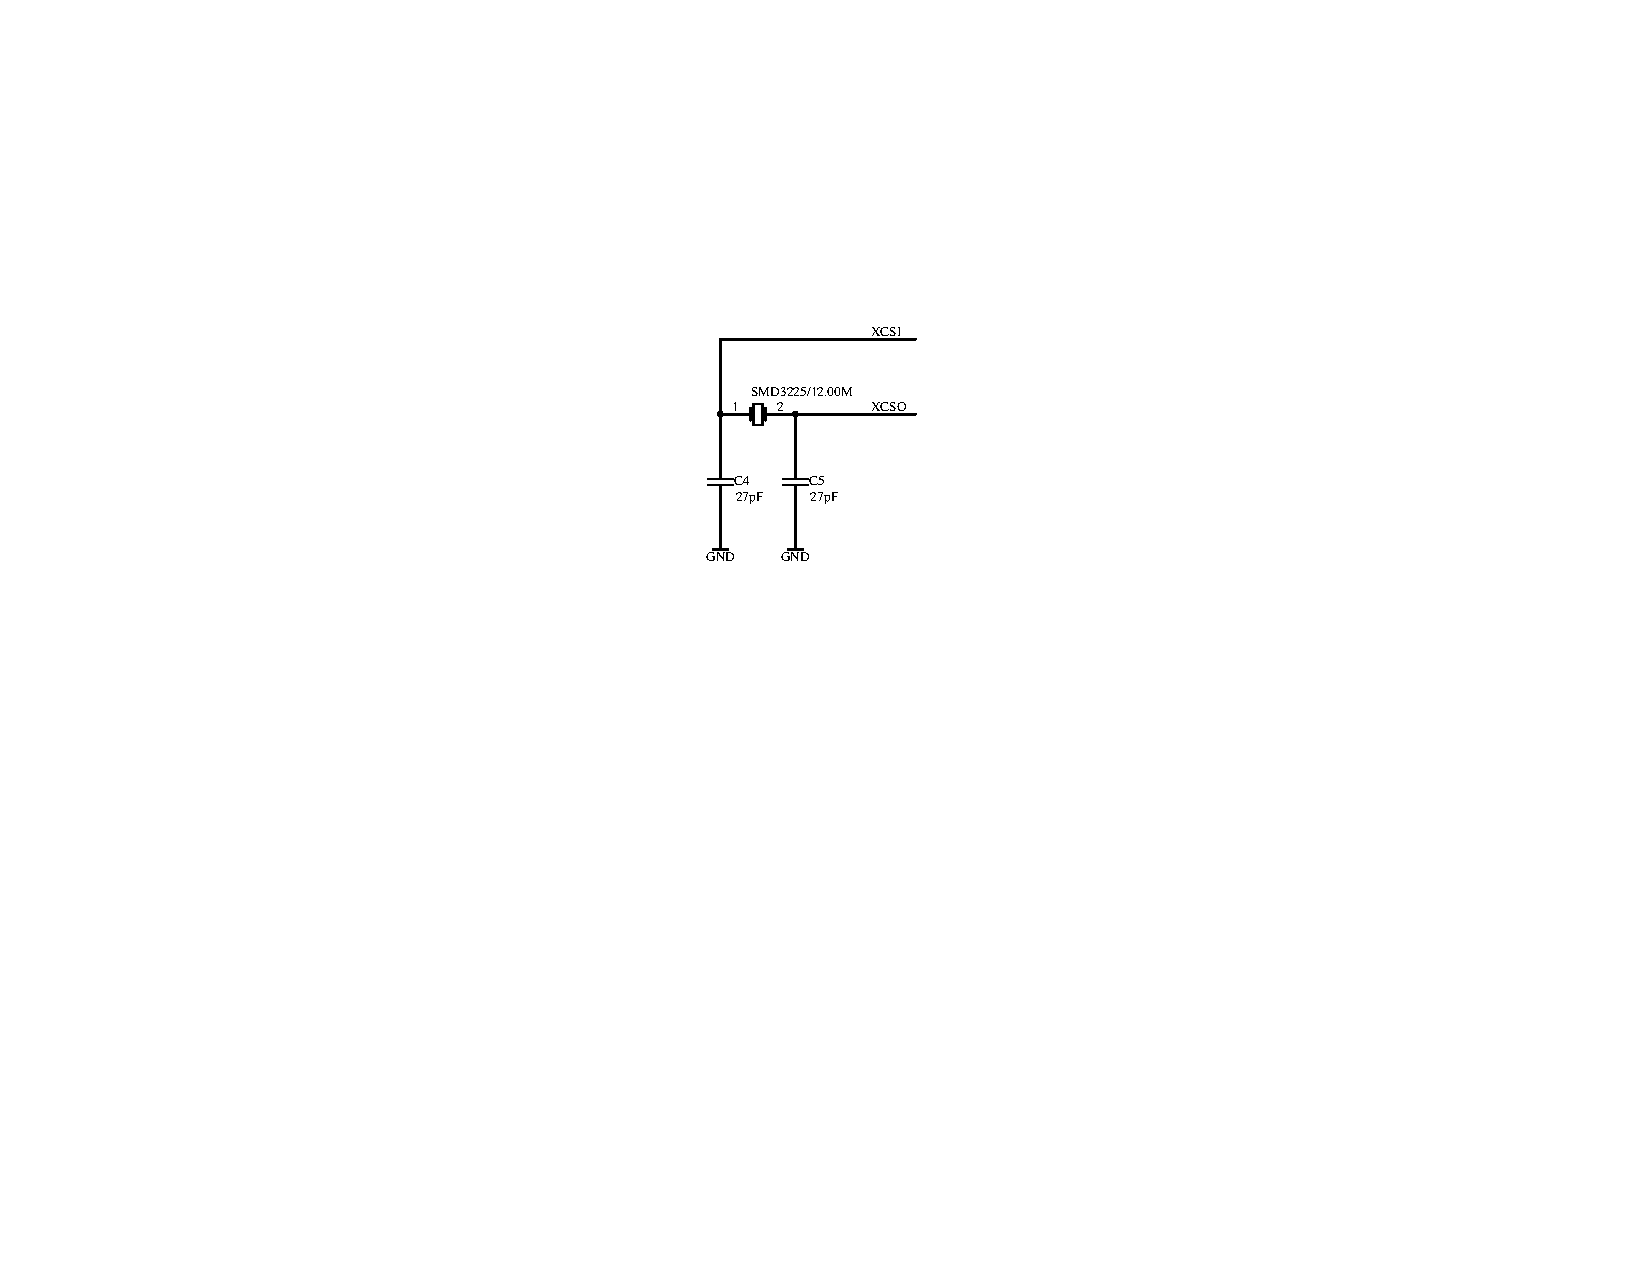
\includegraphics[width=0.5\textwidth]{figures/XCSIO-SCH.pdf}
	\caption{OBD 系统晶振电路原理图}\label{fig:XCSIO-SCH}
\end{figure}

\subsubsection{储存电路}
储存的元器件有两种,一种是被用于存放电路板设置内容的 EEPROM 存储器,另外一种是存放 OBD 故障信息的 Flash 储存器,储存器的电路如图 \ref{fig:EEPROM-SCH} 所示。

\begin{figure}
	\centering
	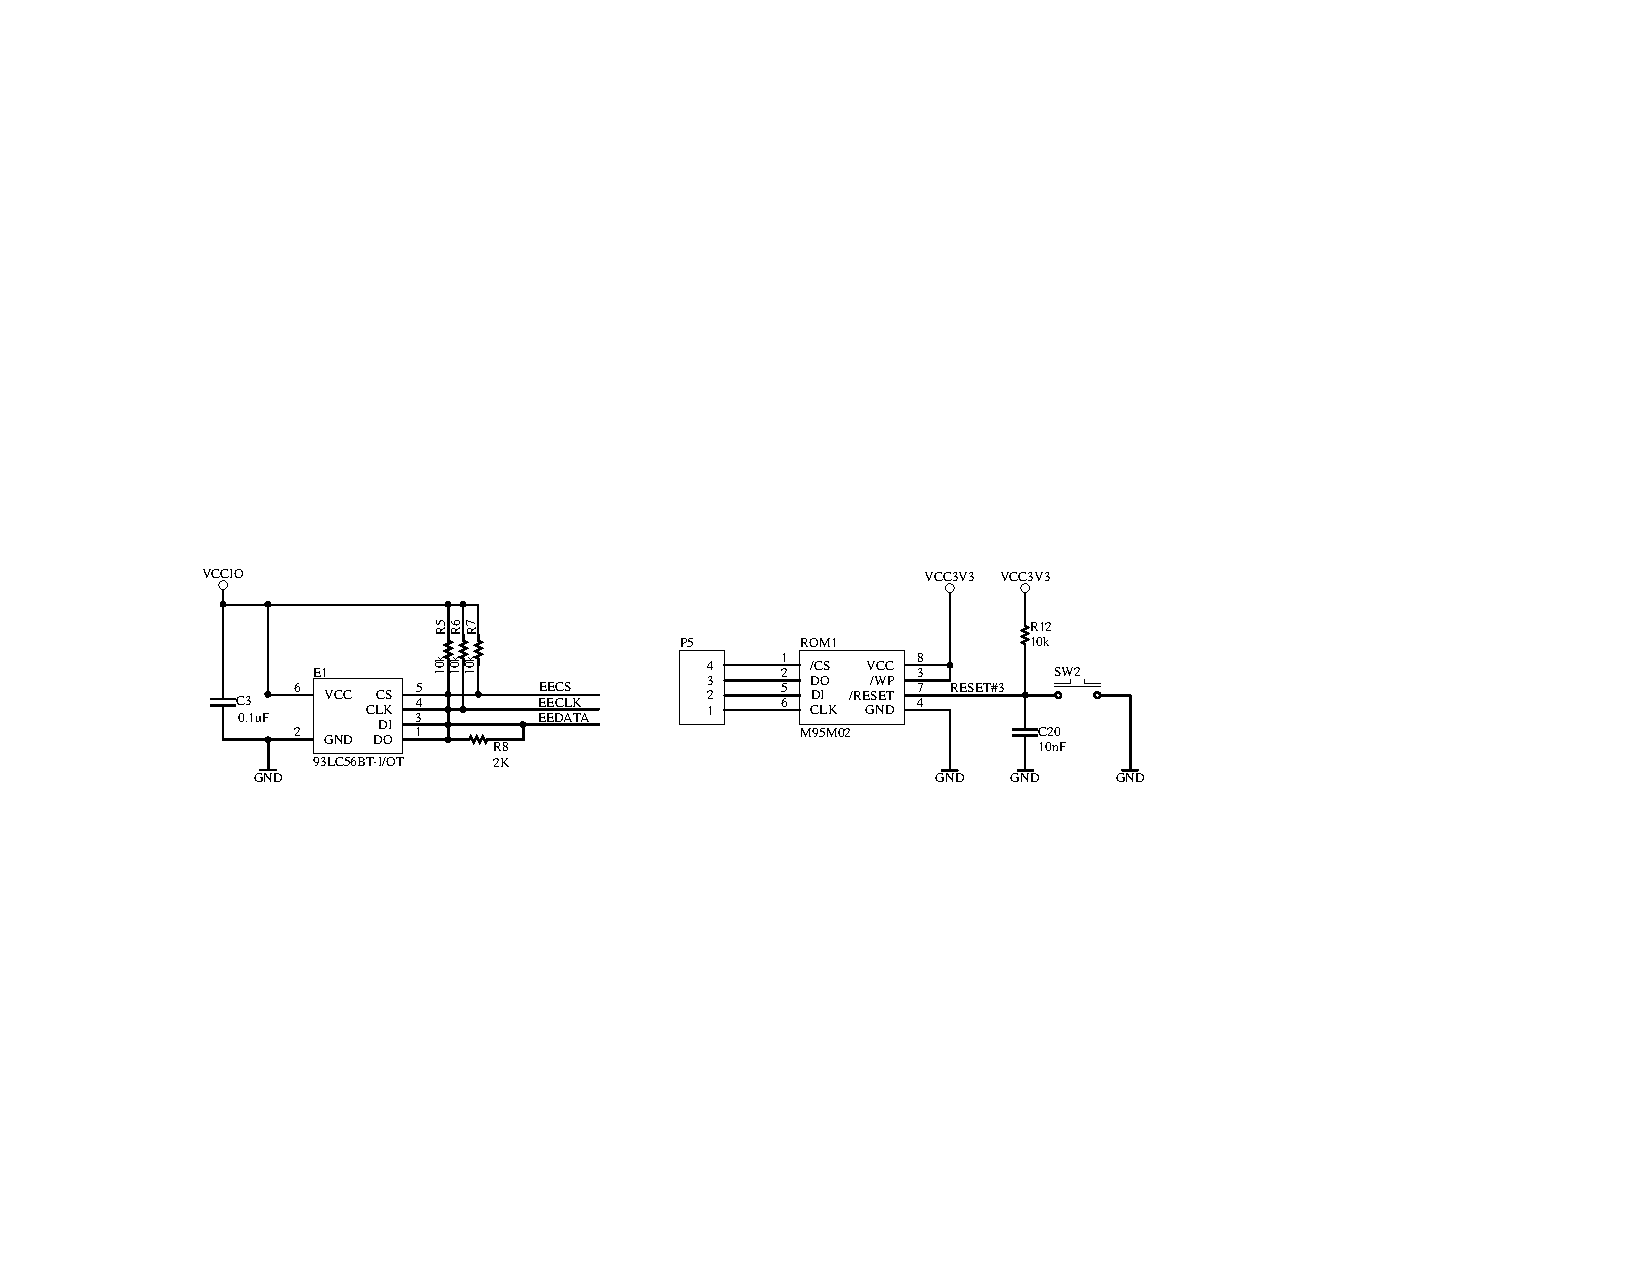
\includegraphics[width=0.35\textwidth]{figures/EEPROM-SCH.pdf}
	\caption{OBD 系统储存原理图}\label{fig:EEPROM-SCH}
\end{figure}

\subsubsection{PCB 电路图}
该 OBD 系统的 PCB 电路图的设计如附录 B 图 \ref{fig:PCB} 所示。该 PCB 电路板已经加工完成,完成了焊接以及调试的过程。

\subsection{OBD 协议栈的开发}
在硬件方面实现了相关功能的元器件的连接之后,在软件层面本文将对于 OBD 协议栈中的设计流程进行简略的介绍。由表 \ref{tab:OBD_OSI} 可以看到首先在在设计 OBD 的软件设计前,需要首先了解 OBD 的网络结构与消息机制。OBD 的网络结构可以分为三个主要的部分,物理层与链路层、网络层与传输层、展示层与应用层,层与层之间的消息传递使用到了 PDU(Protocol Data Unit)协议数据单元为消息的载体。在消息机制方面应该采用消息队列机制,在网络层每部分面设计缓冲数据块,这样系统在高负荷状态下同样可以利用缓冲保证系统稳定性,确保所有的 OBD 服务均能够得到处理,同样提高了系统效率。

\subsubsection{OBD 物理层与链路层}
在 OBD 协议栈中物理层和链路层属于与硬件相关的协议底层 \cite{Zheng2008A},该层协议的实现基于硬件,在 CAN 总线上有 CAN 控制器和 CAN 收发器,其中 CAN 控制器负责数据链路层协议,CAN 收发器负责物理层协议,在市面上常用的单片机中一般集成了 CAN 控制器,可以通过对于单片机中的寄存器的数据控制,通过内置的移位寄存器,达到 CAN 总线的数据发送和接收。

\subsection{OBD 网络层与传输层}
OBD 网络层与传输层主要负责的任务是有关数据传输过程中的以下多个内容:

\begin{itemize}
	\item 数据的多帧分割与重组。
	\item 多帧发送的顺序与流程控制。
	\item 网络参数的设置。
\end{itemize}

众所周知,标注的 CAN2.0A 标准中规定了 CAN 数据帧的数据域长度为 0$\sim$8 个字节,若想要一次性传输多字节,则必须将数据分多帧传输。在 OBD 的网络层与传输层协议中,实现了最长的 4095 个字节的传输。数据在网络层之上的协议层则被抽象成为数据包的格式,不需要考虑数据的传输问题。

多帧传输的过程中,传输的过程较长,在总线上将会进行接收方和发送方的沟通,每隔若干个发送 CAN 帧之后,发送方将会等待接收方发送一个状态指示帧决定接下来的发送数据长度。

网络参数主要是在 OBD 协议网络上的地址参数,如何定义 OBD 节点的地址;OBD 网络的时间参数,发送方应该在一定的时间内响应 OBD 服务以及发起数据传输,而接收方应该设置超时参数,一旦发送方在超时时间内未作出有效的响应,则接收方应该重新发起 OBD 请求。

\subsection{OBD 展示层与应用层}
 OBD 展示层和应用层是面向于用户的内容,该层的开发是 OBD 系统的关键,它决定了 OBD 系统提供给用户的数据,如果将 OBD 系统抽象为网络上的服务器,则用户为客户端,当客户端发起了车辆的诊断请求之后,OBD 系统应该对于该请求作出回应,而应答的内容收到展示层和应用层的标准规定。

OBD 展示层内容主要是车辆故障码的定义以及车辆的诊断过程中如何认定故障的流程,该层的内容需要参考现有的标准包括 SAE J2012 和 ISO 15031-6。OBD 协议应用层的标准包括 SAE J1979 和 ISO 15031-5。在实现的过程中应该遵守标准,这样才能实现报文的通用,不遵守标准会导致系统失去通用性,失去了 OBD 系统的意义。

%%==================================================
%% conclusion.tex for BIT Master Thesis
%% modified by Liu xiahua
%% version: 0.1
%% last update: May 25th, 2018
%%==================================================


\begin{conclusion}

电能动力系统中的主要组件是电动机和发电机、电池或能量存储系统以及功率电子驱动系统。但是相比于其他的电动车技术,电池技术是阻碍纯电动汽车在大众市场上发展的主要技术之一。本文对于现有的电动汽车领域的技术进行了回顾和总结,对于我国的电动汽车发展的现况和国外进行了对比,在电动汽车领域,目前我国汽车工业的技术与国外的汽车企业相比存在一定的差距。

在电池箱设计技术中,最首先要进行研究的,也是最有商业意义的就是电池箱参数的匹配,因为市面上的大多数混合动力车辆还是基于原有车辆的动力系统开发的,参数匹配在实际生产中有重要意义。本文提出了一种新型的混合动力汽车的电池箱参数匹配的方法,在给定的汽车的行驶动力性指标下,利用车辆的动力学方程,分别通过对于电池箱的功率和能量两部分参数计算,确定电池箱的参数。仿真的结果验证了本文理论计算正确和有效,也同时反映了电池参数匹配中,有许多因素均会影响参数匹配的结果,对于电池参数模型的确定要考虑更多因素。而在电池箱的机械设计方面,现有与电池设计有关的标准大多数出于对电池安全方面考虑。本文分别对于单体、模组、整体和机械连接部分进行了设计,考虑到电池箱的抗振,热管理方面,可以对于现有的设计进行完善和补充。

由于电池箱作为电动汽车的储能元件,是电动汽车中最重要的部件之一。而对于电池箱等电气系统的诊断在过去的十年内是由各个汽车企业自己定制的,不具备行业统一的标准,这也对电动汽车的维修带来了困难。本文中设计的 OBD 系统是基于标准 OBD 协议设计的,提高了诊断流程的统一性,规范故障的条件定义和故障码的定义,该系统的设计具有行业前瞻性意义,响应了我国政府的最新要求。本文在设计过程中对于多种硬件方案进行了分析,在最后进行了相关电路原理图以及 PCB 的设计。

总体来说,本文的设计跨越了电池系统设计的数方面,包含了动力参数、机械模型、电子线路、通信数个系统的设计。虽然设计范围较广,在设计时各因素不能够完全覆盖,但是本文提出的电池参数匹配模型和机械模型以及电子电路的设计,在仿真校验和实际测试中性能优良,具有参考的价值。在最后,本文对于电池匹配参数模型的优化以及热管理系统等后续设计提供了思路和方法,在未来的研究中可以进一步完善和改良。

\end{conclusion}

%% 参考文献,五号字,使用 BibTeX,包含参考文献文件.bib

% 致谢
%%==================================================
%% thanks.tex for BIT Master Thesis
%% modified by yang yating
%% version: 0.1
%% last update: Dec 25th, 2016
%%==================================================

\begin{thanks}

本论文的工作是在导师程夕明老师的指导下进行的,在论文的写作的初期我遇到了许多问题,但在老师的悉心帮助下全部都顺利解决。在进行参数匹配的过程当中,老师对于我的匹配计算过程进行了指导,指出了我在计算过程中的错误,并且提供了匹配中所需要的相关参数,在第四章中对于本文电池箱的诊断系统设计也提出了设计的建议。感谢北京理工大学电动车辆国家工程实验室,韩孟佐师兄不吝抽出时间做实验,为我的论文中的电池匹配章节提供了电池单体的内阻与 OCV-SOC 的实验详细信息。

另外感谢学校给我提供的优秀的学习环境,在大学四年当中我收货了相当丰富的知识,并且在这个过程当中积累了不少的工作经验,在无人车车队担任组长和在校外参与实习增长了我的经历和见识,使我不再对自己的未来迷茫。

最后,感谢北京理工大学车辆系的老师和同学,在北理工学习生活的日子有优秀的老师和同学相伴,我倍感荣幸。
\end{thanks}


%\bibliography{reference/chap1,reference/chap2} %多个章节的参考文献
\bibliography{reference/chap1,reference/chap2,reference/chap3,reference/chap4}

%%%%%%%%%%%%%%%%%%%%%%%%%%%%%%
%% 后置部分
%%%%%%%%%%%%%%%%%%%%%%%%%%%%%%

% 发表文章目录
%%%==================================================
%% pub.tex for BIT Master Thesis
%% modified by yang yating
%% version: 0.1
%% last update: Dec 25th, 2016
%%==================================================

\begin{publications}{99}
 \noindent\textbf{\zihao{-4}(二)发表的学术论文}
 \begin{publist}
 \item	XXX,XXX. Static Oxidation Model of Al-Mg/C Dissipation Thermal Protection Materials[J]. Rare Metal Materials and Engineering, 2010, 39(Suppl. 1): 520-524.(SCI~收录,IDS号为~669JS,IF=0.16)
 \item XXX,XXX. 精密超声振动切削单晶铜的计算机仿真研究[J]. 系统仿真学报,2007,19(4):738-741,753.(EI~收录号:20071310514841)
 \item XXX,XXX. 局部多孔质气体静压轴向轴承静态特性的数值求解[J]. 摩擦学学报,2007(1):68-72.(EI~收录号:20071510544816)
 \item XXX,XXX. 硬脆光学晶体材料超精密切削理论研究综述[J]. 机械工程学报,2003,39(8):15-22.(EI~收录号:2004088028875)
 \item XXX,XXX. 基于遗传算法的超精密切削加工表面粗糙度预测模型的参数辨识以及切削参数优化[J]. 机械工程学报,2005,41(11):158-162.(EI~收录号:2006039650087)
 \item XXX,XXX. Discrete Sliding Mode Cintrok with Fuzzy Adaptive Reaching Law on 6-PEES Parallel Robot[C]. Intelligent System Design and Applications, Jinan, 2006: 649-652.(EI~收录号:20073210746529)
 \end{publist}

 \noindent\textbf{\zihao{-4}(二)申请及已获得的专利(无专利时此项不必列出)}
 \begin{publist}
 \item XXX,XXX. 一种温热外敷药制备方案:中国,88105607.3[P]. 1989-07-26.
 \end{publist}

 \noindent\textbf{\zihao{-4}(三)参与的科研项目及获奖情况}
 \begin{publist}
 \item	XXX,XXX. XX~气体静压轴承技术研究, XX~省自然科学基金项目.课题编号:XXXX.
 \item XXX,XXX. XX~静载下预应力混凝土房屋结构设计统一理论. 黑江省科学技术二等奖, 2007.
\end{publist}
    
\end{publications}


%% 附录(章节编号重新计算,使用字母进行编号)

%(其后部分无编号)

\appendix
\renewcommand\theequation{\Alph{chapter}--\arabic{equation}}  % 附录中编号形式是"A-1"的样子
\renewcommand\thefigure{\Alph{chapter}--\arabic{figure}}
\renewcommand\thetable{\Alph{chapter}--\arabic{table}}

%%==================================================
%% app1.tex for BIT Master Thesis
%% modified by yang yating
%% version: 0.1
%% last update: Dec 25th, 2016
%%==================================================


\chapter{OBD 系统电路原理图}

\begin{figure}[h]
	\centering
	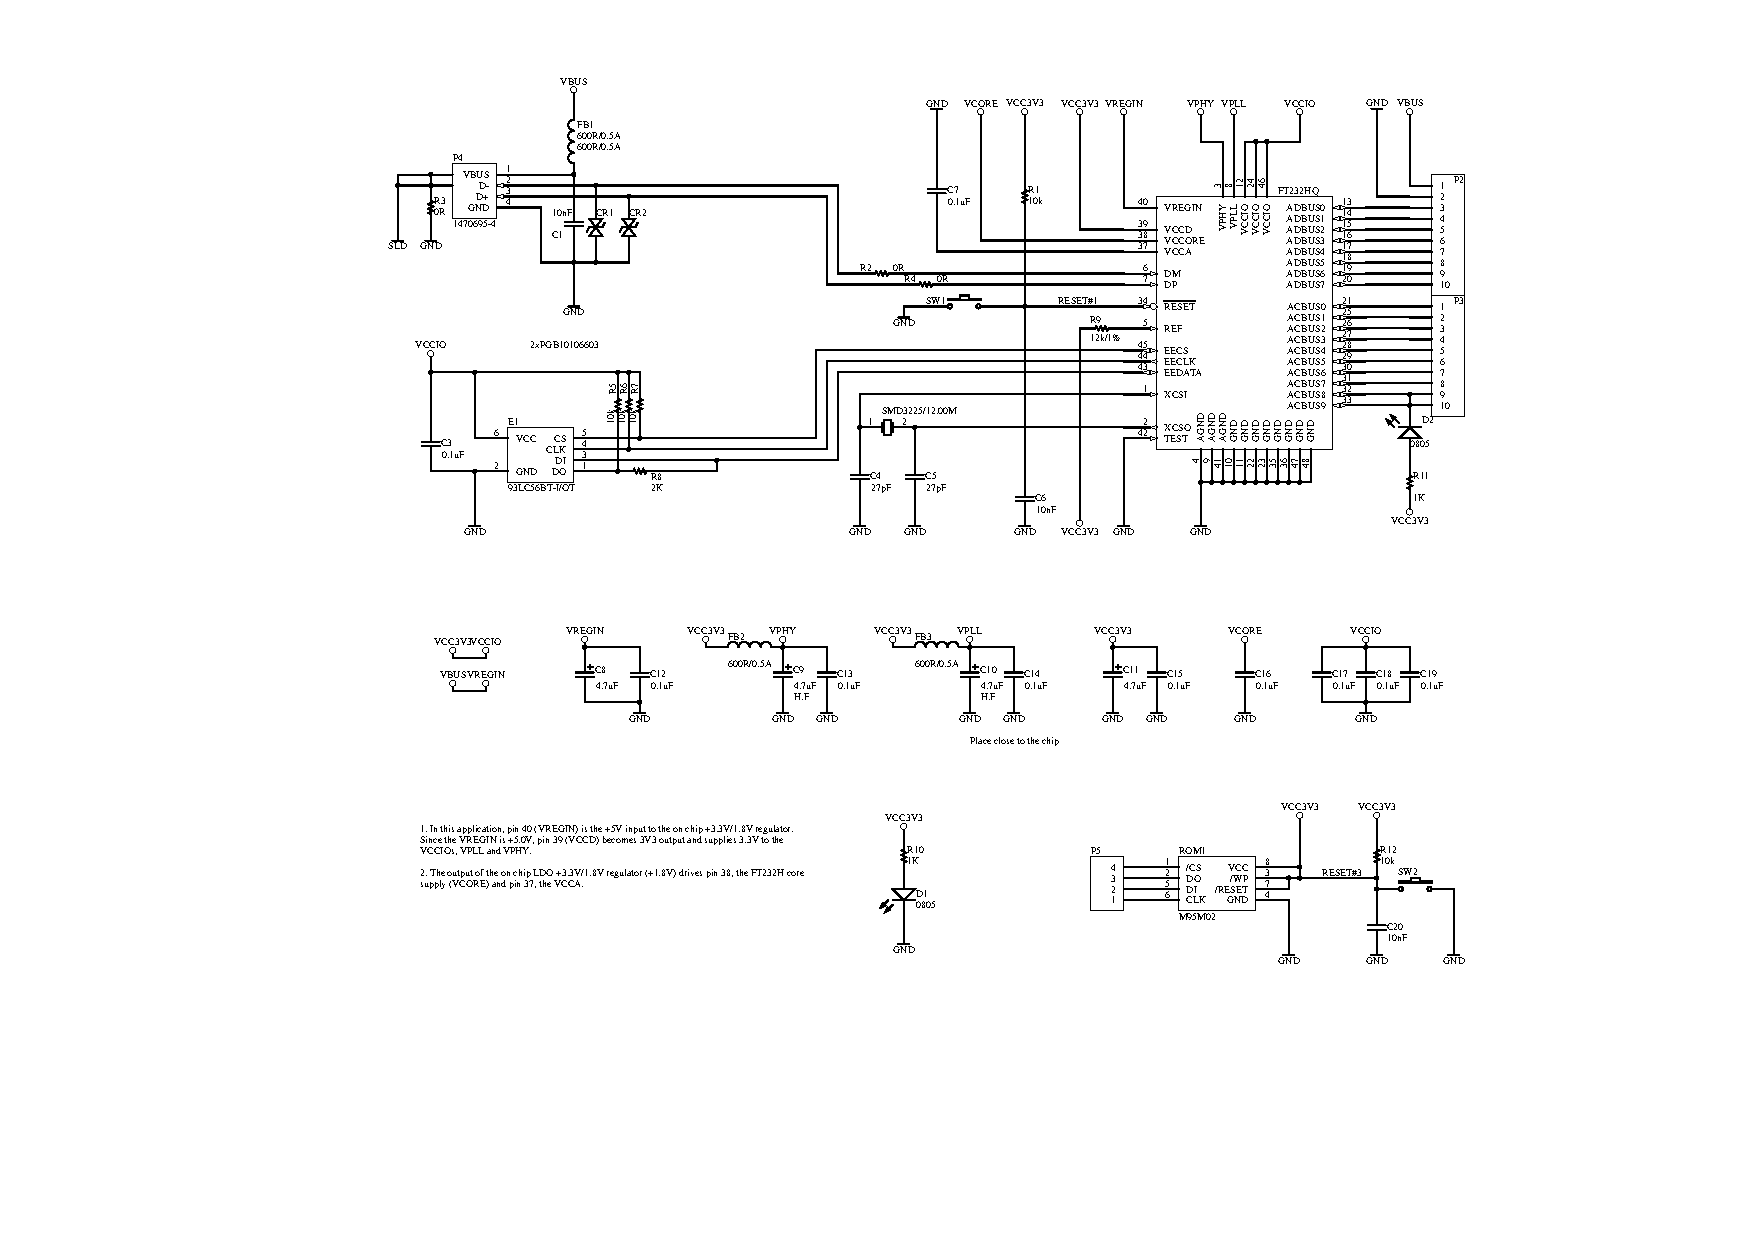
\includegraphics[width=\textwidth]{figures/Sheet1.pdf}
	\caption{OBD 系统电路原理图}\label{fig:sheet}
\end{figure}
 

\chapter{OBD 系统 PCB 电路图}

\begin{figure}[h]
	\centering
	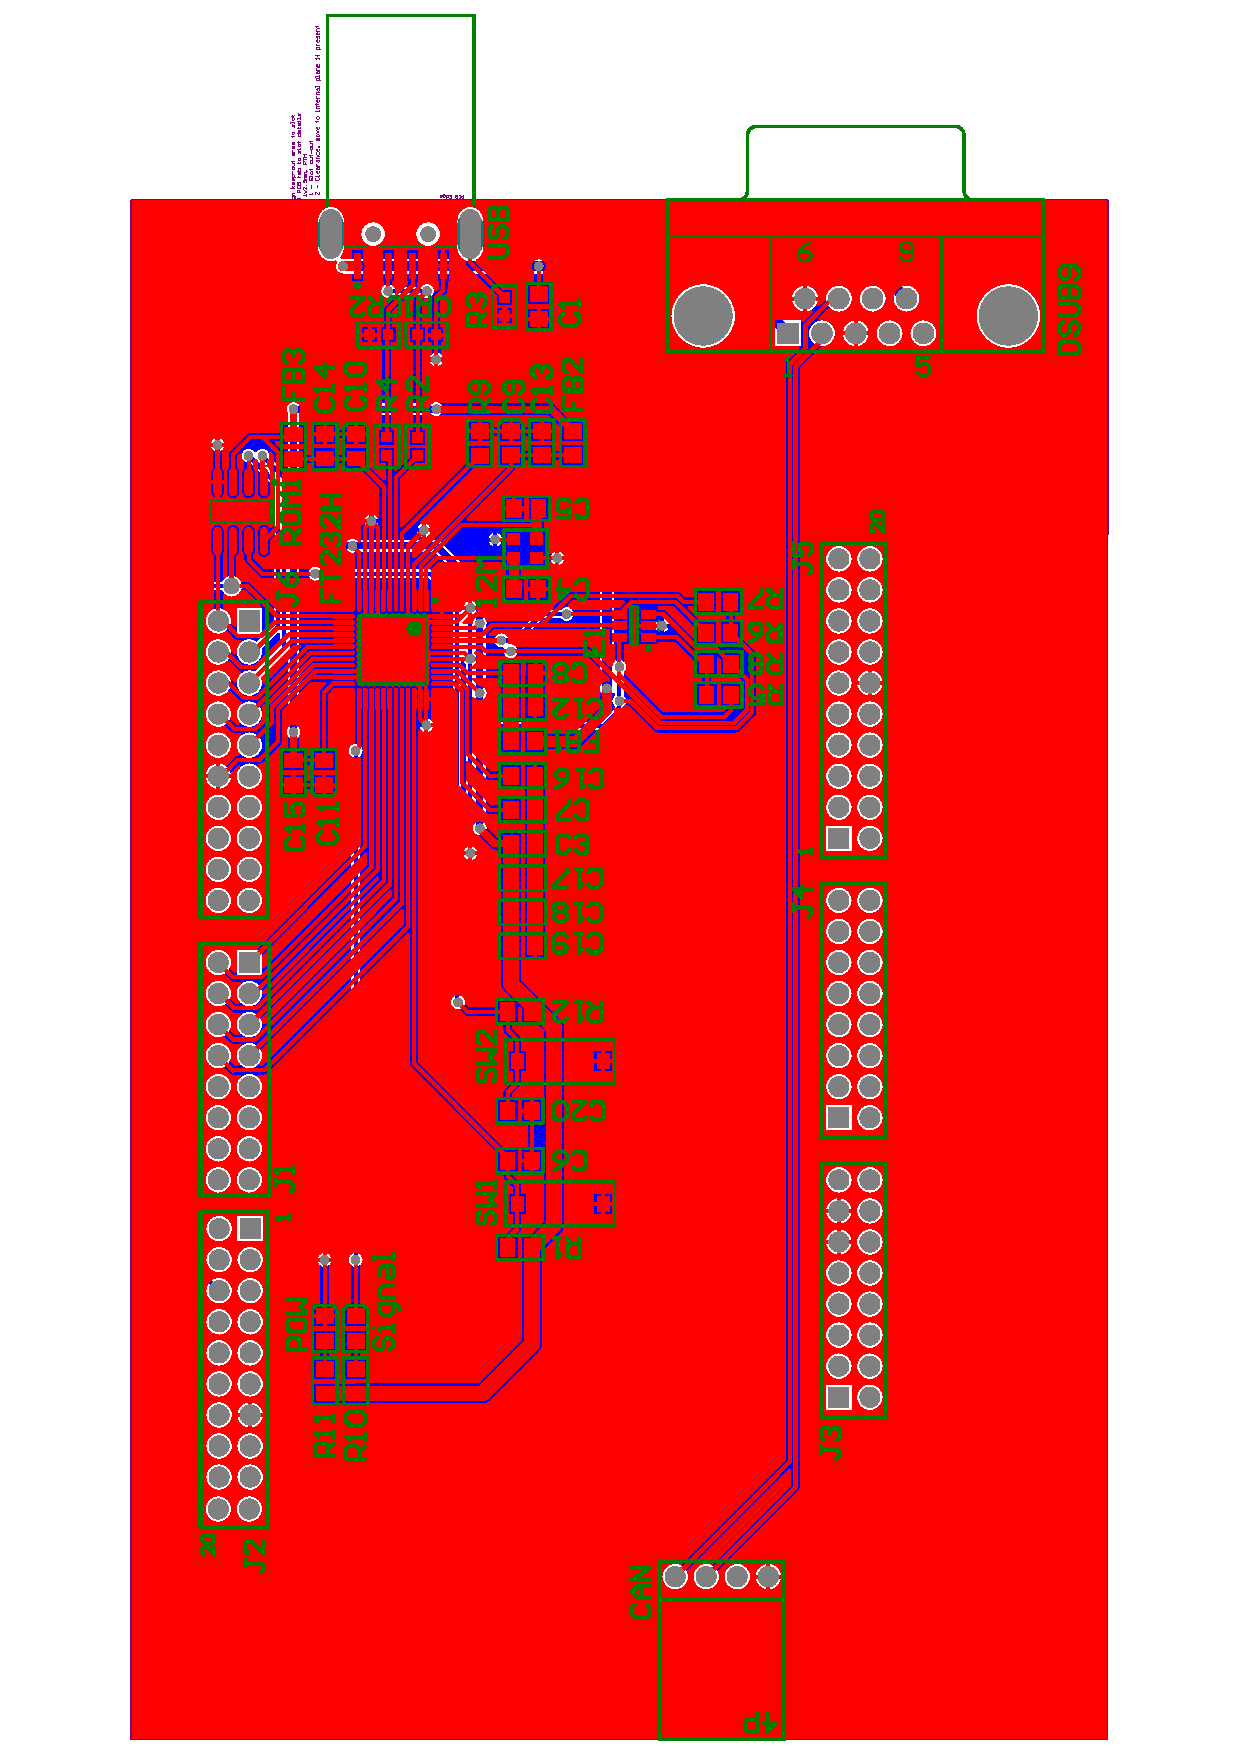
\includegraphics[width=0.7\textwidth]{figures/PCB1.pdf}
	\caption{OBD 系统 PCB 电路图}\label{fig:PCB}
\end{figure}
 

\backmatter
% 作者简介(博士论文需要)
%%%==================================================
%% resume.tex for BIT Master Thesis
%% modified by yang yating
%% version: 0.1
%% last update: Dec 25th, 2016
%%==================================================

\begin{resume}

本人…。

\end{resume}



\end{document}
